\documentclass[a4paper, 11pt]{article}

\usepackage[absolute]{textpos} % absolute positioned text blocks
\setlength{\TPHorizModule}{1mm}
\setlength{\TPVertModule}{1mm}
\usepackage[english]{babel}
\usepackage{csquotes}

% Images
\usepackage{graphicx} % used for images
\graphicspath{ {./../img/} }
\usepackage[labelfont=bf]{caption}

% Formatting
\usepackage{geometry} % better margins for document
\usepackage{titlesec} % better control over title spacing 
\usepackage{tabularx} % better tables
\usepackage[hidelinks]{hyperref} % hrefs
\usepackage{totcount}
\usepackage{pgfplots}
\pgfplotsset{compat=1.16}
\pgfplotsset{
    colormap={cool}{rgb255(0cm)=(237,66,76); rgb255(0.5cm)=(255,255,255); rgb255(1cm)=(57,146,239)}
}
\usepgfplotslibrary{colorbrewer}

\usepackage{float} % image placement
\usepackage{amssymb} % math symbols

% Code listings
\usepackage{listings}
\usepackage{commath}
\usepackage{pifont}
\usepackage{xcolor}
\definecolor{codered}{rgb}{0.93,0.26,0.298}
\definecolor{codegrey}{rgb}{0.7,0.7,0.7}
\definecolor{codepink}{rgb}{0.737,0.47,0.823}
\definecolor{codeblue}{rgb}{0.227,0.572,0.937}
\definecolor{codegreen}{rgb}{0.441,0.664,0.286}
\definecolor{codestring}{rgb}{0.58,0,0.82}
\definecolor{backcolor}{rgb}{0.95,0.95,0.95}
\definecolor{lightgrey}{rgb}{0.8,0.8,0.8}

\lstdefinelanguage{HLSL}{
	morekeywords=[1]{
        % variables
        position,sphere,direction,stepSize,dirMultiplier,dScene,dOrigin,p,dMin,dMax,result,k,d1,d2,d3,i,ao,co,d,seed,cell,pCell,
        i,j,x,y,z,frequency,amplitude,current,total,maxValue,
        vpos,ppos,vd,pd,density,projectedSunDistance,sunColor,sunTransmittance,cloudDensity,worldPosition,
        lightTransmittance,sunDirection,lightStepSize,insideBoxDist,
	},
	morekeywords=[2]{
        % methods and functions
		distance,normalize,min,max,dot,pow,sin,cos,tan,fract,length,smoothstep,
        sphereHit,raymarch,sphereDistance,sceneSDF,estimateNormal,hardshadow,softshadow,blend,sphereSDF,boxSDF,
        difference,union,intersection,ambientOcclusion,voronoi,
        random2d,random,random3d,randomSeed,floor,fbm,
        noise,lightmarch,
        sampleDensity,getColorVoronoi,getColorPerlin,worldToScreenPos
	},
	morekeywords=[3]{
        % CONSTANTS
        STEP_SIZE,MAX_STEPS,MINIMUM_STEP_SIZE,SURFACE_DISTANCE,MAX_DISTANCE,EPSILON,
        AO_ITERATIONS,AO_INTENSITY,AO_STEP_SIZE,
        LACUNARITY,GAIN,OCTAVES,
    },
	% morekeywords=[4]{
    %     % Unity Variables
    %     _VoronoiScale,_VoronoiOffset,,_VoronoiOctaves,_VoronoiPersistance,_VoronoiDensityThreshold,_VoronoiDensityMultiplier,
    %     _PerlinScale,_PerlinOffset,_PerlinOctaves,_PerlinPersistance,_PerlinDensityThreshold,_PerlinDensityMultiplier,
    % },
    keywordstyle=[1]\color{codeblue},
    keywordstyle=[2]\color{codered},
    keywordstyle=[3]\color{codepink},
    % keywordstyle=[4]\color{codegreen},
	commentstyle=\color{codegrey},
	morestring=[b]", % defines that strings are enclosed in double quotes
	morestring=[b]', % defines that strings are enclosed in single quotes
    backgroundcolor=\color{backcolor},
    stringstyle=\color{codered},
    numberstyle=\tiny,
    basicstyle=\ttfamily\footnotesize,
    breakatwhitespace=false,
    breaklines=true,
    captionpos=b,
    keepspaces=true,
    numbers=left,
    numbersep=5pt,
    showspaces=false,
    showstringspaces=false,
    showtabs=false,
	tabsize=2,
    sensitive=false, % keywords are not case-sensitive
    morecomment=[l]{//}, % l is for line comment
    morecomment=[s]{/*}{*/}, % s is for start and end delimiter
    belowskip=2.5em,
    aboveskip=1em,
}

% Gantt charts
\usepackage{pgfgantt}

% drawings
\usepackage{tikz}
\usepackage{fontawesome}
\usetikzlibrary{positioning, shapes}
\usetikzlibrary{arrows.meta}
\geometry{
	a4paper,
	left=28mm,
	right=28mm,
    top=30mm,
    bottom=30mm
}

% Colors 
\RequirePackage{color}
\definecolor{bfhgrey}{rgb}{0.41,0.49,0.57}
\definecolor{brinkpink}{rgb}{1.0, 0.65, 0.79}
\definecolor{columbiablue}{rgb}{0.61, 0.87, 1.0}

% Glossary
\usepackage[toc]{glossaries}
\newacronym{hlsl}{HLSL}{ High Level Shading Language }
\newacronym{gpu}{GPU}{ Graphics Processing Unit }
\newglossaryentry{latex}{name=LaTeX, description={ A high-quality document preparation system designed for the production of technical and scientific documentation }}
\newglossaryentry{noisegeneration}{name=Noise generation, text={noise generation}, description={ Noise generation is used to generate textures of one or more dimension with seemingly random smooth transitions from black to white (zero to one) }}
\newglossaryentry{volumetricrendering}{name=Volumetric rendering, text={volumetric rendering}, description={ This describes a technique which takes a 3D volume of data and projects it to 2D. It is mostly used for transparent effects stored as a 3D image }}
\newglossaryentry{raymarching}{name=Ray marching, text={ray marching}, description={ Ray marching is a type of method to approximate the surface distance of a volumetric object, where a ray is cast into the volume and stepped forward until the surface is reached }}
\newglossaryentry{lightmarching}{name=Lightmarching, text={lightmarching}, description={ The same concept as \gls{raymarching}, but instead of being cast into the volume, it is cast towards the primary light source with a constant step }}
\newglossaryentry{convection}{name=Convection, text={convection}, description={ Convection describes the transfer of heat from movement of liquid or gas }}
\newglossaryentry{billboard}{name=Billboard, text={billboard}, description={ A 2D image always facing towards the main camera }}
\newglossaryentry{worldspace}{name=World space, text={world space}, description={ Coordinates defined with respect to a global Cartesian coordinate system }}
\newglossaryentry{polymesh}{name=Polymesh, text={polymesh}, description={ A polymesh is a 3D model composed of polygons or triangles }}
\newglossaryentry{lowpoly}{name=Low poly, text={low poly}, description={ A 3D polymesh with a relatively low count of polygons }}
\newglossaryentry{voxel}{name=Voxel, text={voxel}, description= { Short for \textit{volume element}, a voxel is a value (either a number or a vector) on a scalar or vector field }}
\newglossaryentry{scalarfield}{name=Scalar field, text={scalar field}, description={ A scalar field describes a typically three-dimensional grid of elements called \textit{voxels}, each containing a scalar value }}
\newglossaryentry{vectorfield}{name=Vector field, text={vector field}, description={ It is the same as a scalar field, except the voxels are vector values }}
\newglossaryentry{spheretracing}{name=Sphere tracing, text={sphere tracing}, description={ Sphere tracing describes an optimized algorithm of ray marching by using signed distance functions to approximate the surface distance of the volume }}
\newglossaryentry{sdf}{name=Signed distance function, text={signed distance function}, description={ A signed distance function, short SDF, returns a positive distance if the origin is outside the volume and a negative distance if it is inside the volume }}
\newglossaryentry{surfacenormal}{name=Surface normal, text={surface normal}, description={ A \textit{surface normal} or \textit{normal} is a vector which is perpendicular to a given geometry, like a triangle or polygon }}
\newglossaryentry{gradient}{name=Gradient, text={gradient}, description={ The \textit{gradient} denotes the direction of the greatest change of a scalar function }}
\newglossaryentry{penumbra}{name=Penumbra, text={penumbra}, description={ The partially shaded outer region of diffuse shadows. Also described as soft edges }}
\newglossaryentry{shapeblending}{name=Shape blending, text={shape blending}, description={ In SDFs, shapes can be seemingly blended together by returning a interpolated value of those distances }}
\newglossaryentry{ambientocclusion}{name=Ambient occlusion, text={ambient occlusion}, description={ Also known as contact shadows, this method darkens points in the scene that are not or only slightly exposed to the light and its environment }}
\newglossaryentry{noise}{name=Noise, text={noise}, description={ A randomly generated pattern, referring to \gls{procedural} pattern generation }}
\newglossaryentry{translucent}{name=Translucent, text={translucent}, description={ An object or substance that is translucent allows light to be passed through it, meaning it is rendered transparently to some degree }} 
\newglossaryentry{parameters}{name=Parameters, text={parameters}, description={ Shader variables exposed to the Unity Editor }} 
\newglossaryentry{sss}{name=Subsurface scattering, text={subsurface scattering}, description={ SSS is a mechanism of light transport in which light enters a translucent object, is scattered around and exits the material at a different point, resulting in illuminated areas where the material is thin }} 
\newglossaryentry{sunlightforwarding}{name=Sunlight forward scattering, text={sunlight forward scattering}, description={ The process of sunlight shining through and illuminating the clouds which cover the sun }} 
\newglossaryentry{sunlighttransmittance}{name=Sunlight transmittance, text={sunlight transmittance}, description={ In this matter, the same as \gls{sunlightforwarding} }} 
\newglossaryentry{cnn}{name=Convolutional neural network, text={convolutional neural network}, description={ A neural network that is able to classify images }} 
\newglossaryentry{gan}{name=Generative adverserial network, text={generative adverserial network}, description={ A set of two neural networks, where one generates images and the other tries to tell wether those images are real or generated }} 
\newglossaryentry{aabb}{name=Axis-aligned bounding box, text={axis-aligned bounding box}, description={ A non-rotated bounding box enclosing an object completely }} 
\newglossaryentry{computeshader}{name=Compute shader, text={compute shader}, description={ A shader which runs on the GPU but outside of the default render pipeline }} 
\newglossaryentry{fbm}{name=Fractal Brownian motion, text={fractal Brownian motion}, description={ Different iterations of continuously more detailed noise layered on top of each other }} 
\newglossaryentry{fractalnoise}{name=Fractal noise, text={fractal noise}, description={ In this matter, the same as \gls{fbm} }} 
\newglossaryentry{procedural}{name=Procedural, text={procedural}, description={ Created solely with algorithms and independant of any prerequisites }}
\newglossaryentry{histogram}{name=Histogram, text={histogram}, description={ A graphical representation of data like brightness or color distribution of a given photograph }}
\newglossaryentry{csg}{name=Constructive solid geometry, text={constructive solid geometry}, description={ Short CSG, stands for combining primitive geometric objects with Boolean operators }}
\makenoidxglossaries

\glsunset{gpu}

% Bibliography
\usepackage[backend=biber, style=ieee]{biblatex}
\addbibresource{partials/specification.bib}

% add another lavel of headings
%\setcounter{tocdepth}{4}
\setcounter{secnumdepth}{4}
\titleformat{\paragraph}
{\normalfont\normalsize\bfseries}{\theparagraph}{1em}{}
\titlespacing*{\paragraph}
{0pt}{3.25ex plus 1ex minus .2ex}{1.5ex plus .2ex}

\begin{document}

\color{black}

\title{\doctitle}
\author{\docauthor}
\date{\versiondate}

\newcounter{requirements}
\newtotcounter{versionnumber}
\newcommand{\docsubtitle}{Project documentation}
\newcommand{\docauthor}{Matthias Thomann}
\newcommand{\doctitle}{Procedural cloud shader}
\newcommand{\fieldofstudies}{BSc in Computer Science}
\newcommand{\specialisation}{Computer perception and virtual reality}
\newcommand{\prof}{Prof. Urs K\"unzler}

\newcommand{\versiondate}{\today}
\newcommand{\sectionref}[1]{\autoref{#1}}
\newcommand{\emptyline}{\vspace{\baselineskip}\\\noindent}

\titlespacing*{\section} {0pt}{7.5ex plus 1ex minus .2ex}{2.3ex plus .2ex}
\titlespacing*{\subsection} {0pt}{4.25ex plus 1ex minus .2ex}{1.5ex plus .2ex}

\pagenumbering{roman}
\setcounter{page}{3}

%% include BFH logo and HuCE-ml logo

\begin{titlepage}

\setlength{\unitlength}{1mm}

\begin{textblock}{20}[0,0](22,12)
    
\includegraphics[scale=1.0]{../img/BFH_Logo_B.png}
\end{textblock}

\begin{flushleft}

\vspace*{21mm}

\fontsize{26pt}{40pt}\selectfont
\textbf{\doctitle}	\\
\vspace{2mm}

\fontsize{16pt}{24pt}\selectfont\vspace{0.3em}
\docsubtitle
\vspace{5mm}

\fontsize{10pt}{12pt}\selectfont
\textbf{Project 2} \\

\fontsize{10pt}{12pt}\selectfont
The goal of this project is to research and implement a procedural, volumetric cloud shader. The following document reveals the process of creating such a shader from both a technical and mathematical perspective, considering different algorithms for techniques like noise generation and raymarching.
\begin{textblock}{150}(28,225)
\fontsize{10pt}{17pt}
\begin{tabbing}
xxxxxxxxxxxxxxxxxxxxx\=xxxxxxxxxxxxxxxxxxxxxxxxxxxxxxxxxxxxxxxxxxxxxxx \kill
Field of Studies:	\> \fieldofstudies	\\
Specialization:	    \> \specialisation	\\
Author:		        \> \docauthor \\
Supervisor:         \> \prof \\
Date:			    \> \versiondate \\
\end{tabbing}

\end{textblock}

\begin{textblock}{150}(28,280)
\noindent 
\color{bfhgrey}\fontsize{9pt}{10pt}\selectfont
Berner Fachhochschule | Haute \'ecole sp\'ecialis\'ee bernoise | Bern University of Applied Sciences
\color{black}\selectfont
\end{textblock}

\end{flushleft}

\end{titlepage}

\clearpage

\clearpage

\section*{Abstract}
Clouds contribute a great deal to the overall ambience in games and can be the cherry on top by filling the sky with life.
To get as close as possible to real clouds, this project engages in researching and prototyping a \gls{procedural}, volumetric cloud shader.
\emptyline
In order to achieve \gls{volumetricrendering}, the document dives into the concept of \gls{raymarching}, a group of methods used to render a 3D data set inside a container box to make it appear volumetric.
Several variants of it are expanded on, like constant step, traditional, and sphere-traced \gls{raymarching}. Additionally, to account for perception of depth, the volume can be shaded with the aid of \gls{surfacenormal} estimation.
\\
In the second part, 2D and 3D \gls{noise} generation algorithms like Perlin's and the Voronoi algorithm are explained in detail. With \gls{fbm}, the different layers of noise are then merged into one highly detailed noise texture.
\emptyline
At last, the goal of the project was to create prototypes in Unity Editor displaying both volumetric rendering and noise algorithms, of which all were created successfully.
Armed with the combined knowledge of the research results and prototypes, a final shader was created, able to render a completely \gls{procedural} and volumetric cloudscape.
\\
For future work, the shader could be expanded into a fully-fledged weather system with meteorologically accurate formation of clouds, rain, snow and much more.
\clearpage

\tableofcontents
\clearpage

\pagenumbering{arabic}

\nocite{online:realtime-volumetric-cloudscapes}
\nocite{online:volumetric-cloudscapes}
\nocite{online:raymarching-sdf}
\nocite{online:volumetric-rendering}
\nocite{online:thebookofshaders}
\nocite{online:sebastianlague}

\section{General}

\subsection{Purpose}
During this project, all gathered information and knowledge about the researched algorithms and techniques are written down in this document.

\subsection{Revision History}
\begin{tabularx}{\textwidth}{|c|c|c|X|}
    \hline
    \textbf{Version}         & \textbf{Date}     & \textbf{Name}     & \textbf{Comment}                  \\ \hline \addtocounter{versionnumber}{1}
    0.\arabic{versionnumber} & March 21, 2020    & Matthias Thomann  & Initial draft                     \\ \hline \addtocounter{versionnumber}{1}
    0.\arabic{versionnumber} & March 29, 2020    & Matthias Thomann  & Added first research results      \\ \hline
\end{tabularx}
\clearpage

\section{Natural Clouds}

\subsection{Formation}
Clouds, as seen in nature, consist of a visible body of tiny water droplets and frozen crystals. 
In their natural occurrence, clouds are mostly generated from a nearby source of moisture, usually in the form of water vapor. 
This composition of particles creates the pleasant look of a white-grayish "fluffy" mass, floating in the sky.
\\
Due to certain factors like altitude or water source, different types of cloudscapes can be formed. They vary in shape, \gls{convection}, density and more.
That makes different cloud types highly unique in terms of appearance.
\\
For now, those factors are regarded as nature's randomness. However, an approximation of randomness will be covered in \sectionref{section:noise-generation}.


\subsection{Types of Clouds}
\label{section:cloud-types}
Cloudscapes are given a genus and classified in multiple groups, mainly differing in altitude, meaning the distance from the earth's surface to the cloud formation.
The following four cloud genera stand out due to their distinctiveness. A realistic simulation of a cloud system would consist of a combination of these types, which is why they are displayed here.
\begin{figure}[ht]
    \centering
        \begin{minipage}{0.47\linewidth}
            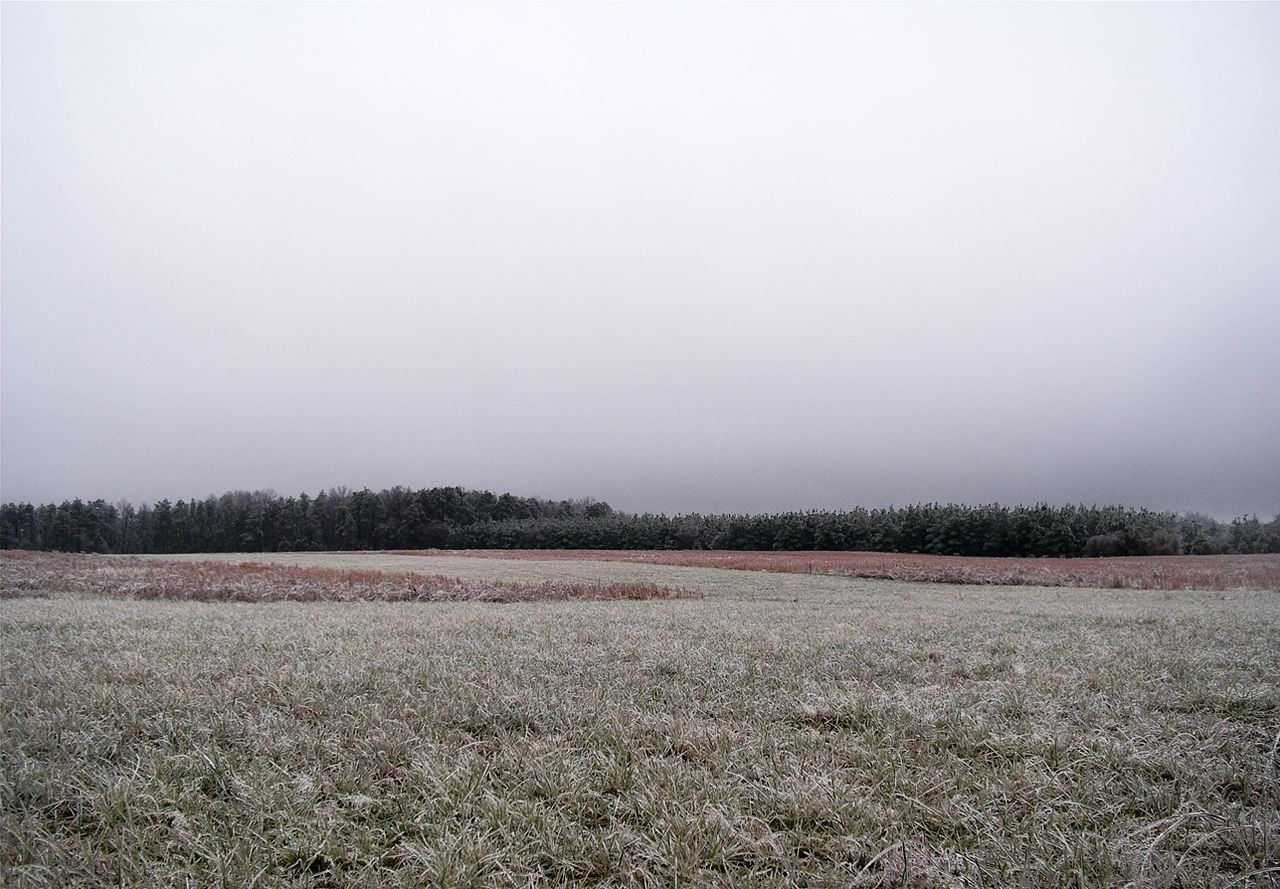
\includegraphics[width=\linewidth]{cloudforms-stratus}
            \captionof{figure}{Photographic reference of stratus clouds \protect\cite{img:cloudforms:stratus}.}
            \label{img:photo:cloudforms-stratus}        
        \end{minipage}        
    \hfill
        \begin{minipage}{0.47\linewidth}
            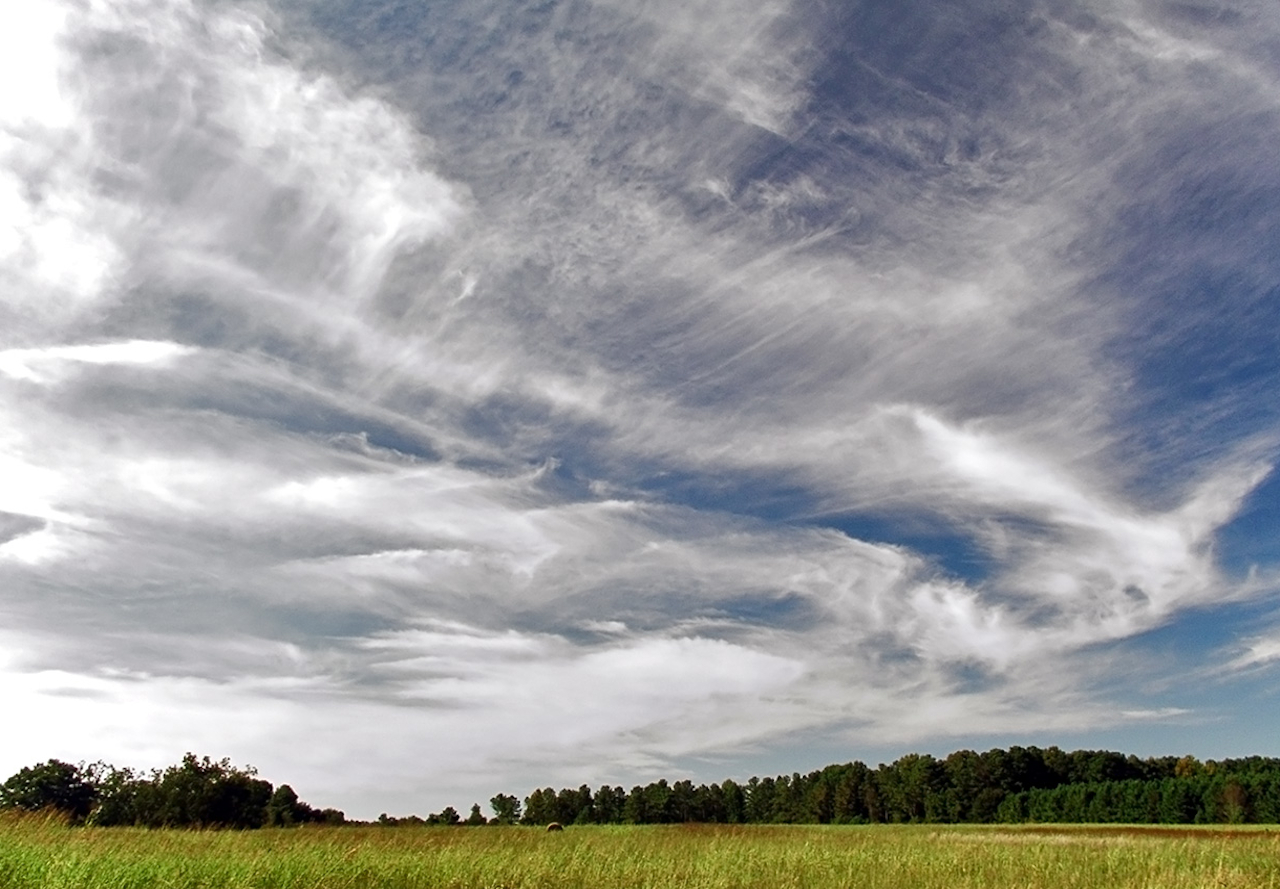
\includegraphics[width=\linewidth]{cloudforms-cirrus}
            \captionof{figure}{Photographic reference of cirrus clouds \protect\cite{img:cloudforms:cirrus}.}
            \label{img:photo:cloudforms-cirrus}        
        \end{minipage}
\end{figure}

\begin{figure}[ht]
    \centering
        \begin{minipage}{0.47\linewidth}
            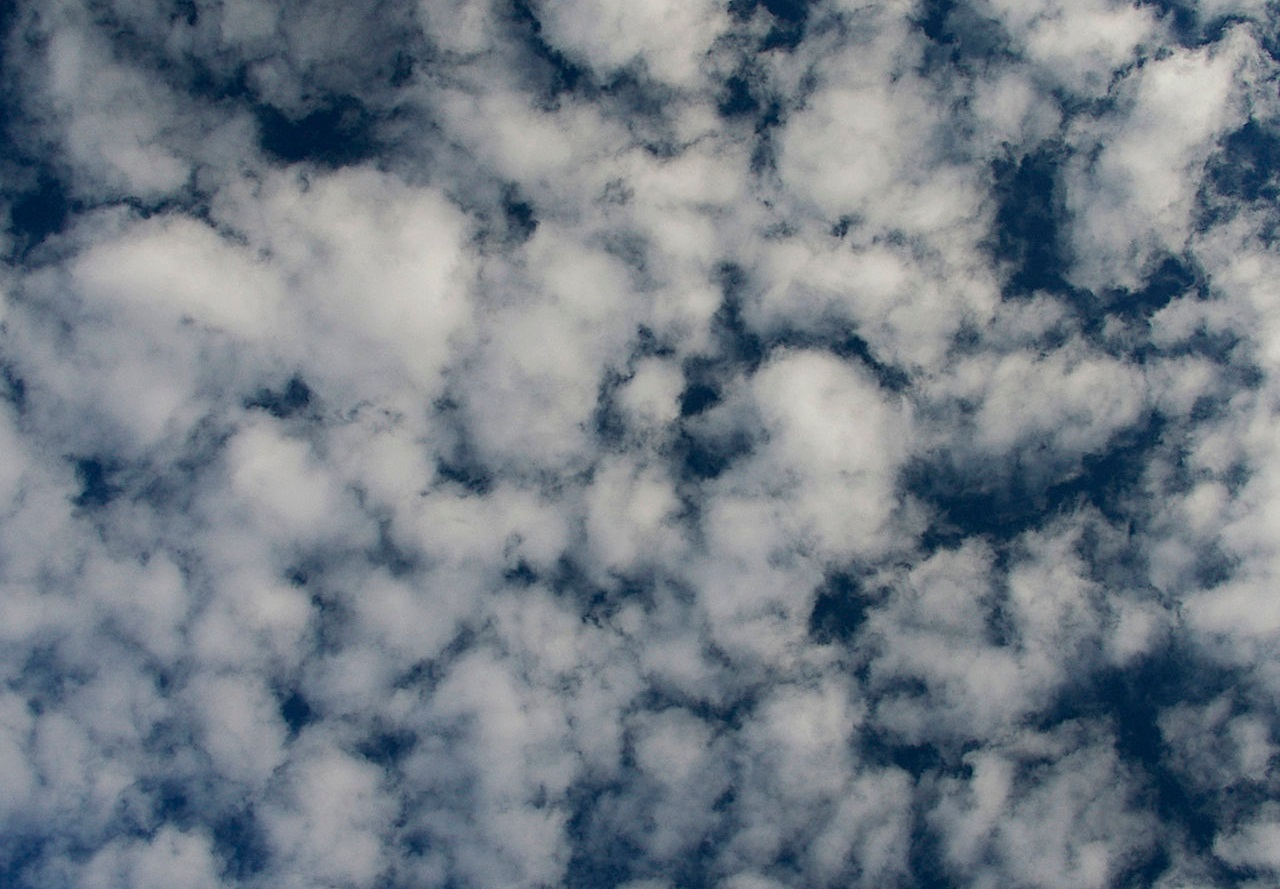
\includegraphics[width=\linewidth]{cloudforms-altocumulus}
            \captionof{figure}{Photographic reference of an altocumulus cloud formation \protect\cite{img:cloudforms:altocumulus}.}
            \label{img:photo:cloudforms-altocumulus}        
        \end{minipage}        
    \hfill
        \begin{minipage}{0.47\linewidth}
            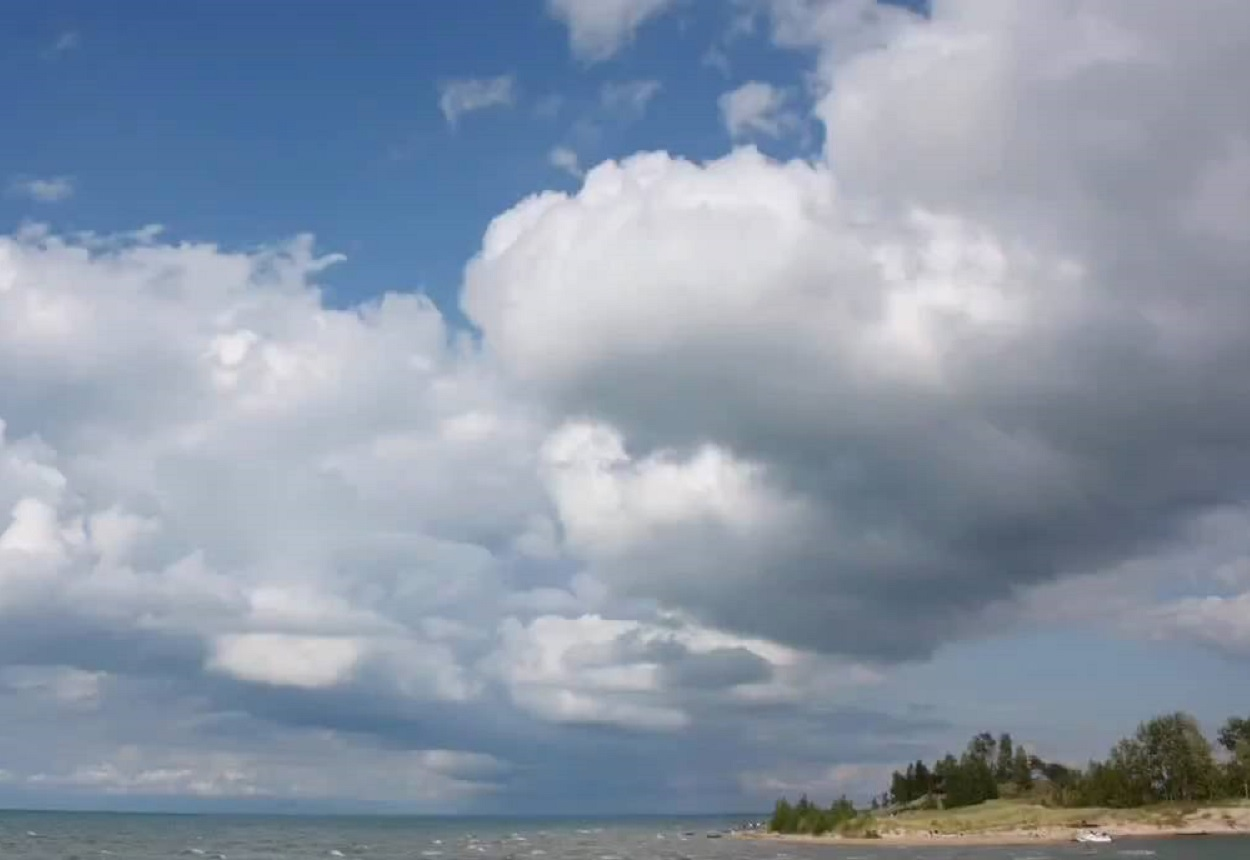
\includegraphics[width=\linewidth]{cloudforms-stratocumulus}
            \captionof{figure}{Photographic reference of stratocumulus cloudscape \protect\cite{img:cloudforms:stratocumulus}.}
            \label{img:photo:cloudforms-stratocumulus}        
        \end{minipage}
\end{figure}
\clearpage

\section{Clouds in Games}
\label{section:clouds-in-games}
Depicted in \autoref{img:photo:cloudforms-altocumulus} and \autoref{img:photo:cloudforms-stratocumulus} of \sectionref{section:cloud-types} are clouds of the genus \textit{cumulus}, which translated to English means \textit{heap} or \textit{pile}.
Their remarkable cotton-like look makes them easy to recognize, which is also why they are often used in games as a reference for "normal" clouds. 
That is also the reason why the prototypes are mainly related to this genus.
\\
In games, the formation as well as the natural composition are both irrelevant, as the clouds are essentially only used for cinematic ambience or as a mean to enhance the atmosphere. This leaves just the rendering technique and performance to worry about.

\subsection{Skyboxes}
A widespread solution for representing clouds in games is not rendering them at all, but instead using a set of polar sky dome images, also known as the skybox. This is a six-sided cube which is rendered around the whole game world. On each inward looking face of the cube, one of the sky dome images is displayed, creating a seamless sky around the inner side of the box.
\begin{figure}[H]
    \centering
        \begin{minipage}{0.47\linewidth}
            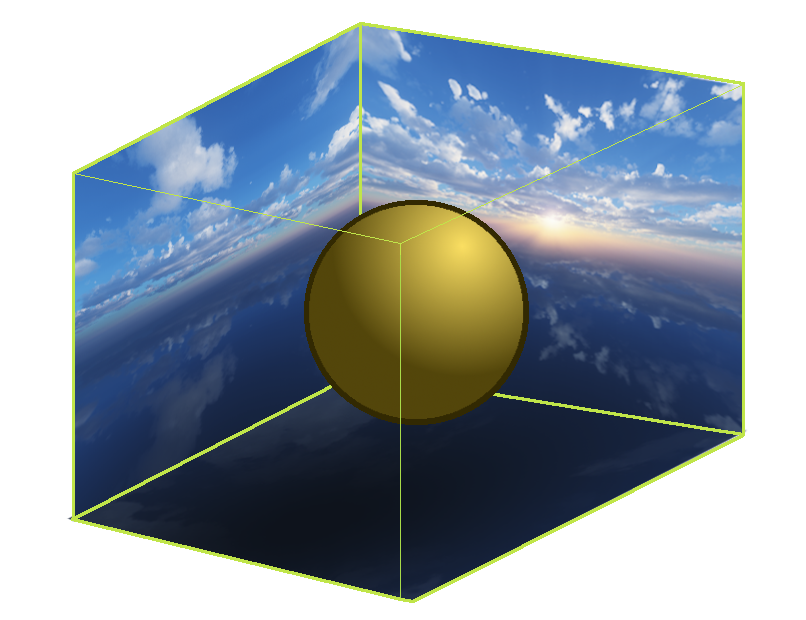
\includegraphics{edits/skybox}
            \captionof{figure}{The skybox cube as it is used in games.}
            \label{img:edits:skybox}
        \end{minipage}
    \hfill
        \begin{minipage}{0.45\linewidth}
            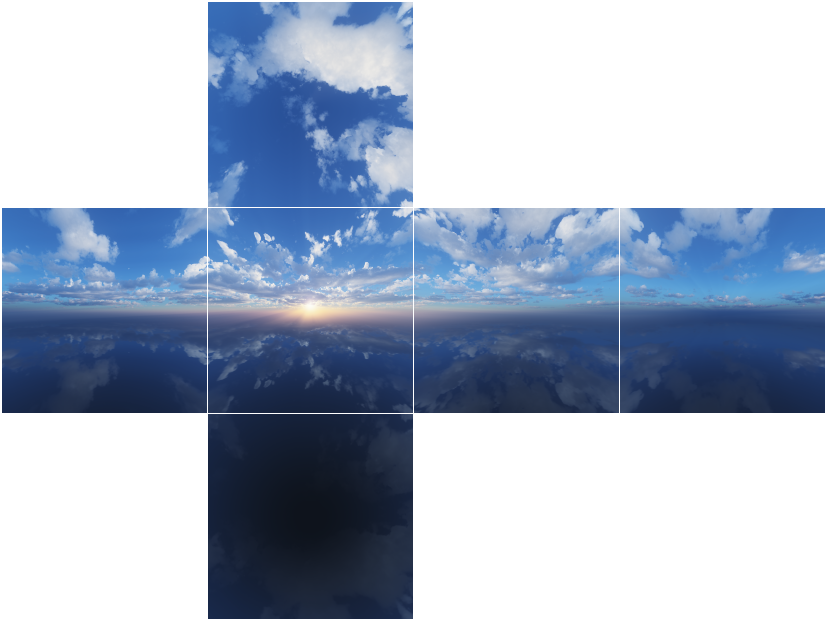
\includegraphics[width=\linewidth]{edits/skybox_layedout}
            \captionof{figure}{The polar sky dome images, folded out.}
            \label{img:edits:skybox_layedout}
        \end{minipage}
\end{figure}

\noindent
Besides rendering the sky, this of course allows clouds to be drawn right into the background. Also, in terms of performance, this is extremely cheap and efficient. On the other hand, it removes the ability for the clouds to move. 
They also have no volumetric body and no way of interaction with the game world.
\\
This method does indeed give the scenery a more cloudy look, but what is missing is the "feel", or in other words the motion, interaction and lifelikeness of the clouds.

\subsection{Billboards}
Similar to the approach with the skybox, this technique also only uses 2D images of clouds. They are rendered individually and are always facing the camera. This is called \textit{\gls{billboard}ing}.
Now that each cloud is represented by its own game object, having a position in \gls{worldspace} as well as a scale and many other properties, it is possible to animate the clouds. For example, by moving the game objects in a circle around the world, the clouds seemingly "pass by".
\begin{figure}[H]
    \centering
        \begin{minipage}{0.48\linewidth}
            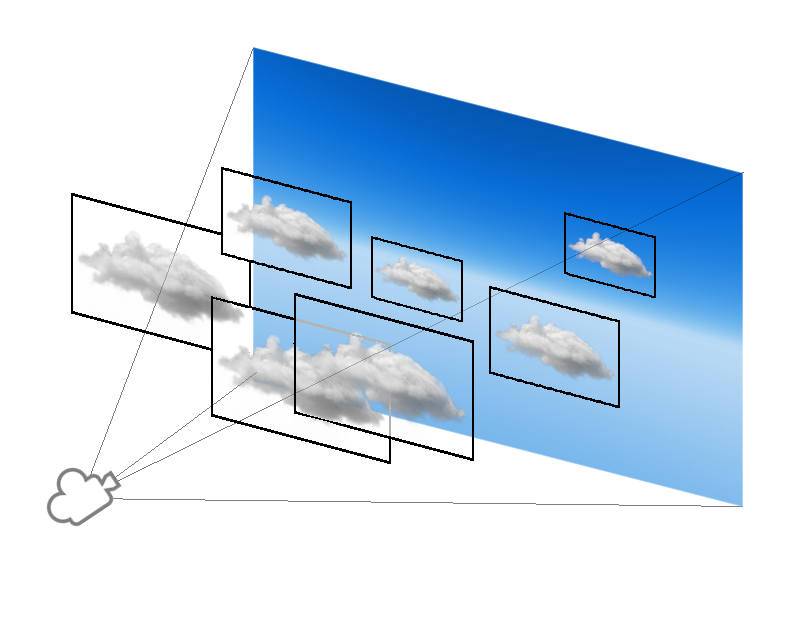
\includegraphics{edits/billboards}
            \captionof{figure}{A collection of 2D cloud billboards facing the camera.}
            \label{img:edits:billboards}
        \end{minipage}
    \hfill
        \begin{minipage}{0.45\linewidth}
            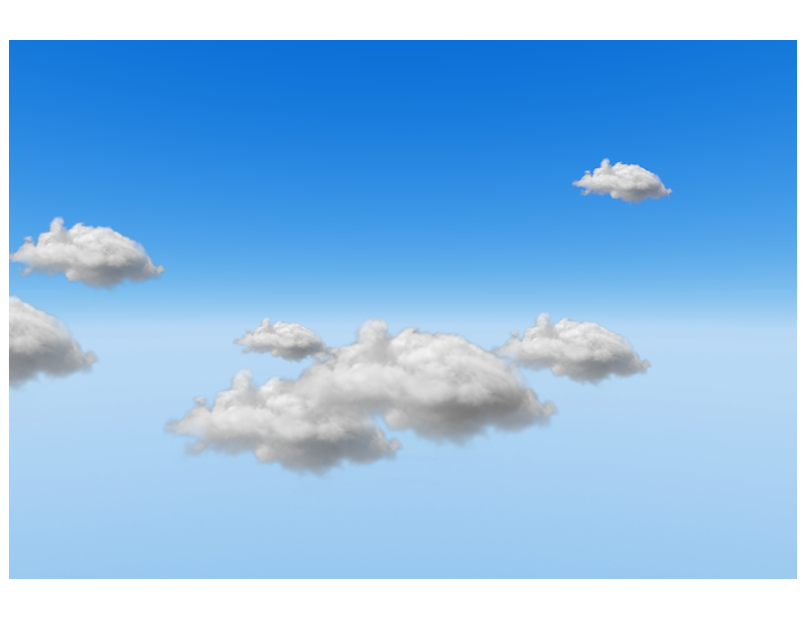
\includegraphics[width=\linewidth]{edits/billboards_rendered}
            \captionof{figure}{The rendered result of the image to the left.}
            \label{img:edits:billboards_rendered}
        \end{minipage}
\end{figure}
\noindent
Due to billboarding, the orientation is already given, making the overall rendering time and effort of this technique quite advantageous to others.
\\
The major flaw of using billboards is of course that they are still 2D images, meaning they cannot really change appearance and therefore, do not evolve at all. 
Still, for many games, this technique suffices in the required diversity of background scenery and does not exceed the allowed performance share for such a task.

\subsection{Mesh-based Objects}
It is imaginable to simply use a \gls{polymesh} shaped like a cloud and render that like any other game object. By adding a texture, this would make for some decent looking clouds.
\\
However, the level of detail of such a polymesh is directly connected to the amount of vertices and faces that have to be processed every frame.
As seen in \autoref{img:rendered:cloud-mesh}, there are hundreds of polygons required to merely represent the basic shape of a realistic cloud.
If a similarly complex mesh is to be used for every cloud, a massive overhead is generated for objects that usually only contribute to the background of a game.
\begin{figure}[H]
    \centering
    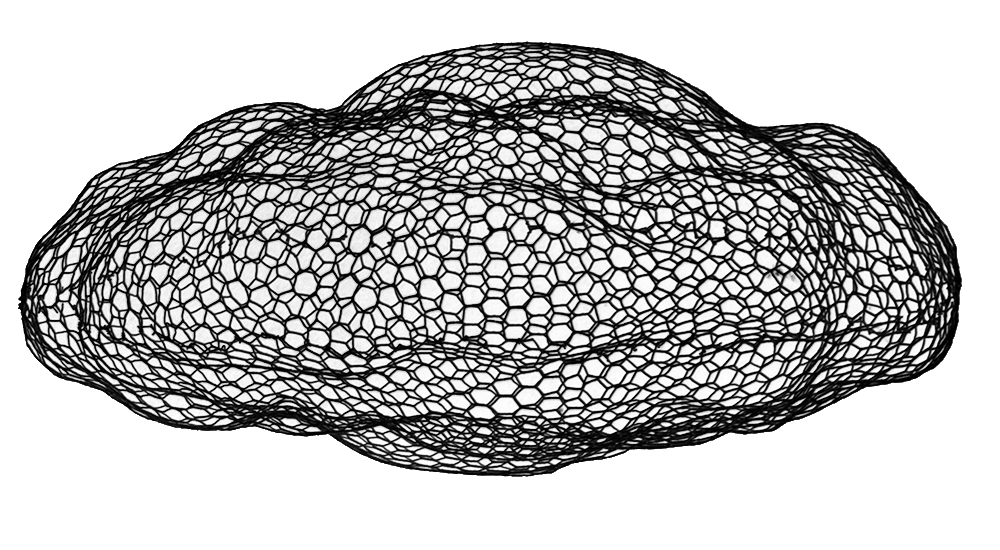
\includegraphics[width=0.5\linewidth]{rendered-cloud-mesh}
    \captionof{figure}{A \gls{polymesh} in the shape of an altocumulus cloud \cite{img:rendered:cloud-mesh}.}
    \label{img:rendered:cloud-mesh}
\end{figure}
\noindent
Apart from the performance impact, this method offers a volumetric, possibly interactable object just like any other 3D model does.
When massively decreasing the polygon count and therefore relinquishing the realistic look, mesh-based objects may be a viable solution for some \gls{lowpoly} games.
Otherwise, it is not reasonable to use this method.

\subsection{Volumetric Clouds}
Finally, clouds can be rendered via a technique called \textit{volumetric rendering}. The images below show volumetric cloudscapes as seen in popular video games of major publishers.
The method itself is explained in detail in \sectionref{section:volumetric-rendering}.

\begin{figure}[H]
    \centering
    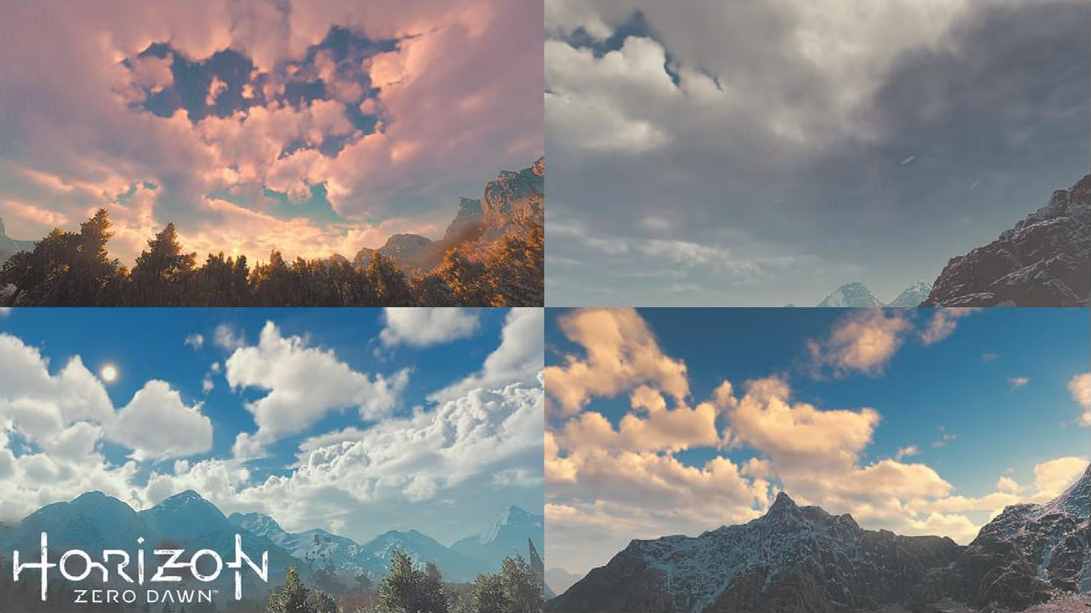
\includegraphics[width=\linewidth]{rendered-clouds-zerodawn}
    \captionof{figure}{Several volumetric cloudscapes from the game \textit{Horizon: Zero Dawn}, drawn in real time \protect\cite{img:rendered:clouds-zerodawn}.}
    \label{img:rendered:clouds-zerodawn}
\end{figure}
\clearpage

\section{Volumetric Rendering}
\label{section:volumetric-rendering}

\subsection{Definition}
\Gls{volumetricrendering} describes a technique for generating a visual representation of image data that is stored in a 3D volume. 
This especially comes to use for visual effects that are volumetric in nature, like fluids, clouds, fire, smoke, fog and dust, which are all extremely difficult or even impossible to model with geometric primitives.
\\
In addition to rendering such effects, volumetric rendering has become essential to scientific applications like medical imaging, for which a typical 3D data volume is a set of 2D slice images acquired by a CT (computed tomography) or MRI (magnetic resonance imaging) scanner.
\emptyline
The data volume is also called a \textit{\gls{scalarfield}} or \textit{\gls{vectorfield}}, which associates a scalar or vector value, called \textit{\gls{voxel}} (short for \textit{volume element}), to every point in the defined space.
For a scalar field, it can be imagined like a 3D grid, where each point holds a single number. This number could, for example, represent the density of a cloud at that very point. A vector field holds an n-tuple at each grid point.

\subsection{Preliminary Notes}
Most of the figures in the upcoming subsections depict only a single ray. However, this is only for explanatory purposes. The process has to be executed not once, but for each fragment processed by the fragment shader.

\subsection{Constant Step Ray Marching}
To actually render the volume data, a method called \textit{\gls{raymarching}} is used. With it, the surface distance of the volumetric data is approximated by creating a ray from the camera to the object for each fragment. The ray is then extended into the volume of the object and stepped forward until the surface is reached.

\begin{figure}[H]
    \centering
    \begin{tikzpicture}[scale=0.7]
        \node[cyan] at (3.0,3.25) {\textbullet};
        \node[cyan] at (3.5,3.50) {\textbullet};
        \node[cyan] at (4.0,3.73) {\textbullet};
        
        \draw (0,0) -- (5,0) -- (5,5) -- (0, 5) -- (0, 0);
        \draw (2,1) -- (7,1) -- (7,6) -- (2, 6) -- (2, 1);
        \draw (0,0) -- (2,1); \draw (5,0) -- (7,1); \draw (5,5) -- (7,6); \draw (0,5) -- (2,6); 

        \node[rotate=30,anchor=west] (cam) at (-1.5,1) {\faVideoCamera};
        \node[red] (frag) at (2.5,3) {\ding{53}};
        \node[red] at ($(frag) + (1,-0.5)$) {fragment};
        \draw[red,shorten >=-8pt] (cam) node[below right]{} -- (frag);
        \draw[-{Latex[length=2mm]},shorten <=-6pt,cyan] (frag) -- (4.75,4.125) node[above,xshift=0.1cm] {stepped forward};

    \end{tikzpicture}
    \captionof{figure}{Ray marching concept visualized.}
\end{figure}

\noindent
The ray-surface intersection is not directly calculated because it is not exactly defined for volumes like clouds, which is why the surface distance is approximated instead.

\pagebreak
\noindent
In \gls{raymarching}, the algorithm only knows when it has reached the surface, or to be precise, when it is inside the actual object volume.
\\
With this information, it is only possible to extend the ray in steps of a predefined length until the inside of the object is reached.
With a constant step, the approximation of the surface distance is exactly as precise as the size of the constant step.
\\
Once the ray is inside the actual volume, the functions returns the distance for this ray.

\begin{figure}[H]
    \centering
    \begin{tikzpicture}[scale=1.2]
        \tikzset{edge/.style = {-{Latex[length=3mm]}}}
        \tikzset{smalledge/.style = {-{Latex[length=1mm]}}}

        % ray
        \node[rotate=6] (cam) at (0,2) {\faVideoCamera};
        \draw[edge] (cam) node[above,xshift=1cm,rotate=6]{ray} -- (10,3);
        \node (1) at (2,2.2) {\textbullet};
        \node (2) at (3,2.3) {\textbullet};
        \node (3) at (4,2.4) {\textbullet};
        \node (4) at (5,2.5) {\textbullet};
        \node (5) at (6,2.6) {\textbullet};
        \node (6) at (7,2.7) {\textbullet};
        \node[cyan] (7) at (8,2.8) {\textbullet};

        % surf dist
        \draw[red] (2,1.5) -- (2.5,2) -- (4,1.8) -- (5,1.5) -- (7.4,2) -- (7.7,4) -- (9,4.3);
        \node[red,rotate=11] at (6.35, 1.6) {volume boundaries};

        % ray steps
        \draw[smalledge] (1) edge[bend left=60] node [left]{} (2);
        \draw[smalledge] (2) edge[bend left=60] node [left]{} (3);
        \draw[smalledge] (3) edge[bend left=60] node [left]{} (4);
        \draw[smalledge] (4) edge[bend left=60] node [left]{} (5);
        \draw[smalledge] (5) edge[bend left=60] node [left]{} (6);
        \draw[smalledge] (6) edge[bend left=60] node [left]{} (7);

        % returns text
        \draw[cyan, shorten <=-0.2cm] (7) -- (9,3.7) -- (11,3.7) node[xshift=-1cm,above]{function returns};

        \end{tikzpicture}
    \captionof{figure}{Traditional ray marching.}
\end{figure}

\noindent
An implementation of this algorithm can be seen in \autoref{lst:shader:raymarch:constantstep}. Note that the volume to be rendered in this example is just a simple sphere.
Also, the purple texts represent constants. Exact values for them are evaluated during prototyping.

\begin{lstlisting}[language=HLSL, numbers=left, caption=Implementation of a ray march function with constant step.,captionpos=b, label=lst:shader:raymarch:constantstep]
// position:  the sampling point along the ray.
// direction: the ray's direction.
fixed4 raymarch(float3 position, float3 direction)
{
    for (int i = 0; i < MAX_STEPS; i++)
    {
        if (sphereHit(position))
            return fixed4(1,0,0,1);
        
        position += normalize(direction) * STEP_SIZE;
    }
    
    return fixed4(0,0,0,1);
}
\end{lstlisting}

\noindent
In order to check if the ray is inside the volume, the function \lstinline[language=HLSL]{sphereHit()} is used.

\begin{lstlisting}[language=HLSL, numbers=left, caption=Implementation of a volume distance function for a sphere.,captionpos=b, label=lst:shader:raymarch:spherehit]
bool sphereHit(float3 position) {
    float4 sphere = float4(0, 1, 0, 1);
    return distance(sphere.xyz, position) < sphere.w;
}
\end{lstlisting}

\pagebreak
\subsection{Traditional Ray Marching}
It is obvious to see that the constant step \gls{raymarching} can only result in an accurate approximation of the surface distance if the step size is relatively small.
This has a direct impact on performance and thus, is not a viable solution for the problem.
\\
In traditional \gls{raymarching}, an optimization has been developed for this problem. The algorithm does not blindly step forward, but instead tries to get as close to the real distance as possible.
After the volume is reached, the step size is decreased and the ray steps out of the volume again. It then tries to approximate the surface distance by stepping in and out repeatedly in continuously smaller steps, thus converging towards the exact intersection.
Once the step size falls below a certain threshold, the distance approximation is assumed to be precise enough and the value is returned for that ray march.

\begin{figure}[H]
    \centering
    \begin{tikzpicture}[scale=1.2]
        \tikzset{edge/.style = {-{Latex[length=3mm]}}}
        \tikzset{smalledge/.style = {-{Latex[length=2mm]}}}

        % ray
        \node[rotate=6] (cam) at (0,2) {\faVideoCamera};
        \draw[edge] (cam) node[above,rotate=6,xshift=1cm]{ray} -- (10,3);
        \node (1) at (2,2.2) {\textbullet};
        \node (2) at (4,2.4) {\textbullet};
        \node (3) at (6,2.6) {\textbullet};
        \node[cyan] (4) at (8,2.8) {\textbullet};

        % surf dist
        \draw[red] (2,1.5) -- (2.5,2) -- (4,1.8) -- (5,1.5) -- (7.4,2) -- (7.7,4) -- (9,4.3);

        % reverse nodes
        \node[cyan] (5) at (7,2.7) {\textbullet};
        \node[cyan] (6) at (7.5,2.75) {\textbullet};

        % ray steps
        \draw[smalledge] (1) edge[bend left=60] node [left]{} (2);
        \draw[smalledge] (2) edge[bend left=60] node [left]{} (3);
        \draw[smalledge] (3) edge[bend left=60] node [left]{} (4);

        % ray reverse steps
        \draw[smalledge,cyan,shorten >=-0.1cm,shorten <=-0.1cm] (4) edge[bend left=60] node [left]{} (5);
        \draw[smalledge,cyan,shorten >=-0.1cm,shorten <=-0.1cm] (5) edge[bend left=60] node [left]{} (6);

        % close enough
        \draw[cyan, shorten <=-0.2cm] (6) -- (9,3.7) -- (11,3.7) node[xshift=-1cm,above]{step size small enough};
        
        \end{tikzpicture}
    \captionof{figure}{Traditional ray marching.}
\end{figure}

\noindent
As visible, the traditional \gls{raymarching} ends up with a more accurate result and the amount of steps per ray could be relatively lower, ultimately saving performance. 
\\
However, there is still an issue. The algorithm may jump in and out of the volume, even if it would already be precise enough, essentially taking unnecessary steps.

\begin{lstlisting}[language=HLSL, numbers=left, caption=Implementation of a traditional ray march function with converging surface distance approximation.,captionpos=b, label=lst:shader:raymarch:traditional]
fixed4 raymarch(float3 position, float3 direction)
{
    float stepSize = STEP_SIZE;
    float dirMultiplier = 1;
    for (int i = 0; i < MAX_STEPS; i++)
    {
        if (stepSize < MINIMUM_STEP_SIZE)
            return fixed4(1,0,0,1);

        if (sphereHit(position)) {
            // reduce step size by half and invert marching direction.
            stepSize /= 2;
            dirMultiplier = -1;
        } else {
            dirMultiplier = 1;
        }
        
        position += normalize(direction) * stepSize * dirMultiplier;
    }
    
    return fixed4(0,0,0,1);
}
\end{lstlisting}

\pagebreak
\subsection{Sphere Tracing}
An even better approach to approximate the intersection of the ray and the volume is called \textit{\gls{spheretracing}}. 
Instead of evaluating if the ray is inside the volume or not, an exact distance to the scene is measured. This distance is the minimum amount of space the algorithm can march along its ray without colliding with anything.
For that, a function group called \textit{\gls{sdf}s} is used.

\subsubsection{Signed Distance Functions}
A \gls{sdf} (SDF) returns the shortest distance from a given point in space to some surface.
The sign of the returned value indicates whether that point is inside the surface or outside, hence the name.
\\
For example, the \gls{sdf} $f(p)$ for a point $p=(p_1, p_2, p_3)$ to the surface of a sphere $s=(s_1, s_2, s_3)$ with radius $R$ looks like this:
$$ f(p) = \sqrt{(s_1 - p_1)^2 + (s_2 - p_2)^2 + (s_3 - p_3)^2} - R $$

\noindent
This translates into a simple code snippet, mostly identical to the function \lstinline[language=HLSL]{sphereHit()} in \autoref{lst:shader:raymarch:spherehit}, except the distance is returned instead of a Boolean.
\begin{lstlisting}[language=HLSL, caption=Implementation of a signed distance function for a sphere., label=lst:shader:raymarch:spheredistance]
float sceneSDF(float3 position) {
    float4 sphere = float4(0, 0, 0, 1);
    return distance(sphere.xyz, position) - sphere.w;
}
\end{lstlisting}

\noindent
With the sphere in the example being at the origin and having $R = 1$, a positive distance is returned for points outside the sphere and a negative distance if the point is inside the sphere.
\begin{lstlisting}[language=HLSL]
float d1 = sceneSDF(float3(2, 0, 0));   // d1 = 1.0
float d2 = sceneSDF(float3(0, 0.5, 0)); // d2 = -0.5
float d3 = sceneSDF(float3(5, -5, 5));  // d3 = 7.66
\end{lstlisting}

\subsubsection{Sphere Tracing with SDFs}
If the distance to the scene can be calculated with a \gls{sdf}, the algorithm becomes rather straight forward. The distance to the scene is evaluated at the start, then one can freely march along the ray for that amount of distance. Once arrived at the new point, the process is repeated until the SDF returns a small enough value.

\begin{figure}[H]
    \centering
    \begin{tikzpicture}[scale=1.2]
        \tikzset{edge/.style = {-{Latex[length=3mm]}}}

        % ray
        \node[rotate=6] (cam) at (0,2) {\faVideoCamera};
        \draw[edge] (cam) node[above,rotate=6,xshift=1cm]{ray} -- (10,3);
        \node (1) at (2,    2.2) {\textbullet};
        \node (2) at (2.5,  2.25) {\textbullet};
        \node (3) at (2.75, 2.275) {\textbullet};
        \node (4) at (3.05, 2.305) {\textbullet};
        \node (5) at (3.42, 2.342) {\textbullet};
        \node (6) at (3.88, 2.388) {\textbullet};
        \node (7) at (4.44, 2.444) {\textbullet};
        \node (8) at (5.18, 2.518) {\textbullet};
        \node (9) at (6.14, 2.614) {\textbullet};
        \node (10) at (6.99, 2.699) {\textbullet};

        \draw (1) circle  (0.5);
        \draw (2) circle  (0.25);
        \draw (3) circle  (0.3);
        \draw (4) circle  (0.37);
        \draw (5) circle  (0.46);
        \draw (6) circle  (0.56);
        \draw (7) circle  (0.74);
        \draw (8) circle  (0.96);
        \draw (9) circle  (0.85);
        \draw (10) circle (0.49);

        % surf dist
        \draw[red] (2,1.5) -- (2.5,2) -- (4,1.8) -- (5,1.5) -- (7.4,2) -- (7.9,4.1) -- (9,4.4);

        % distance small enough
        \node[cyan] (11) at (7.48, 2.748) {\textbullet};
        \draw (11) circle (0.1);
        \draw[cyan, shorten <=-0.2cm] (11) -- (9,3.7) -- (11,3.7) node[xshift=-1cm,above]{scene distance small enough};
        
        \end{tikzpicture}
    \captionof{figure}{Ray marching with SDF-based sphere tracing.}
    \label{img:tikz:rendering:spheretracing}
\end{figure}

\noindent
As seen in \autoref{img:tikz:rendering:spheretracing}, the result is highly accurate.
For the previous example with just one single sphere as a volume, the algorithm can be implemented like in \autoref{lst:shader:raymarch:spheretracing}.

\begin{lstlisting}[language=HLSL, caption=Implementation of ray marching with sphere tracing., label=lst:shader:raymarch:spheretracing]
float raymarch (float3 position, float3 direction)
{
    float dOrigin = 0.0;
    for (int i = 0; i < MAX_STEPS; i++)
    {
        float dScene = sceneSDF(position + dOrigin * direction);
        if (dScene < SURFACE_DISTANCE || dScene > MAX_DISTANCE)
            break;

        dOrigin += dScene;
    }
    return dOrigin;
}
\end{lstlisting}

\noindent
In order to save on performance, it is imperative to break the loop when \lstinline[language=HLSL]{distanceScene} exceeds \lstinline[language=HLSL]{MAX_DISTANCE}. This way, the distance evaluation for that ray can be stopped earlier than waiting for the loop to complete.
Another example why this check is important can be seen in the next figure. The ray is terminated early, because it does not collide and never reaches the minimum surface distance.
\begin{figure}[H]
    \centering
    \begin{tikzpicture}[scale=1.2]
        \tikzset{edge/.style = {-{Latex[length=3mm]}}}
        \tikzset{smalledge/.style = {-{Latex[length=2mm]}}}

        % ray
        \node[rotate=6] (cam) at (0,2) {\faVideoCamera};
        \draw[edge] (cam) node[above,rotate=6,xshift=1cm]{ray} -- (10,3);
        \node (1) at (2.50,  2.250) {\textbullet};
        \node (2) at (3.85,  2.385) {\textbullet};
        \node (3) at (4.50,  2.450) {\textbullet};
        \node (4) at (5.00,  2.500) {\textbullet};
        \node (5) at (5.51,  2.551) {\textbullet};
        \node (6) at (6.10,  2.610) {\textbullet};
        \node (7) at (6.92,  2.692) {\textbullet};

        \draw (1) circle  (1.35);
        \draw (2) circle  (0.65);
        \draw (3) circle  (0.50);
        \draw (4) circle  (0.51);
        \draw (5) circle  (0.59);
        \draw (6) circle  (0.82);
        \draw (7) circle  (1.33);
        
        \node[cyan] (8) at (8.25,  2.825) {\textbullet};
        \draw (8) circle  (2.3);

        % surf dist
        \begin{scope}
            \clip (3,0.5) rectangle (7,2);
            \draw[red] (5,0) circle (2);
        \end{scope}

        % distance small enough
        \draw[cyan, shorten <=-0.2cm] (8) -- (9,3.7) -- (11,3.7) node[xshift=-1cm,above]{scene too far away};

        \end{tikzpicture}
    \captionof{figure}{Ray marching with SDF-based sphere tracing, without collision.}
\end{figure}

\clearpage
\subsection{Surface Normals and Lighting}
As it is the case for many other lighting models, the \gls{surfacenormal}s are used to calculate lighting in \gls{volumetricrendering}. 
If the object is defined with a \gls{polymesh}, the \gls{surfacenormal}s are usually specified for each vertex. The normals for any given point on the surface can then be calculated by interpolating the adjacent vertex normals. 
\\
Since there is no \gls{polymesh} in \gls{volumetricrendering}, another solution has to be found for calculating the \gls{surfacenormal}s for a scene defined by \gls{sdf}s.
Because of that, it is not possible to explicitly calculate the normals and therefore, an approximation is used. 

\subsubsection{Surface Normal Estimation}
\label{section:rendering:surfacenormalestimation}
To approximate the normal vectors in a 3D data volume, the \textit{\gls{gradient}} is used. The \gls{gradient} represents the direction of greatest change of a scalar function.
In \autoref{img:tikz:rendering:gradient}, the red arrows visualize the gradient. It is similar in 3D, where the gradient can be described as the path a ball would follow rolling downwards when dropped from the top of a corner. 

\begin{figure}[H]
    \centering
        \begin{minipage}{0.47\linewidth}
            \centering
            \begin{tikzpicture}[scale=1]
                \tikzset{smalledge/.style = {-{Latex[length=2mm]}}}
                
                \node (gradient) at (0,0)
                {
\includegraphics{edits/gradient}};
                
                \node at (0, -2.65) {};

                \node (A1) at (-2,-1.5) {};
                \node (A2) at (-1,-1.5) {};
                \node (B1) at (-0.5,-1.5) {};
                \node (B2) at (0.5,-1.5) {};
                \node (C1) at (1,-1.5) {};
                \node (C2) at (2,-1.5) {};
                
                \node (D1) at (-2,-0.5) {};
                \node (D2) at (-1,-0.5) {};
                \node (E1) at (-0.5,-0.5) {};
                \node (E2) at (0.5,-0.5) {};
                \node (F1) at (1,-0.5) {};
                \node (F2) at (2,-0.5) {};
        
                \node (G1) at (-2,0.5) {};
                \node (G2) at (-1,0.5) {};
                \node (H1) at (-0.5,0.5) {};
                \node (H2) at (0.5,0.5) {};
                \node (I1) at (1,0.5) {};
                \node (I2) at (2,0.5) {};
        
                \node (J1) at (-2,1.5) {};
                \node (J2) at (-1,1.5) {};
                \node (K1) at (-0.5,1.5) {};
                \node (K2) at (0.5,1.5) {};
                \node (L1) at (1,1.5) {};
                \node (L2) at (2,1.5) {};
        
                \draw[smalledge, red] (A1) edge node{} (A2);
                \draw[smalledge, red] (B1) edge node{} (B2);
                \draw[smalledge, red] (C1) edge node{} (C2);
        
                \draw[smalledge, red] (D1) edge node{} (D2);
                \draw[smalledge, red] (E1) edge node{} (E2);
                \draw[smalledge, red] (F1) edge node{} (F2);
        
                \draw[smalledge, red] (G1) edge node{} (G2);
                \draw[smalledge, red] (H1) edge node{} (H2);
                \draw[smalledge, red] (I1) edge node{} (I2);
        
                \draw[smalledge, red] (J1) edge node{} (J2);
                \draw[smalledge, red] (K1) edge node{} (K2);
                \draw[smalledge, red] (L1) edge node{} (L2);
                
                \vspace*{20pt}

                \end{tikzpicture}
            \captionof{figure}{Gradient in a 2D scalar field.}
            \label{img:tikz:rendering:gradient}
        \end{minipage}
    \hfill
        \begin{minipage}{0.47\linewidth}
            \centering
            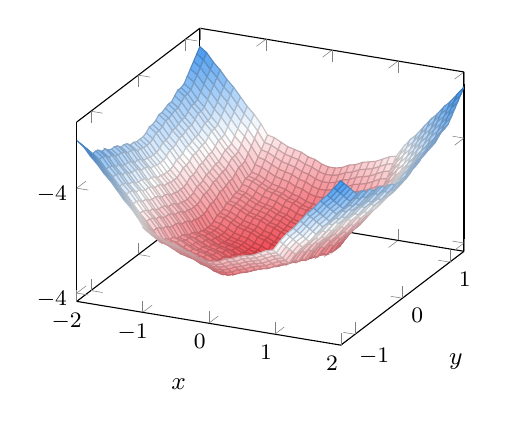
\begin{tikzpicture}[scale=1]
                \begin{axis}[
                    xlabel=$x$, ylabel=$y$,
                    small,
                    colormap name=cool
                ]
                \addplot3[
                    surf,
                    samples=40,
                    domain=-2:2,
                    domain y=-1.3:1.3,
                ] 
                    {-(cos(x)^2+cos(y)^2)^2};
                \end{axis}
            \end{tikzpicture}
            \captionof{figure}{Gradient in a 3D scalar field.}
            \label{img:tikz:rendering:gradient3d}
        \end{minipage}
\end{figure}


\noindent
Mathematically, the \gls{gradient} of a function $f$ at point $p=(x,y,z)$ defines the direction to move in from $p$ to most rapidly increase the value of $f$. 
It is written as $\nabla f$.
$$
\nabla f = \left( \frac{\partial f}{\partial x}, \frac{\partial f}{\partial y}, \frac{\partial f}{\partial z} \right)
$$

\noindent
Instead of calculating the real derivative of the SDF, an approximation is used to estimate the normal vectors.
As previously declared, the \gls{sdf} returns zero for a point on the surface, greater than zero if the point is outside and less than zero if it is inside the volume. 
Therefore, the direction at the surface which will go from negative to positive most quickly will be orthogonal to the surface.
\\
\begin{minipage}{\linewidth}
The estimation $\overrightarrow{n}$ is done by sampling some points around the point on the surface and take their difference, the result of which is the approximate \gls{surfacenormal}.
$$
\overrightarrow{n} = 
\left[
    \begin{matrix}
        f(x + \epsilon, y, z) - f(x - \epsilon, y, z) \\
        f(x, y + \epsilon, z) - f(x, y - \epsilon, z) \\
        f(x, y, z + \epsilon) - f(x, y, z - \epsilon)
       \end{matrix}
\right]
$$

\noindent
The implementation of surface normal estimation looks like this:

\begin{lstlisting}[language=HLSL, caption=Implementation of surface normal estimation., label=lst:shader:surfacenormal]
float3 estimateNormal(float3 p) {
  return normalize(float3(
    sceneSDF(p + float3(EPSILON,0,0)) - sceneSDF(p - float3(EPSILON,0,0)),
    sceneSDF(p + float3(0,EPSILON,0)) - sceneSDF(p - float3(0,EPSILON,0)),
    sceneSDF(p + float3(0,0,EPSILON)) - sceneSDF(p - float3(0,0,EPSILON)),
  ));
}
\end{lstlisting}
\end{minipage}

\noindent
Now that the normal vectors can be calculated for the volume, the object can be shaded. In this example, the Phong Illumination Model \cite{online:phong} is used. 

\begin{figure}[H]
    \centering
        \begin{minipage}{0.47\linewidth}
            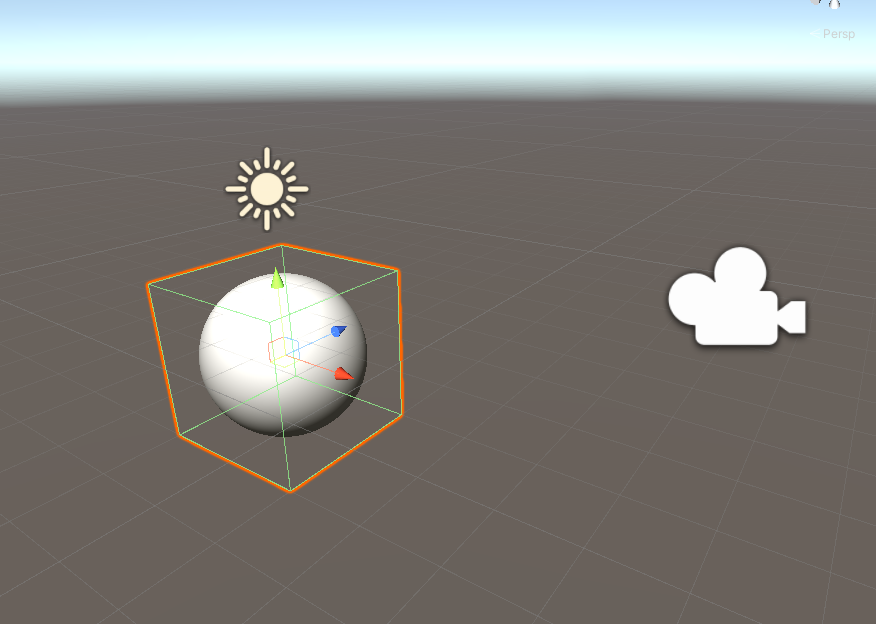
\includegraphics[width=\linewidth]{unity captures/sphere tracing shaded}
            \captionof{figure}{A 3D cube with a volumetric shader.}
            \label{img:captures:spheretracing}
        \end{minipage}
    \hfill
        \begin{minipage}{0.47\linewidth}
            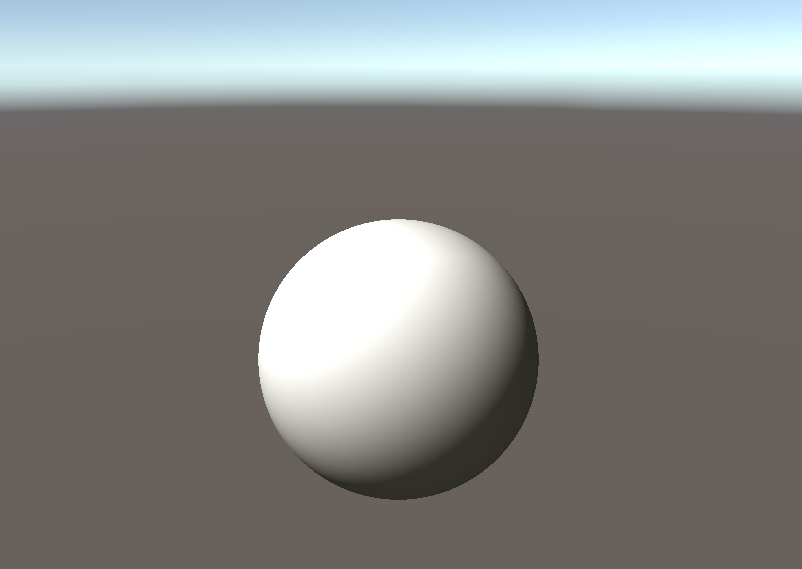
\includegraphics[width=\linewidth]{unity captures/sphere tracing shaded result}
            \captionof{figure}{The shaded sphere rendered volumetrically.}
            \label{img:captures:spheretracing_rendered}
        \end{minipage}
\end{figure}

\clearpage
\subsection{Shadow Casting}
In \gls{raymarching}, rendering hard cast shadows proves to be rather easy. Naturally, the light ray comes from the sun, bounces off in the world and may eventually hit the eye of the observer.
Since only a minute fraction of those rays actually reach the observer (the camera), a huge amount of rays would be calculated for nothing.
Consequently, the rays are not traced from the light source to the camera but the other way around instead.
\\
As defined in \autoref{lst:shader:raymarch:spheretracing}, the \lstinline[language=HLSL]{raymarch()} function moves along the given ray and returns the distance to the intersection point of ray and volume.
Therefore, when a surface point has been determined, a second ray march can be started from the newly found point in the opposite direction of the primary light source's direction.
If anything is hit on the way, the surface point lies in the shadow of the second hit object and should be darkened.

\begin{figure}[H]
    \centering
    \begin{tikzpicture}[scale=1.2]
        \tikzset{edge/.style = {-{Latex[length=3mm]},shorten >= -4pt}}
        \tikzset{shadowedge/.style = {-{Latex[length=3mm]},shorten <=-4pt,shorten >= -4pt}}
        \tikzset{topshadowedge/.style = {-{Latex[length=3mm]},shorten <=-4pt}}
        \tikzset{icon/.style = {font=\Large}}

        % surf dist
        \draw[red] (5,2.5) circle (1);
        \node[red] at (6,3.75) {volume boundary 1};
        \draw[red] (-2,0) -- (7,0) -- (8,0.5);
        \node[red] at (1,0.2) {volume boundary 2};

        \node (rOrigin) at (0.2,2) {};
        \node[cyan] (r1hit) at (4.05,2.8) {\textbullet};
        \node[cyan] (r2hit) at (5.5,0) {\textbullet};
        \node[cyan] (r2light) at (5.35,1.55) {\textbullet};

        % icons
        \node (cam) at (0,2) {\faVideoCamera};
        \node[icon] (light) at (1,5) {\faLightbulbO};
        \node at (1,5.5) {light direction};
        \draw[edge] (light) -- ($ (light) - (-0.11,1) $);
        \draw[edge] ($ (light) + (0.5,0) $) -- ($ (light) + (0.61,-1) $);
        \draw[edge] ($ (light) - (0.5,0) $) -- ($ (light) + (-0.41,-1) $);

        % rays
        \draw[edge] (rOrigin) -- (r1hit) node[midway,above,sloped]{$r1$};
        \draw[topshadowedge, cyan] (r1hit) -- ($ (r1hit) + (-0.16,1.5) $) node[midway,above,sloped]{$s1$};
        
        \draw[edge] (rOrigin) -- (r2hit) node[midway,above,sloped]{$r2$};
        \draw[shadowedge, cyan] (r2hit) -- (r2light) node[midway,above,sloped]{$s2$};
        \draw[loosely dashed, cyan] (r2light) -- ($ (r2light) + (-0.16,1.5) $);

        \end{tikzpicture}
    \captionof{figure}{Shadow casting in ray marching.}
    \label{img:tikz:rendering:shadowcasting}
\end{figure}

\noindent
As seen in the figure above, the ray $r1$ hits the volumetric sphere, then checks if anything is between the ray intersection and the negative light source direction.
In this case, $s1$ does not collide with anything and the surface is shaded normally. 
For the other ray $r2$ however, the shadow ray march returns a distance $s2 > 0$ and $s2 < $\lstinline[language=HLSL]{ MAX_DISTANCE}, meaning some object is in-between the hit point and the light source, casting a shadow.
\\
\begin{lstlisting}[language=HLSL, caption=Implementation of hard shadow casting., label=lst:shader:shadowcasting:hard]
// dMin: minimum distance required for shadow to be cast.
// dMax: maximum distance for shadow casting.
float hardshadow(float3 position, float3 direction, float dMin, float dMax)
{
    float dOrigin = dMin;
    for (int i = 0; i < MAX_STEPS; i++) {
        float dScene = sceneSDF(position + direction * dOrigin);
        if (dScene < SURFACE_DISTANCE)
            return 0.0;
        if (dScene > dMax)
            return 1.0;
        
        dOrigin += dScene;
    }
    return 1.0;
}
\end{lstlisting}

\noindent
It is very clearly similar to SDF-based sphere tracing, except that only 0 or 1 is returned instead of the distance.
The final color is then multiplied by this output. For 0, this results in a total black, hence the name \textit{hard} shadows.

\subsubsection{Soft Shadows}
The method described in \autoref{img:tikz:rendering:shadowcasting} evaluates only if any given point is directly covered by any other object. 
It does not account for diffuse shadows with soft edges, called \textit{\gls{penumbra}} or simply \textit{soft} shadows. But there is an easy and also cost-effective solution to that problem.
Instead of strictly returning 0 when an object is covered by another, the shortest distance to the scene (qualified by some factor $k$) is returned.

\begin{lstlisting}[language=HLSL, caption=Implementation of hard shadow casting., label=lst:shader:shadowcasting:soft]
float softshadow(float3 position, float3 direction, float dMin, float dMax, float k)
{
    float result = 1.0;
    float dOrigin = dMin;
    for (int i = 0; i < MAX_STEPS; i++) {
        float dScene = sceneSDF(position + direction * dOrigin);
        if (dScene < SURFACE_DISTANCE)
            return 0;
        if (dOrigin > dMax)
            return result;
        
        result = min(result, k * dScene / dOrigin);
        dOrigin += dScene;
    }
    return result;
}
\end{lstlisting}

\noindent
Those are the resulting renders with a sphere and a flat box as the volumetric scene.
\begin{figure}[H]
    \centering
        \begin{minipage}{0.3\linewidth}
            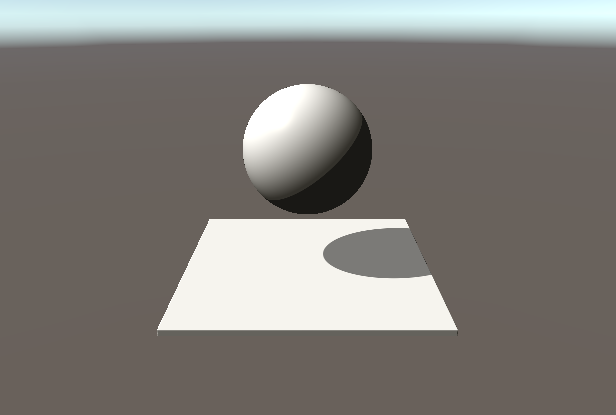
\includegraphics[width=\linewidth]{unity captures/shadow casting hard}
            \captionof{figure}{Hard shadows only.}
            \label{img:captures:shadows:hard}
        \end{minipage}
        \hfill
        \begin{minipage}{0.3\linewidth}
            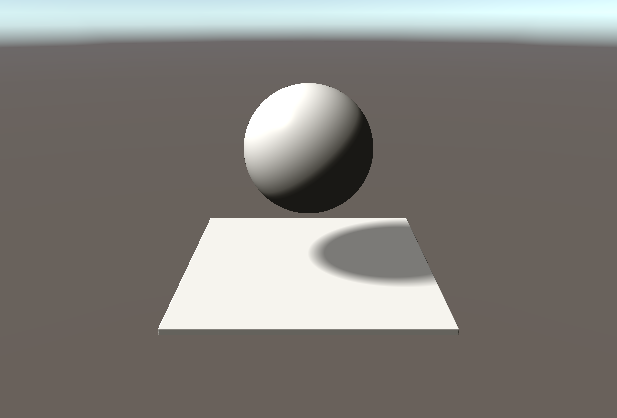
\includegraphics[width=\linewidth]{unity captures/shadow casting soft 7}
            \captionof{figure}{Soft shadows with $k=7.0$.}
            \label{img:captures:shadows:soft2}
        \end{minipage}
        \hfill
        \begin{minipage}{0.3\linewidth}
            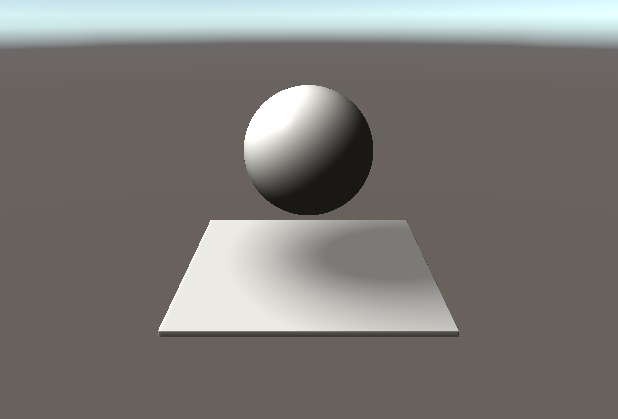
\includegraphics[width=\linewidth]{unity captures/shadow casting soft 1.2}
            \captionof{figure}{Soft shadows with $k=1.2$.}
            \label{img:captures:shadows:soft1}
        \end{minipage}
\end{figure}

\clearpage
\subsection{Shape Blending}
Another thing that comes free with ray marching is \textit{\gls{shapeblending}}. It describes the concept of blending the \gls{sdf}s of multiple shapes together with this simple method:
\begin{lstlisting}[language=HLSL]
// d1: the first SDF.
// d2: the second SDF.
// k:  interpolation factor.
float blend(float d1, float3 d2, float k)
{
    return k * d1 + (1 - k) * d2;
}
\end{lstlisting}

\noindent
Now two shapes can simply be blended like that:
\begin{lstlisting}[language=HLSL]
float sceneSDF(float3 position)
{
    return blend(sphereSDF(position), boxSDF(position), 0.5);
}
\end{lstlisting}

\noindent
The following image displays the two blended shapes. Due to the fact that the shadow calculation is based on the same SDFs, no additional changes have to be made in this regard.
\begin{figure}[H]
    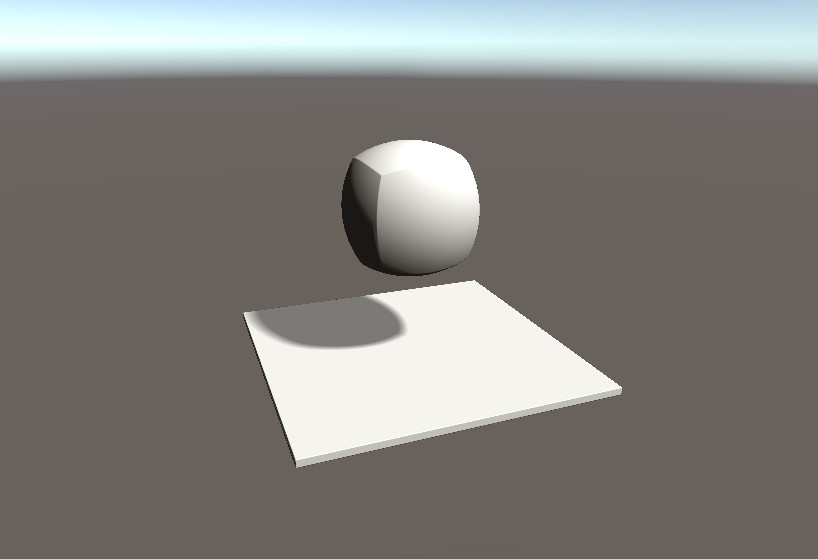
\includegraphics[width=\linewidth]{unity captures/shape blending 1}
    \captionof{figure}{A blended sphere and box SDF with $k = 0.5$.}
    \label{img:captures:shapeblending1}
\end{figure}

\clearpage
\subsubsection{Constructive Solid Geometry}
To create more interesting figures than a rounded box, \gls{csg} (CSG) operators can be used. As seen in \autoref{img:captures:shapeblending2}, "holes" are cut into the geometry. This is done by taking the difference (or intersection) of the box and a cylinder that goes through the box.
Like the \lstinline[language=HLSL]{blend()} function takes in two \gls{sdf} results, the following methods are also based on those values.

\begin{lstlisting}[language=HLSL, caption=Implementation of constructive sold geometry., label=lst:shader:shapeblending:primitiveoperations]
float intersection(float d1, float d2)
{
    return max(d1, d2);
}

float union(float d1, float d2)
{
    return min(d1, d2);
}

float difference(float d1, float d2)
{
    return max(d1, -d2);
}
\end{lstlisting}

\noindent
In this example, the intersection was done three times, for each axis once.

\begin{figure}[H]
    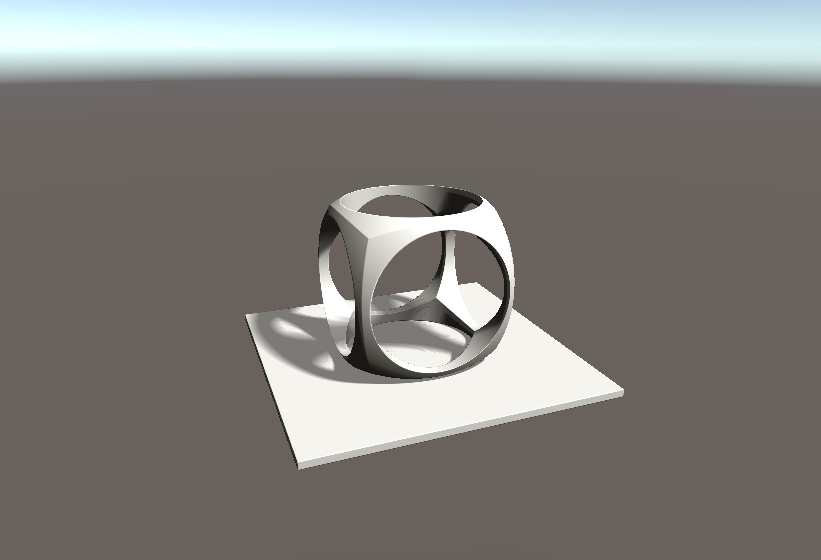
\includegraphics[width=\linewidth]{unity captures/shape blending 2}
    \captionof{figure}{A blended sphere and box with cylinder intersection holes along each axis.}
    \label{img:captures:shapeblending2}
\end{figure}

\clearpage
\subsection{Ambient Occlusion}
Shadow casting already looks quite realistic, but there is an important detail missing, called \textit{\gls{ambientocclusion}}. This method darkens areas around edges and crevices in the scene, making them look less exposed to the light and its environment.
The algorithm for that is fairly uncomplicated and straightforward, given all the previously defined methods like \lstinline[language=HLSL]{sceneSDF()} and \lstinline[language=HLSL]{raymarch()} already exist.
\\
When the \lstinline[language=HLSL]{raymarch()} function returns a valid distance, a surface is hit. On that hit point $p_1$, the normal vector $\overrightarrow{n}$ is estimated. Now the distance to the nearest surface in the direction of $\overrightarrow{n}$ is evaluated.
If on that ray a hit point $p_2$ is close, the color for the original hit point $p_1$ is darkened by some amount, depending on how far apart those points are.

\begin{lstlisting}[language=HLSL, caption=Implementation of ambient occlusion., label=lst:shader:ambientocclusion]
float ambientOcclusion(float3 p, float3 direction) {
    float ao = 0;
    float dOrigin = 0;

    for (int i = 1; i <= AO_ITERATIONS; i++) {
        dOrigin = AO_STEP_SIZE * i;
        ao += max(0, dOrigin - sceneSDF(p + direction * dOrigin)) / dOrigin;
    }
    return 1 - ao * AO_INTENSITY;
}
\end{lstlisting}

\noindent
This comes close to the constant step ray marching algorithm, since it is marched along the ray in a predefined step size.
On line 7, the scene SDF is substracted from the total distance and then divided by it. This just puts the scene distance in relation to the total distance.
Also, \lstinline[language=HLSL]{max()} is used because the SDF can return a negative number for points inside the surface, so in order to not brighten the scene at point \lstinline[language=HLSL]{p} when this is the case, 0 is used instead.
\\
With \lstinline[language=HLSL]{AO_STEP_SIZE = 0.1}, \lstinline[language=HLSL]{AO_ITERATIONS = 3} and \lstinline[language=HLSL]{AO_INTENSITY = 0.2}, the following output is produced:

\begin{figure}[H]
    \centering
        \begin{minipage}{0.47\linewidth}
            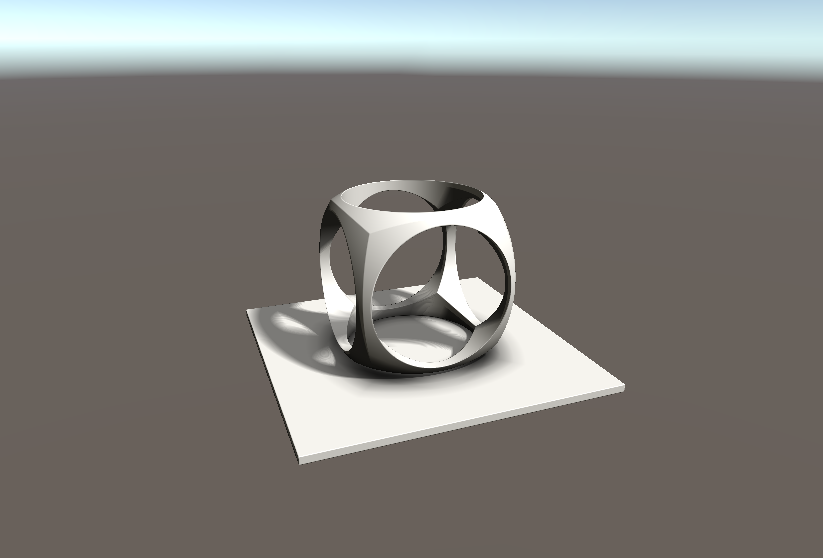
\includegraphics[width=\linewidth]{unity captures/ambient occlusion ON}
            \captionof{figure}{Ambient occlusion applied to the scene.}
            \label{img:captures:ambientocclusion:on}
        \end{minipage}
    \hfill
        \begin{minipage}{0.47\linewidth}
            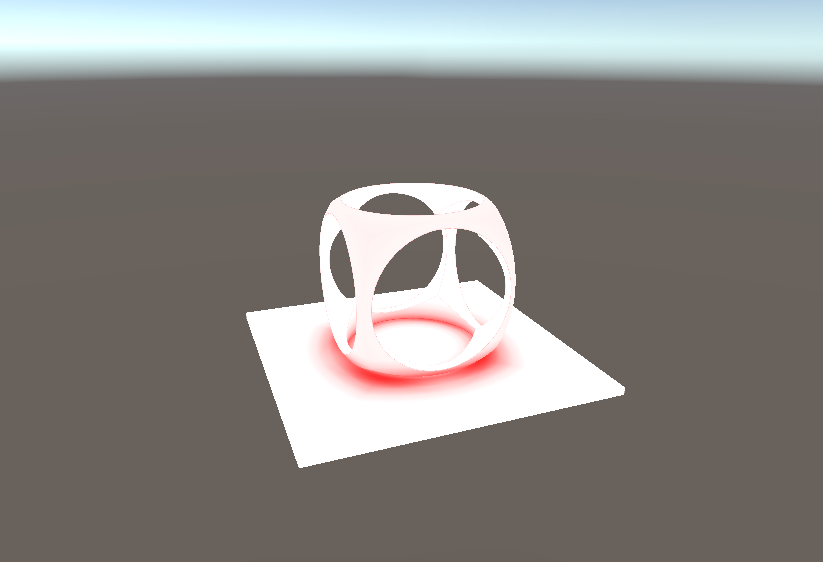
\includegraphics[width=\linewidth]{unity captures/ambient occlusion only}
            \captionof{figure}{Only the ambient occlusion part drawn in red.}
            \label{img:captures:ambientocclusion:only}
        \end{minipage}
\end{figure}

\noindent
When comparing the previous \autoref{img:captures:shapeblending2} with \autoref{img:captures:ambientocclusion:on}, the darker ground around the object clearly improves the scene.
\clearpage

\section{Noise Generation}
\label{section:noise-generation}
Nature's chaotic behavior plays a big role in the diversity and appearance of cloudscapes. In shaders, an approach to simulate \textit{randomness} is using so-called \textit{\gls{noisegeneration}}.
In order to be able to implement random \gls{noisegeneration}, several important topics need to be looked into. It is best to start with randomness in computer science and how it is handled inside a shader program.

\subsection{Random Numbers}
Unfortunately, there is no magic function which returns a purely random number inside the seemingly predictable and deterministic execution environment.
So the question arises as to how such randomness can be generated.
\\
For this, the function $rnd(x) = fract(sin(x))$ is inspected, where $fract(x) = x - floor(x)$.

\begin{figure}[H]
    \centering
    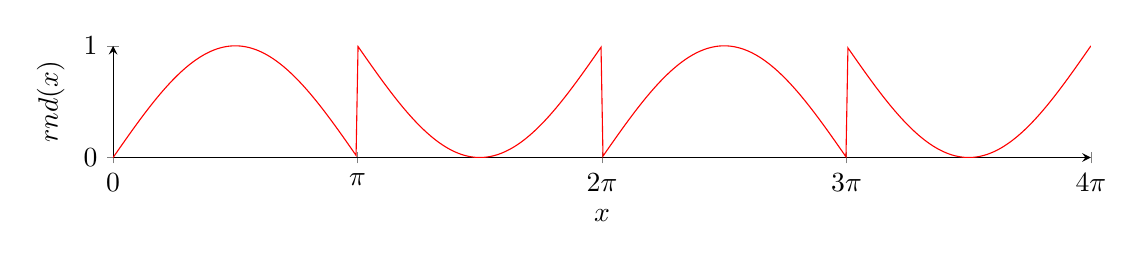
\begin{tikzpicture}[scale=1.0]
        \begin{axis}[
            samples=500,
            domain=0:4*pi,
            axis lines=left,
            xlabel=$x$,
            ylabel={$rnd(x)$},
            height=3cm,
            width=14cm,
            ytick={0,1},
            xtick={0,pi,2*pi,3*pi,4*pi},
            xticklabels={$0$,$\pi$,$2\pi$,$3\pi$,$4\pi$}
            ]
        \addplot[red] plot (\x, { sin(\x*1 r) - floor(sin(\x*1 r)) });
        \end{axis}
    \end{tikzpicture}
    \captionof{figure}{Random numbers with the fractional value of sine of x.}
\end{figure}

\noindent
The sine values fluctuate between $-1.0$ and $1.0$, but with $fract$, only the fractional part is evaluated, turning the negative values into positive ones.
This effect can be used to get some pseudo-random values by "compressing" the function horizontally, or in other words by increasing the frequency of the sine wave.
\\
The next figure displays the function $rnd(x) = fract(sin(x) * 10000)$.

\begin{figure}[H]
    \centering
    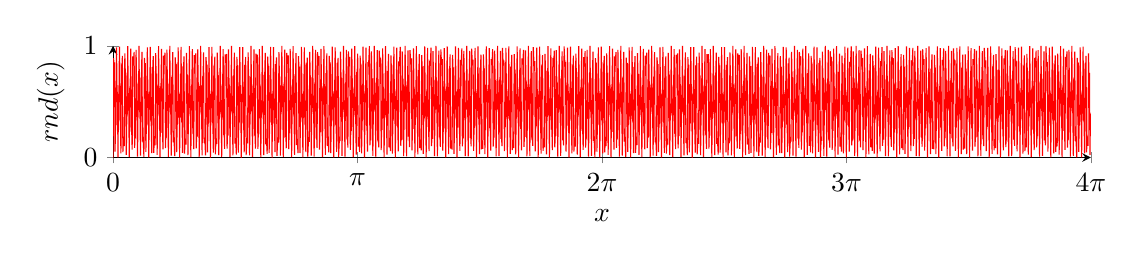
\begin{tikzpicture}[scale=1.0]
        \begin{axis}[
            samples=2000,
            domain=0:4*pi,
            axis lines=left,
            xlabel=$x$,
            ylabel={$rnd(x)$},
            height=3cm,
            width=14cm,
            ytick={0,1},
            xtick={0,pi,2*pi,3*pi,4*pi},
            xticklabels={$0$,$\pi$,$2\pi$,$3\pi$,$4\pi$},
            ]
        \addplot[red] plot (\x, { sin(\x*10000) - floor(sin(\x*10000)) });
        \end{axis}
    \end{tikzpicture}
    \captionof{figure}{Random numbers with the fractional value of sine of x multiplied by 10000.}
\end{figure}

\noindent
It is clearly visible that the function $rnd(x)$ became chaotic and returns practically random values. However, it is noteworthy that $rnd(x)$ is still a deterministic function, which means for example $rnd(1.0)$ is always going to return the same value.

\clearpage
\subsection{2D and 3D Random}
To generate a pseudo-random number from two and three values instead of one, the same function can be used, with some tweaks. Those two numbers come as a two-dimensional vector, which needs to be transformed into a single floating point number.
According to Vivo \cite{online:thebookofshaders}, the dot product is particularly helpful in that case. It returns a single float value between $0.0$ and $1.0$ depending on the alignment of two vectors.
They describe the following methods:

\begin{lstlisting}[language=HLSL, caption=Implementation of 2D random number generation., label=lst:random:2d]
// co: two-dimensional position vector.
float random(float2 co) {
    float2 other = float2(12.9898, 78.233);
    return fract(sin(dot(co, other)) * 43758.5453123);
}
\end{lstlisting}

\begin{lstlisting}[language=HLSL, caption=Implementation of 3D random number generation., label=lst:random:3d]
float random(float3 co) {
    float3 other = float3(12.9898, 78.233, 37.719);
    return fract(sin(dot(co, other)) * 43758.5453123);
}
\end{lstlisting}

\noindent
When using the fragment coordinates as the vector \lstinline[language=HLSL]{co} to call \lstinline[language=HLSL]{random(co)} for every pixels, the resulting image shows a seemingly random assortment of pixels holding values from 0 to 1 (from black to white).

\begin{figure}[H]
    \centering
            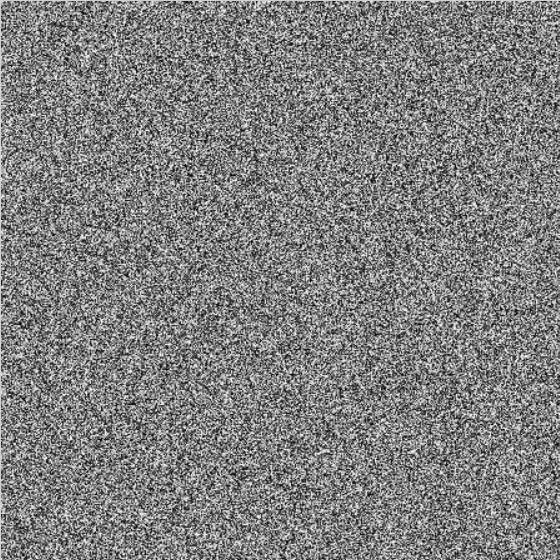
\includegraphics[width=0.45\linewidth]{noise/2d random}
            \captionof{figure}{2D random function visualized.}
            \label{img:noise:2d:random}
\end{figure}

\noindent
This method of \gls{procedural} randomness still has one major flaw: It has no patterns. Contradictory to the word \textit{random}, a certain pattern is required in order to generate \textit{random} clouds. Luckily, there is more to random generation than just a high frequency sine wave.

\clearpage
\subsection{Procedural Noise Patterns}
Now that the concept of random numbers in the world of shaders is no longer a mystery, more advanced noise generation algorithms can be introduced.
When using the word \textit{\gls{noise}} in this context, usually \gls{procedural} pattern generation is meant.

\subsubsection{Perlin Noise}
One of the most commonly used \gls{procedural} pattern generation algorithms is that of Ken Perlin. His algorithm works with the gradient, which was already introduced in \sectionref{section:rendering:surfacenormalestimation}.
\\
It consists of the following three steps: 
\begin{enumerate}
    \item grid definition
    \item dot product calculation between random gradient and distance vectors
    \item interpolation of those dot product values
\end{enumerate}

\noindent
Note that the following example refers to two-dimensional Perlin noise generation, but with some tweaks, is very much applicable for higher dimensional noise generation.
\\
First, the 2D image space is split into a grid. For each vertex or corner point on this grid, a pseudo-random gradient vector is determined.

\begin{figure}[H]
    \centering
        \begin{minipage}{0.47\linewidth}
            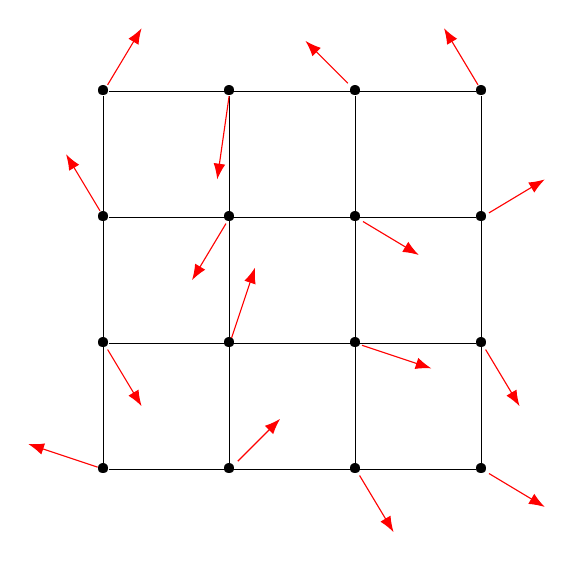
\begin{tikzpicture}[scale=0.8, x=2cm,y=2cm]
                \tikzset{c/.style = {shorten <=-4pt, shorten >=-4pt}}
                \tikzset{smalledge/.style = {-{Latex[length=2mm]},shorten <=-4pt}}
              
                \node (x1y1) at (0,0) {\textbullet};
                \node (x2y1) at (1,0) {\textbullet};
                \node (x3y1) at (2,0) {\textbullet};
                \node (x4y1) at (3,0) {\textbullet};
        
                \node (x1y2) at (0,1) {\textbullet};
                \node (x2y2) at (1,1) {\textbullet};
                \node (x3y2) at (2,1) {\textbullet};
                \node (x4y2) at (3,1) {\textbullet};
        
                \node (x1y3) at (0,2) {\textbullet};
                \node (x2y3) at (1,2) {\textbullet};
                \node (x3y3) at (2,2) {\textbullet};
                \node (x4y3) at (3,2) {\textbullet};
        
                \node (x1y4) at (0,3) {\textbullet};
                \node (x2y4) at (1,3) {\textbullet};
                \node (x3y4) at (2,3) {\textbullet};
                \node (x4y4) at (3,3) {\textbullet};
        
                \draw[c] (x1y1) edge node{} (x4y1);
                \draw[c] (x1y2) edge node{} (x4y2);
                \draw[c] (x1y3) edge node{} (x4y3);
                \draw[c] (x1y4) edge node{} (x4y4);
        
                \draw[c] (x1y1) edge node{} (x1y4);
                \draw[c] (x2y1) edge node{} (x2y4);
                \draw[c] (x3y1) edge node{} (x3y4);
                \draw[c] (x4y1) edge node{} (x4y4);
        
                % arrows
                \draw[smalledge, red] (x1y1) edge node{} ($ (x1y1) + (-0.6,0.2) $);
                \draw[smalledge, red] (x2y1) edge node{} ($ (x2y1) + (0.4,0.4) $);
                \draw[smalledge, red] (x3y1) edge node{} ($ (x3y1) + (0.3,-0.5) $);
                \draw[smalledge, red] (x4y1) edge node{} ($ (x4y1) + (0.5,-0.3) $);
        
                \draw[smalledge, red] (x1y2) edge node{} ($ (x1y2) + (0.3,-0.5) $);
                \draw[smalledge, red] (x2y2) edge node{} ($ (x2y2) + (0.2,0.6) $);
                \draw[smalledge, red] (x3y2) edge node{} ($ (x3y2) + (0.6,-0.2) $);
                \draw[smalledge, red] (x4y2) edge node{} ($ (x4y2) + (0.3,-0.5) $);
        
                \draw[smalledge, red] (x1y3) edge node{} ($ (x1y3) + (-0.3,0.5) $);
                \draw[smalledge, red] (x2y3) edge node{} ($ (x2y3) + (-0.3,-0.5) $);
                \draw[smalledge, red] (x3y3) edge node{} ($ (x3y3) + (0.5,-0.3) $);
                \draw[smalledge, red] (x4y3) edge node{} ($ (x4y3) + (0.5,0.3) $);
        
                \draw[smalledge, red] (x1y4) edge node{} ($ (x1y4) + (0.3,0.5) $);
                \draw[smalledge, red] (x2y4) edge node{} ($ (x2y4) + (-0.1,-0.7) $);
                \draw[smalledge, red] (x3y4) edge node{} ($ (x3y4) + (-0.4,0.4) $);
                \draw[smalledge, red] (x4y4) edge node{} ($ (x4y4) + (-0.3,0.5) $);
        
                \end{tikzpicture}
                \captionof{figure}{Perlin grid with pseudo-random gradient vectors.}
                \label{img:tikz:noise:perlin:gradient}
        \end{minipage}
    \hfill
    \begin{minipage}{0.47\linewidth}
        \begin{tikzpicture}[scale=0.8, x=2cm,y=2cm]
            \tikzset{c/.style = {shorten <=-4pt, shorten >=-4pt}}
            \tikzset{smalledge/.style = {-{Latex[length=2mm]},shorten <=-4pt}}

            \begin{scope}
                \clip (0,0) rectangle (3,3);
                
                \node [shading=axis,rectangle,left color=white, right color=gray,shading angle=180+65,  minimum width=0.8*2cm, minimum height=0.8*2cm] (box) at (x1y1){};
                \node [shading=axis,rectangle,left color=white, right color=gray,shading angle=180-40,  minimum width=0.8*2cm, minimum height=0.8*2cm] (box) at (x2y1){};
                \node [shading=axis,rectangle,left color=white, right color=gray,shading angle=180-145, minimum width=0.8*2cm, minimum height=0.8*2cm] (box) at (x3y1){};
                \node [shading=axis,rectangle,left color=white, right color=gray,shading angle=180-110, minimum width=0.8*2cm, minimum height=0.8*2cm] (box) at (x4y1){};
                
                \node [shading=axis,rectangle,left color=white, right color=gray,shading angle=180-145, minimum width=0.8*2cm, minimum height=0.8*2cm] (box) at (x1y2){};
                \node [shading=axis,rectangle,left color=white, right color=gray,shading angle=180-10,  minimum width=0.8*2cm, minimum height=0.8*2cm] (box) at (x2y2){};
                \node [shading=axis,rectangle,left color=white, right color=gray,shading angle=180-100, minimum width=0.8*2cm, minimum height=0.8*2cm] (box) at (x3y2){};
                \node [shading=axis,rectangle,left color=white, right color=gray,shading angle=180-165, minimum width=0.8*2cm, minimum height=0.8*2cm] (box) at (x4y2){};
                
                \node [shading=axis,rectangle,left color=white, right color=gray,shading angle=180+30,  minimum width=0.8*2cm, minimum height=0.8*2cm] (box) at (x1y3){};
                \node [shading=axis,rectangle,left color=white, right color=gray,shading angle=180+140, minimum width=0.8*2cm, minimum height=0.8*2cm] (box) at (x2y3){};
                \node [shading=axis,rectangle,left color=white, right color=gray,shading angle=180-120, minimum width=0.8*2cm, minimum height=0.8*2cm] (box) at (x3y3){};
                \node [shading=axis,rectangle,left color=white, right color=gray,shading angle=180-55,  minimum width=0.8*2cm, minimum height=0.8*2cm] (box) at (x4y3){};

                \node [shading=axis,rectangle,left color=white, right color=gray,shading angle=180-30,  minimum width=0.8*2cm, minimum height=0.8*2cm] (box) at (x1y4){};
                \node [shading=axis,rectangle,left color=white, right color=gray,shading angle=180+175, minimum width=0.8*2cm, minimum height=0.8*2cm] (box) at (x2y4){};
                \node [shading=axis,rectangle,left color=white, right color=gray,shading angle=180+45,  minimum width=0.8*2cm, minimum height=0.8*2cm] (box) at (x3y4){};
                \node [shading=axis,rectangle,left color=white, right color=gray,shading angle=180+35,  minimum width=0.8*2cm, minimum height=0.8*2cm] (box) at (x4y4){};
            \end{scope}

            \node (x1y1) at (0,0) {\textbullet};
            \node (x2y1) at (1,0) {\textbullet};
            \node (x3y1) at (2,0) {\textbullet};
            \node (x4y1) at (3,0) {\textbullet};
    
            \node (x1y2) at (0,1) {\textbullet};
            \node (x2y2) at (1,1) {\textbullet};
            \node (x3y2) at (2,1) {\textbullet};
            \node (x4y2) at (3,1) {\textbullet};
    
            \node (x1y3) at (0,2) {\textbullet};
            \node (x2y3) at (1,2) {\textbullet};
            \node (x3y3) at (2,2) {\textbullet};
            \node (x4y3) at (3,2) {\textbullet};
    
            \node (x1y4) at (0,3) {\textbullet};
            \node (x2y4) at (1,3) {\textbullet};
            \node (x3y4) at (2,3) {\textbullet};
            \node (x4y4) at (3,3) {\textbullet};
    
            \draw[c] (x1y1) edge node{} (x4y1);
            \draw[c] (x1y2) edge node{} (x4y2);
            \draw[c] (x1y3) edge node{} (x4y3);
            \draw[c] (x1y4) edge node{} (x4y4);
    
            \draw[c] (x1y1) edge node{} (x1y4);
            \draw[c] (x2y1) edge node{} (x2y4);
            \draw[c] (x3y1) edge node{} (x3y4);
            \draw[c] (x4y1) edge node{} (x4y4);
    
            % arrows
            \draw[smalledge, red] (x1y1) edge node{} ($ (x1y1) + (-0.6, 0.2) $);
            \draw[smalledge, red] (x2y1) edge node{} ($ (x2y1) + (0.4,  0.4) $);
            \draw[smalledge, red] (x3y1) edge node{} ($ (x3y1) + (0.3, -0.5) $);
            \draw[smalledge, red] (x4y1) edge node{} ($ (x4y1) + (0.5, -0.3) $);
    
            \draw[smalledge, red] (x1y2) edge node{} ($ (x1y2) + (0.3, -0.5) $);
            \draw[smalledge, red] (x2y2) edge node{} ($ (x2y2) + (0.2,  0.6) $);
            \draw[smalledge, red] (x3y2) edge node{} ($ (x3y2) + (0.6, -0.2) $);
            \draw[smalledge, red] (x4y2) edge node{} ($ (x4y2) + (0.3, -0.5) $);
    
            \draw[smalledge, red] (x1y3) edge node{} ($ (x1y3) + (-0.3, 0.5) $);
            \draw[smalledge, red] (x2y3) edge node{} ($ (x2y3) + (-0.3,-0.5) $);
            \draw[smalledge, red] (x3y3) edge node{} ($ (x3y3) + (0.5, -0.3) $);
            \draw[smalledge, red] (x4y3) edge node{} ($ (x4y3) + (0.5,  0.3) $);
    
            \draw[smalledge, red] (x1y4) edge node{} ($ (x1y4) + (0.3,  0.5) $);
            \draw[smalledge, red] (x2y4) edge node{} ($ (x2y4) + (-0.1,-0.7) $);
            \draw[smalledge, red] (x3y4) edge node{} ($ (x3y4) + (-0.4, 0.4) $);
            \draw[smalledge, red] (x4y4) edge node{} ($ (x4y4) + (-0.3, 0.5) $);
    
            \end{tikzpicture}
            \captionof{figure}{Perlin grid with visualized gradient vectors.}
            \label{img:tikz:noise:perlin:gradient_visualized}
    \end{minipage}
\end{figure}

\clearpage
\noindent
For the next step, it is easier to only inspect a single cell. Given the algorithm currently processes the highlighted pixel $p$ in \autoref{img:tikz:noise:perlin:singlecell}, the next task is to determine the distance vectors from each adjacent corner point to the that pixel.
Note that in $\mathbb{R}^2$, the amount of corners is four, while in $\mathbb{R}^3$, its eight.

\begin{figure}[H]
    \centering
    \begin{minipage}{0.47\linewidth}
        \begin{tikzpicture}[scale=2, x=2cm,y=2cm]
            \tikzset{c/.style = {shorten <=-4pt, shorten >=-4pt}}
            \tikzset{smalledge/.style = {-{Latex[length=2mm]},shorten <=-4pt}}
            
            \node (x1y1) at (0,0) {\textbullet};
            \node (x2y1) at (1,0) {\textbullet};
            \node (x1y2) at (0,1) {\textbullet};
            \node (x2y2) at (1,1) {\textbullet};
    
            \draw[c] (x1y1) edge node{} (x1y2);
            \draw[c] (x1y1) edge node{} (x2y1);
            \draw[c] (x2y2) edge node{} (x2y1);
            \draw[c] (x2y2) edge node{} (x1y2);
    
            \node[cyan] (pixel) at (0.7,0.6) {\textbullet};
            \draw[c, cyan] (pixel) -- (1.1,0.8) -- (1.3,0.8) node[xshift=-0.4cm,above]{pixel $p$};
    
            % arrows
            \draw[smalledge, red] (x1y1) edge node{} ($ (x1y1) + (-0.45,0.15) $);
            \draw[smalledge, red] (x2y1) edge node{} ($ (x2y1) + (0.3,0.3) $);
            \draw[smalledge, red] (x1y2) edge node{} ($ (x1y2) + (0.225,-0.375) $);
            \draw[smalledge, red] (x2y2) edge node{} ($ (x2y2) + (0.15,0.45) $);
    
        \end{tikzpicture}
        \captionof{figure}{Perlin grid cell with gradient vectors.}
        \label{img:tikz:noise:perlin:singlecell}
    \end{minipage}
    \hfill
    \begin{minipage}{0.47\linewidth}
        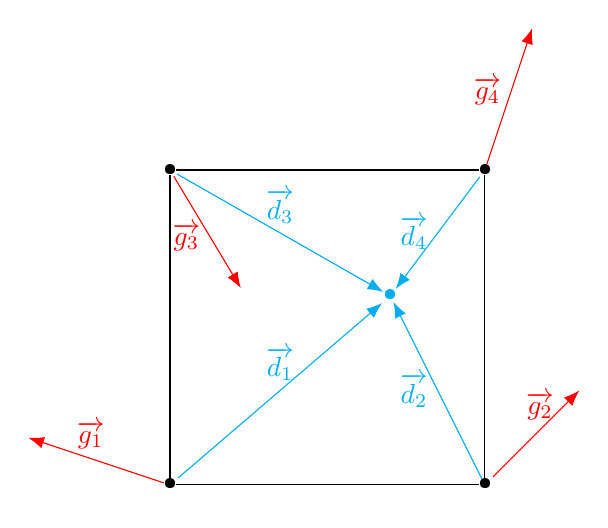
\begin{tikzpicture}[scale=2, x=2cm,y=2cm]
            \tikzset{c/.style = {shorten <=-4pt, shorten >=-4pt}}
            \tikzset{smalledge/.style = {-{Latex[length=2mm]},shorten <=-4pt}}
            
            \node (x1y1) at (0,0) {\textbullet};
            \node (x2y1) at (1,0) {\textbullet};
            \node (x1y2) at (0,1) {\textbullet};
            \node (x2y2) at (1,1) {\textbullet};
    
            \draw[c] (x1y1) edge node{} (x1y2);
            \draw[c] (x1y1) edge node{} (x2y1);
            \draw[c] (x2y2) edge node{} (x2y1);
            \draw[c] (x2y2) edge node{} (x1y2);
    
            \node[cyan] (pixel) at (0.7,0.6) {\textbullet};
    
            % arrows
            \draw[smalledge, red] (x1y1) edge node[above]{$\overrightarrow{g_1}$} ($ (x1y1) + (-0.45,0.15) $);
            \draw[smalledge, red] (x2y1) edge node[above]{$\overrightarrow{g_2}$} ($ (x2y1) + (0.3,0.3) $);
            \draw[smalledge, red] (x1y2) edge node[left] {$\overrightarrow{g_3}$} ($ (x1y2) + (0.225,-0.375) $);
            \draw[smalledge, red] (x2y2) edge node[left] {$\overrightarrow{g_4}$} ($ (x2y2) + (0.15,0.45) $);

            % distance vectors
            \draw[smalledge, cyan, shorten >=-4pt] (x1y1) edge node[above]{$\overrightarrow{d_1}$} (pixel);
            \draw[smalledge, cyan, shorten >=-4pt] (x2y1) edge node[left] {$\overrightarrow{d_2}$} (pixel);
            \draw[smalledge, cyan, shorten >=-4pt] (x1y2) edge node[above]{$\overrightarrow{d_3}$} (pixel);
            \draw[smalledge, cyan, shorten >=-4pt] (x2y2) edge node[left] {$\overrightarrow{d_4}$} (pixel);
    
        \end{tikzpicture}
        \captionof{figure}{Perlin grid cell with distance vectors from each vertex to the pixel.}
        \label{img:tikz:noise:perlin:distancevectors}
    \end{minipage}
\end{figure}

\noindent
Then, the dot product is calculated for each distance vector and its gradient vector. This qualifies how similar those two vectors are, returning a positive number if they face the same direction and a negative one for the opposite. The dot product is 0 if the vectors are perpendicular.
$$ 
\begin{array}{l}
    s = g_1 * d_1,\\
    t = g_2 * d_2,\\
    u = g_3 * d_3,\\
    v = g_4 * d_4.
\end{array}
$$

\noindent
The values $s, t, u, v$ represent the influences of the respective gradient on the final color of the pixel $p$. 
When visualizing those values as vectors with their length being the influence, it looks like this:
\begin{figure}[H]
    \centering
    \begin{tikzpicture}[scale=2, x=2cm,y=2cm]
        \tikzset{c/.style = {shorten <=-6pt, shorten >=-6pt}}
        \tikzset{smalledge/.style = {-{Latex[length=2mm]},shorten <=-6pt}}
        
        \node (x1y1) at (0,0) {\textbullet};
        \node (x2y1) at (1,0) {\textbullet};
        \node (x1y2) at (0.6,0.4) {\textbullet};
        \node (x2y2) at (1.6,0.4) {\textbullet};

        \node[above] at (x1y1) {$S$};
        \node[below] at (x2y1) {$T$};
        \node[below] at (x1y2) {$U$};
        \node[above] at (x2y2) {$V$};

        \draw[c] (x1y1) -- (x1y2);
        \draw[c] (x1y2) -- (x2y2);
        \draw[c] (x2y2) -- (x2y1);
        \draw[c] (x2y1) -- (x1y1);

        % arrows
        \draw[smalledge, red] (x1y1) edge node[left]{$s$} ($(x1y1) + (0,-0.225)$);
        \draw[smalledge, red] (x2y1) edge node[left]{$t$} ($(x2y1) + (0,0.1)$);
        \draw[smalledge, red] (x1y2) edge node[left]{$u$} ($(x1y2) + (0,0.3075)$);
        \draw[smalledge, red] (x2y2) edge node[left]{$v$} ($(x2y2) + (0,-0.225)$);

    \end{tikzpicture}
    \captionof{figure}{Perlin grid cell with visualized influences of gradient vectors.}
    \label{img:tikz:noise:perlin:influences}
\end{figure}

\noindent
\begin{minipage}{\linewidth}
It is clearly recognizable that the color of the pixel is influenced the most by $u$. Now those four numbers can be combined into one final number, the color value.
For that, some sort of average calculation is used. For $\mathbb{R}^2$, the following ruleset applies:

\begin{enumerate}
    \item find the average of the first pair of numbers
    \item find the average of the second pair of numbers
    \item average those two numbers together
\end{enumerate}
\end{minipage}
\vspace{\baselineskip}

\noindent
To get an accurate mean value of those influences, rather than using the arithmetic average, a weighted average calculation is used. The weight for that is how close $p$ is to the vertices.
This means if $p$ is close to a corner point, the influence of that vertex should be weighted heavier than the influences of all other corner points.
\\
This is solved by linear interpolation.
$$
\begin{array}{l}
    d_x = (T_x - p_x) / (T_x) - (S_x),\\
    d_y = (U_y - p_y) / (U_y) - (S_y).\\
    \\
    w_1 = lerp(u, v, d_x),\\
    w_2 = lerp(s, t, d_x),\\
    w_{final} = lerp(w_1, w_2, d_y).
\end{array}
$$

\noindent
Both variables $d_x$ and $d_y$ represent the interpolation weight, being between 0 and 1. With $w_1$, the interpolation between $s$ and $t$ is done, depending on how far to the right the pixel is, related to its cell.
This results in the first interpolation of the X-axis. Now $w_2$ is calculated, giving the second horizontal value in-between $u$ and $v$.
Finally, both $w_1$ and $w_2$ are linearly interpolated in relation to $d_y$, which gives the final average number.


\begin{figure}[H]
    \centering
    \begin{minipage}{0.47\linewidth}
        \centering
        \begin{tikzpicture}[scale=2, x=2cm,y=2cm]
            \tikzset{c/.style = {shorten <=-4pt, shorten >=-4pt}}
            \tikzset{smalledge/.style = {-{Latex[length=2mm]},shorten <=-4pt}}
            
            \node (x1y1) at (0,0) {\small\textbullet};
            \node (x2y1) at (1,0) {\small\textbullet};
            \node (x1y2) at (0,1) {\small\textbullet};
            \node (x2y2) at (1,1) {\small\textbullet};
    
            \draw[c] (x1y1) edge node{} (x1y2);
            \draw[c, red] (x1y1) edge node{} (x2y1);
            \draw[c] (x2y1) edge node{} (x2y2);
            \draw[c, red] (x1y2) edge node{} (x2y2);
    
            \node[cyan] (pixel) at (0.7,0.6) {\textbullet};
            
            % interpolations
            \node[red] (w1) at (0.7,1) {\textbullet};
            \node[red] (w2) at (0.7,0) {\textbullet};
            \draw[c, cyan] (w1) -- (w2) node{};
            \draw[c, red] (w1) node[yshift=.1cm,above]{$w_1$};
            \draw[c, red] (w2) node[yshift=-.1cm,below]{$w_2$};
            \draw[c, cyan] (pixel) node[xshift=-.1cm,left]{$w_{final}$};

        \end{tikzpicture}
        \captionof{figure}{Perlin vertex weights in 2D space with four corners and three interpolations.}
        \label{img:tikz:noise:perlin:interpolation2d}  
    \end{minipage}
    \hfill
    \begin{minipage}{0.47\linewidth}
        \centering
        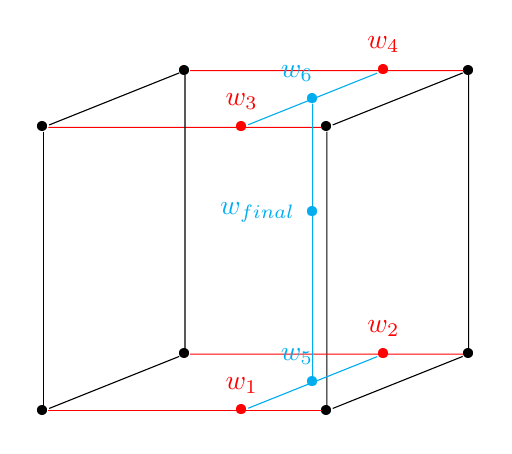
\begin{tikzpicture}[scale=1.8, x=2cm,y=2cm]
            \tikzset{c/.style = {shorten <=-4pt, shorten >=-4pt}}
            \tikzset{smalledge/.style = {-{Latex[length=2mm]},shorten <=-4pt}}
            
            \node (x1y1z1) at (0,0) {\small\textbullet};
            \node (x2y1z1) at (1,0) {\small\textbullet};
            \node (x1y2z1) at (0,1) {\small\textbullet};
            \node (x2y2z1) at (1,1) {\small\textbullet};
            \node (x1y1z2) at (0.5,0.2) {\small\textbullet};
            \node (x2y1z2) at (1.5,0.2) {\small\textbullet};
            \node (x1y2z2) at (0.5,1.2) {\small\textbullet};
            \node (x2y2z2) at (1.5,1.2) {\small\textbullet};
            
            \draw[c,red] (x1y1z1) -- (x2y1z1);
            \draw[c] (x2y1z1) -- (x2y2z1);
            \draw[c,red] (x2y2z1) -- (x1y2z1);
            \draw[c] (x1y2z1) -- (x1y1z1);

            \draw[c,red] (x1y1z2) -- (x2y1z2);
            \draw[c] (x2y1z2) -- (x2y2z2);
            \draw[c,red] (x2y2z2) -- (x1y2z2);
            \draw[c] (x1y2z2) -- (x1y1z2);

            \draw[c] (x1y1z1) -- (x1y1z2);
            \draw[c] (x1y2z1) -- (x1y2z2);
            \draw[c] (x2y1z1) -- (x2y1z2);
            \draw[c] (x2y2z1) -- (x2y2z2);

            % interpolations
            \node[red] (w1) at (0.7,0) {\textbullet};
            \node[red] (w2) at (1.2,0.2) {\textbullet};
            \node[red] (w3) at (0.7,1) {\textbullet};
            \node[red] (w4) at (1.2,1.2) {\textbullet};

            \draw[c,cyan] (w1) -- (w2);
            \draw[c,cyan] (w3) -- (w4);

            \node[cyan] (w5) at (0.95,0.1) {\textbullet};
            \node[cyan] (w6) at (0.95,1.1) {\textbullet};
            \node[cyan] (wfinal) at (0.95,0.7) {\textbullet};

            \draw[c,cyan] (w5) -- (w6);

            \draw[c, red] (w1) node[yshift=.1cm,above]{$w_1$};
            \draw[c, red] (w2) node[yshift=.1cm,above]{$w_2$};
            \draw[c, red] (w3) node[yshift=.1cm,above]{$w_3$};
            \draw[c, red] (w4) node[yshift=.1cm,above]{$w_4$};
            \draw[c, cyan] (w5) node[yshift=.1cm,xshift=-.2cm,above]{$w_5$};
            \draw[c, cyan] (w6) node[yshift=.1cm,xshift=-.2cm,above]{$w_6$};

            \draw[c, cyan] (wfinal) node[xshift=-.1cm,left]{$w_{final}$};

        \end{tikzpicture}
        \captionof{figure}{Perlin vertex weights in 3D space with eight corners and seven interpolations.}
        \label{img:tikz:noise:perlin:interpolation3d}    
    \end{minipage}
    
\end{figure}

\begin{figure}[H]
    \centering
        \begin{minipage}{0.47\linewidth}
            \includegraphics[width=\linewidth]{noise/2D perlin unfaded}
            \captionof{figure}{2D Perlin noise texture with a 10x10 grid.}
            \label{img:noise:perlin:2d_unfaded}
        \end{minipage}
    \hfill
        \begin{minipage}{0.47\linewidth}
            \includegraphics[width=\linewidth]{noise/2D perlin}
            \captionof{figure}{2D Perlin noise texture with Perlin's fade function.}
            \label{img:noise:perlin:2d}
        \end{minipage}
\end{figure}

\noindent
By default, the Perlin noise texture shows a significant amount of artifacts along the grid lines. This can be fixed by using Perlin's fade function \cite{online:perlin:impl} for $d_x$ and $d_y$, which is defined by $f(t) = 6t^5-15t^4+10t^3$.
\emptyline
For 3D, Perlin describes that rather than calculating random gradient vectors, a simple set of 12 distinct vectors can be used, which still provides sufficient randomness but is faster \cite{online:perlin:improved}.
For each grid corner, a hash function is used to generate an index (from 0 to 11), with which one of the gradient vectors is then chosen.


\clearpage
\subsubsection{Voronoi Noise}
While Perlin's noise algorithm is heavy on vector calculation and interpolation, other noise patterns are less complex to understand and construct, like the \textit{Voronoi} noise, also known as \textit{Worley} or \textit{cellular} noise.
The name derives from its similar structure to a Voronoi diagram, in which points, called \textit{seeds}, are randomly scattered inside a defined space. After that, regions are created, consisting of all points closer to that seed than to any other.
\emptyline
As for the noise pattern, there are some alterations. To get a more even distribution, the noise algorithm starts by dividing the space into a grid, for which each cell is assigned a random point. From there, each fragment gets colored by how far it is to the seed in its cell.

\begin{figure}[H]
    \centering

    \begin{minipage}{0.47\linewidth}
        \centering
        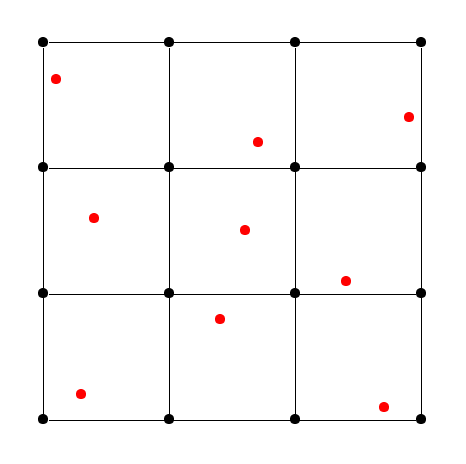
\begin{tikzpicture}[scale=0.8, x=2cm,y=2cm]
        \tikzset{c/.style = {shorten <=-4pt, shorten >=-4pt}}
        \tikzset{smalledge/.style = {-{Latex[length=2mm]},shorten <=-4pt}}
        
        \node (x1y1) at (0,0) {\textbullet};
        \node (x2y1) at (1,0) {\textbullet};
        \node (x3y1) at (2,0) {\textbullet};
        \node (x4y1) at (3,0) {\textbullet};

        \node (x1y2) at (0,1) {\textbullet};
        \node (x2y2) at (1,1) {\textbullet};
        \node (x3y2) at (2,1) {\textbullet};
        \node (x4y2) at (3,1) {\textbullet};

        \node (x1y3) at (0,2) {\textbullet};
        \node (x2y3) at (1,2) {\textbullet};
        \node (x3y3) at (2,2) {\textbullet};
        \node (x4y3) at (3,2) {\textbullet};

        \node (x1y4) at (0,3) {\textbullet};
        \node (x2y4) at (1,3) {\textbullet};
        \node (x3y4) at (2,3) {\textbullet};
        \node (x4y4) at (3,3) {\textbullet};

        \draw[c] (x1y1) edge node{} (x4y1);
        \draw[c] (x1y2) edge node{} (x4y2);
        \draw[c] (x1y3) edge node{} (x4y3);
        \draw[c] (x1y4) edge node{} (x4y4);

        \draw[c] (x1y1) edge node{} (x1y4);
        \draw[c] (x2y1) edge node{} (x2y4);
        \draw[c] (x3y1) edge node{} (x3y4);
        \draw[c] (x4y1) edge node{} (x4y4);

        \node[red] (s1) at (0.3,0.2) {\textbullet};
        \node[red] (s2) at (1.4,0.8) {\textbullet};
        \node[red] (s3) at (2.7,0.1) {\textbullet};
        \node[red] (s4) at (0.4,1.6) {\textbullet};
        \node[red] (s5) at (1.6,1.5) {\textbullet};
        \node[red] (s6) at (2.4,1.1) {\textbullet};
        \node[red] (s7) at (0.1,2.7) {\textbullet};
        \node[red] (s8) at (1.7,2.2) {\textbullet};
        \node[red] (s9) at (2.9,2.4) {\textbullet};

        \end{tikzpicture}
        \captionof{figure}{Voronoi grid with pseudo-randomly assigned seed points for each cell.}
        \label{img:tikz:noise:voronoi}
    \end{minipage}
    \hfill
    \begin{minipage}{0.47\linewidth}
        \centering
        \begin{tikzpicture}[scale=0.8, x=2cm,y=2cm]
            \tikzset{c/.style = {shorten <=-4pt, shorten >=-4pt}}
            \tikzset{smalledge/.style = {-{Latex[length=2mm]},shorten <=-4pt}}
            
            \node (gradient) at (1.5,1.5) {
\includegraphics[width=4.8cm] {noise/2d voronoi unmixed}};

            \node (x1y1) at (0,0) {\textbullet};
            \node (x2y1) at (1,0) {\textbullet};
            \node (x3y1) at (2,0) {\textbullet};
            \node (x4y1) at (3,0) {\textbullet};

            \node (x1y2) at (0,1) {\textbullet};
            \node (x2y2) at (1,1) {\textbullet};
            \node (x3y2) at (2,1) {\textbullet};
            \node (x4y2) at (3,1) {\textbullet};

            \node (x1y3) at (0,2) {\textbullet};
            \node (x2y3) at (1,2) {\textbullet};
            \node (x3y3) at (2,2) {\textbullet};
            \node (x4y3) at (3,2) {\textbullet};

            \node (x1y4) at (0,3) {\textbullet};
            \node (x2y4) at (1,3) {\textbullet};
            \node (x3y4) at (2,3) {\textbullet};
            \node (x4y4) at (3,3) {\textbullet};

            \draw[c] (x1y1) edge node{} (x4y1);
            \draw[c] (x1y2) edge node{} (x4y2);
            \draw[c] (x1y3) edge node{} (x4y3);
            \draw[c] (x1y4) edge node{} (x4y4);

            \draw[c] (x1y1) edge node{} (x1y4);
            \draw[c] (x2y1) edge node{} (x2y4);
            \draw[c] (x3y1) edge node{} (x3y4);
            \draw[c] (x4y1) edge node{} (x4y4);

            \node[red] (s1) at (0.3,0.2) {\textbullet};
            \node[red] (s2) at (1.4,0.8) {\textbullet};
            \node[red] (s3) at (2.7,0.1) {\textbullet};
            \node[red] (s4) at (0.4,1.6) {\textbullet};
            \node[red] (s5) at (1.6,1.5) {\textbullet};
            \node[red] (s6) at (2.4,1.1) {\textbullet};
            \node[red] (s7) at (0.1,2.7) {\textbullet};
            \node[red] (s8) at (1.7,2.2) {\textbullet};
            \node[red] (s9) at (2.9,2.4) {\textbullet};

        \end{tikzpicture}
        \captionof{figure}{Voronoi grid with seed distances visualized.}
        \label{img:tikz:noise:voronoi2}
    \end{minipage}
\end{figure}

\noindent
As understandable, in \autoref{img:tikz:noise:voronoi2}, hard contours are still visible along the grid lines. This can be improved by including the adjacent cells when finding the closest seed for any given fragment.
This amounts to $3^n - 1$ neighboring cells, where $n$ is the number of dimensions. This means for 2D space its eight cells, while in 3D its 26.

\begin{figure}[H]
    \centering
    \begin{tikzpicture}[scale=1.2, x=2cm,y=2cm]
        \tikzset{c/.style = {shorten <=-4pt, shorten >=-4pt}}
        \tikzset{smalledge/.style = {-{Latex[length=2mm]},shorten <=-4pt}}
        
        \node (gradient) at (1.5,1.5) {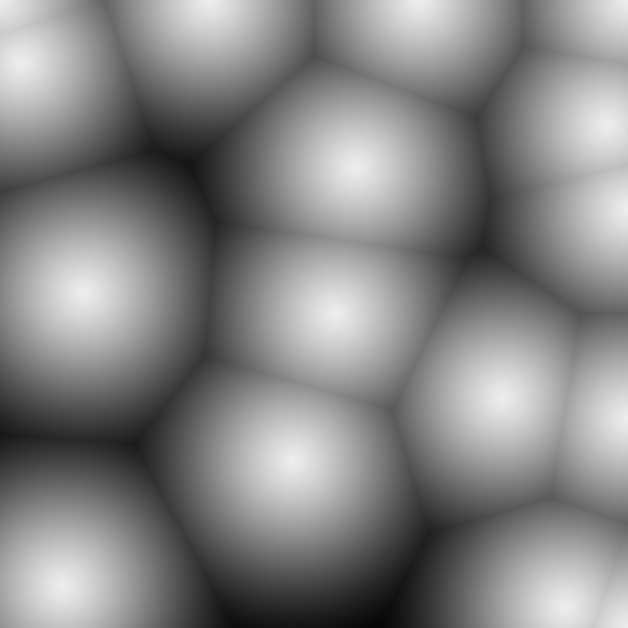
\includegraphics[width=7.2cm] {noise/2d voronoi}};

        \node (x1y1) at (0,0) {\textbullet};
        \node (x2y1) at (1,0) {\textbullet};
        \node (x3y1) at (2,0) {\textbullet};
        \node (x4y1) at (3,0) {\textbullet};

        \node (x1y2) at (0,1) {\textbullet};
        \node (x2y2) at (1,1) {\textbullet};
        \node (x3y2) at (2,1) {\textbullet};
        \node (x4y2) at (3,1) {\textbullet};

        \node (x1y3) at (0,2) {\textbullet};
        \node (x2y3) at (1,2) {\textbullet};
        \node (x3y3) at (2,2) {\textbullet};
        \node (x4y3) at (3,2) {\textbullet};

        \node (x1y4) at (0,3) {\textbullet};
        \node (x2y4) at (1,3) {\textbullet};
        \node (x3y4) at (2,3) {\textbullet};
        \node (x4y4) at (3,3) {\textbullet};

        \draw[c] (x1y1) edge node{} (x4y1);
        \draw[c] (x1y2) edge node{} (x4y2);
        \draw[c] (x1y3) edge node{} (x4y3);
        \draw[c] (x1y4) edge node{} (x4y4);

        \draw[c] (x1y1) edge node{} (x1y4);
        \draw[c] (x2y1) edge node{} (x2y4);
        \draw[c] (x3y1) edge node{} (x3y4);
        \draw[c] (x4y1) edge node{} (x4y4);

        \node[red] (s1) at (0.3,0.2) {\textbullet};
        \node[red] (s2) at (1.4,0.8) {\textbullet};
        \node[red] (s3) at (2.7,0.1) {\textbullet};
        \node[red] (s4) at (0.4,1.6) {\textbullet};
        \node[red] (s5) at (1.6,1.5) {\textbullet};
        \node[red] (s6) at (2.4,1.1) {\textbullet};
        \node[red] (s7) at (0.1,2.7) {\textbullet};
        \node[red] (s8) at (1.7,2.2) {\textbullet};
        \node[red] (s9) at (2.9,2.4) {\textbullet};

    \end{tikzpicture}
    \captionof{figure}{Complete 2D Voronoi noise pattern.}
    \label{img:tikz:noise:voronoi3}
\end{figure}

\noindent
An implementation of this relatively simple algorithm could look like the following listing.
\lstinline[language=HLSL]{randomSeed()} is used like the previously introduced function \lstinline[language=HLSL]{random()}, except that it returns a two-dimensional vector instead of a scalar.
With that, a deterministically random point can be generated for any given cell.

\begin{lstlisting}[language=HLSL, caption=Implementation of 2D Voronoi noise algorithm., label=lst:shader:noise:voronoi2d]
float2 randomSeed(float2 co) {
    return float2(
        fract(sin(dot(co, float2(12.9898, 78.233))) * 43758.5453123),
        fract(sin(dot(co, float2(39.3461, 11.135))) * 14375.8545359));
}

float voronoi(float2 p) {
    float2 pCell = floor(p);
    float dMin = 999;

    for(int x = -1; x <= 1; x++) {
        for(int y = -1; y <= 1; y++) {
            float2 cell = pCell + float2(x, y);
            float2 seed = cell + randomSeed(cell);
            float d = distance(seed, p);
            if (d < dMin) {
                dMin = d;
            }
        }
    }
    
    return dMin;
}
\end{lstlisting}

\noindent
Since the Voronoi noise algorithm creates a cellular pattern, it is well suitable for simulating natural distribution of cloud heaps, as they are in some way also formed "in cells".

\clearpage
\subsubsection{Fractal Brownian Motion}
In the world of shaders, the term \textit{\gls{fbm}} (fBm) is often described as adding different levels of noise together, thus creating a self-similar pattern across different scales \cite{online:thebookofshaders:fractal}.
This simplified description meets the required level of detail for this section, a complete explanation and derivation of the fractal Brownian motion is beyond the scope of this paper.
\emptyline
In shaders, fBms are also called \textit{\gls{fractalnoise}}. They are usually implemented by adding different iterations of noise (called \textit{octaves}), while successively incrementing the frequencies in regular steps (\textit{lacunarity}) and decreasing the amplitude (\textit{gain}) of the noise.
This results in a more detailed noise, meaning a finer granularity of the pattern in the noise.

\begin{lstlisting}[language=HLSL, caption=Implementation of fractal Brownian motion function., label=lst:shader:fbm]
#define LACUNARITY 2.0
#define GAIN 0.5
#define OCTAVES 1
    
float fbm(float2 p) {
    float frequency = 1.0;
    float amplitude = 0.5;
    
    float total = 0;
    float maxValue = 0;
    for(int i = 0; i < OCTAVES; i++) {
        float current = noise(p * frequency) * amplitude;
        total += current;
        maxValue += amplitude;
        
        amplitude *= GAIN;
        frequency *= LACUNARITY;
    }
    
    return total/maxValue;
}
\end{lstlisting}

\noindent
Interestingly, the only things that change for 3D is \lstinline[language=HLSL]{float2 p} becomes a \lstinline[language=HLSL]{float3 p} and the \lstinline[language=HLSL]{noise()} function must accept a three-dimensional vector instead. That's all.
\\
Here are some example images of the fractal Brownian motion with different octaves. For the noise function, a Voronoi noise algorithm was used.
\begin{figure}[H]
    \centering
        \begin{minipage}{0.3\linewidth}
            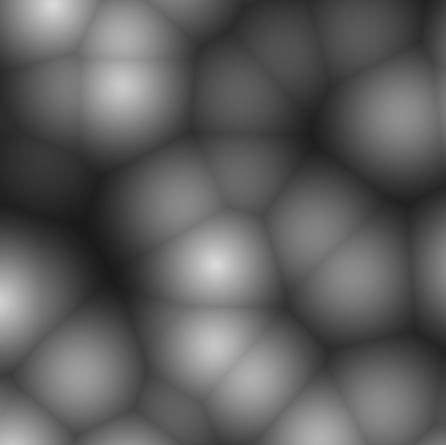
\includegraphics[width=\linewidth]{noise/fbm1}
            \captionof{figure}{One octave of a 2D Voronoi noise.}
            \label{img:noise:fbm1}
        \end{minipage}
        \hfill
        \begin{minipage}{0.3\linewidth}
            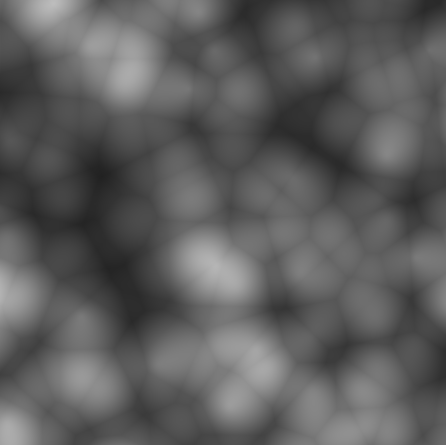
\includegraphics[width=\linewidth]{noise/fbm2}
            \captionof{figure}{Two octaves of a 2D Voronoi noise.}
            \label{img:noise:fbm2}
            \end{minipage}
        \hfill
        \begin{minipage}{0.3\linewidth}
            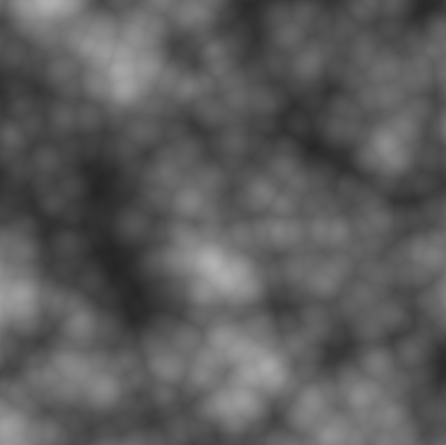
\includegraphics[width=\linewidth]{noise/fbm3}
            \captionof{figure}{Three octaves of a 2D Voronoi noise.}
            \label{img:noise:fbm6}
        \end{minipage}
\end{figure}

\noindent
It is understandable that with every additional octave, the algorithm has to evaluate the noise at all points again, making it worth considering the impact on performance \gls{fractalnoise} has.
However, the final renders look convincingly "cloudy".

\begin{figure}[H]
    \centering
        \begin{minipage}{0.47\linewidth}
            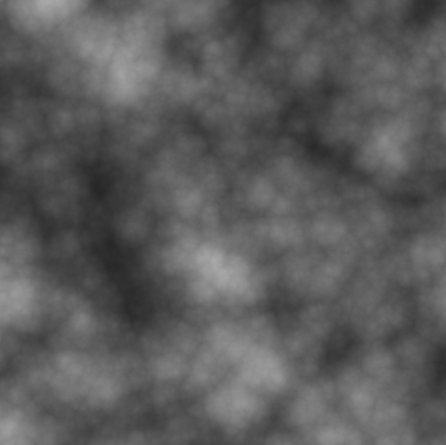
\includegraphics[width=\linewidth]{noise/fbm10_1}
            \captionof{figure}{Ten octaves of a 2D Voronoi noise.}
            \label{img:noise:fbm10_1}
        \end{minipage}
    \hfill
        \begin{minipage}{0.47\linewidth}
            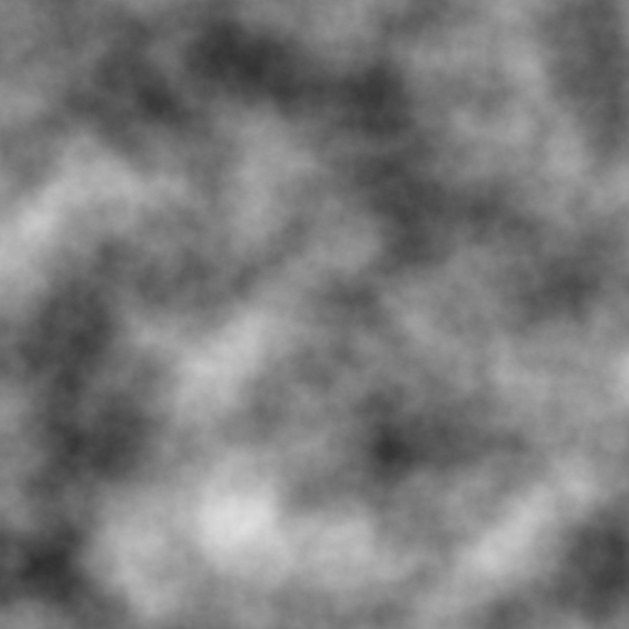
\includegraphics[width=\linewidth]{noise/fbm10_2}
            \captionof{figure}{Ten octaves of a 2D Perlin noise.}
            \label{img:noise:fbm10_2}
        \end{minipage}
\end{figure}
\clearpage

\section{Prototypes and Results}

\subsection{Disclaimer}
\subsubsection{Completed Prototypes}
While researching the topic and experimenting with some dummy shaders, it came clear that "\gls{volumetricrendering}" and "\gls{raymarching}" are interchangeable in this matter.
Therefore, only two kinds of prototyping have been developed. This change is explained in detail in \sectionref{section:projectmanagement:goals}.

\subsubsection{Dimensions}
All of the following documented procedures and algorithms were prototyped and implemented in 3D, but for the matter of explanation, it is described and visualized in 2D.

\subsubsection{Unity Variables}
The following sections will list code snippets, in which all variables prefixed with an underscore are shader variables exposed to the Unity Editor. This way, they can be changed externally while running the shader code, allowing for convenient debugging.
They are from here on out referred to as \textit{\gls{parameters}}.

\clearpage
\subsection{First Draft}
The first drafts of prototypes created during this project all revolve around volumetric rendering. 
Instead of using a \gls{sdf} and evaluating the distance each step, a noise function was used to simulate the \textit{mass} of the cloud. 
The primary issue was to get the cube transparent where the noise function would return a number close to 0.0 and to color it where the number would be close to 1.0.
The approach for solving this issue is done by sampling the cloud's density.

\subsubsection{Density sampling}
Like in \gls{volumetricrendering}, for each pixel fragment, a ray is cast from the fragment into the cube and extended along the view direction for that fragment.
Usually, the algorithm can stop for a given ray if the \gls{sdf} returns a small enough distance, meaning the ray has hit a surface of the volume. However, it is different in the case with clouds, where the volume is \textit{\gls{translucent}} at most points.
\\
To account for that, the ray does not stop until the end of the container cube is reached. It samples the density $N$ times along its path and returns the sum of those samples, giving an approximate qualifier for how dark this fragment should be.

\begin{figure}[H]
    \centering
    \begin{tikzpicture}[scale=1.2]
        \tikzset{edge/.style = {-{Latex[length=3mm]},shorten >= -4pt}}
        \tikzset{shortedge/.style = {-{Latex[length=3mm]},shorten <=-4pt,shorten >= -4pt}}
        \tikzset{icon/.style = {font=\Large}}

        % icons
        \node[icon,rotate=35,anchor=west] (cam) at (0, 0) {\faVideoCamera};

        % clouds
        \node[cloud, cloud puffs=15.7, minimum width=5cm, minimum height=3.5cm, align=center, draw] (cloud) at (4.5, 3.5) {};
        \node[cloud, cloud puffs=15.7, minimum width=2cm, minimum height=1.5cm, align=center, draw] (cloud) at (5.0, 1.1) {};
        \node[cloud, cloud puffs=15.7, minimum width=3cm, minimum height=2.0cm, align=center, draw] (cloud) at (0.2, 3.5) {};
        \node[cloud, cloud puffs=15.7, minimum width=1.5cm,minimum height= 1cm, align=center, draw] (cloud) at (1.75, 0.9) {};

        % outer point
        \node (pOut) at (7, 5.25) {};
        \draw[red, edge] (cam) -- (pOut) node[midway,above,sloped,xshift=-3cm] {};

        % cloud points
        \node[red] (p1) at (1.5, 1.125) {\textbullet};
        \node (p2) at (2.5, 1.875) {\textopenbullet};
        \node[red] (p3) at (3.5, 2.625) {\textbullet};
        \node[red] (p4) at (4.5, 3.375) {\textbullet};
        \node[red] (p5) at (5.5, 4.125) {\textbullet};

        \node[red, yshift=0.4cm] at (p1) {$p_1$};
        \node[red, yshift=0.4cm] at (p2) {$p_2$};
        \node[red, yshift=0.4cm] at (p3) {$p_3$};
        \node[red, yshift=0.4cm] at (p4) {$p_4$};
        \node[red, yshift=0.4cm] at (p5) {$p_5$};


        \end{tikzpicture}
    \captionof{figure}{Density sampler ray with $N = 5$.}
    \label{img:tikz:prototypes:densitysampling}
\end{figure}

\noindent
Understandably, the bigger clouds in \autoref{img:tikz:prototypes:densitysampling} represent higher return values of the noise function, meaning denser areas.
For the displayed ray, the values for points $p_1, p_3, p_4$ and $p_5$ are accumulated and used as a qualifier to color the fragment. In this case, a rather dark tone would be used.
\\
It is notable that $N$ has a linear impact on the performance, so it should be chosen carefully.
\emptyline
While marching along the ray, the step size is not constant but instead calculated: \\
$ d_{step} = \frac{d_{box}}{N}$, where $d_{box}$ is equal to the total distance the ray travels while inside the box. To determine $d_{box}$, an \gls{aabb} (AABB) intersection test \cite{online:aabb} has to be done with the container cube and the ray.

\begin{figure}[H]
    \centering
    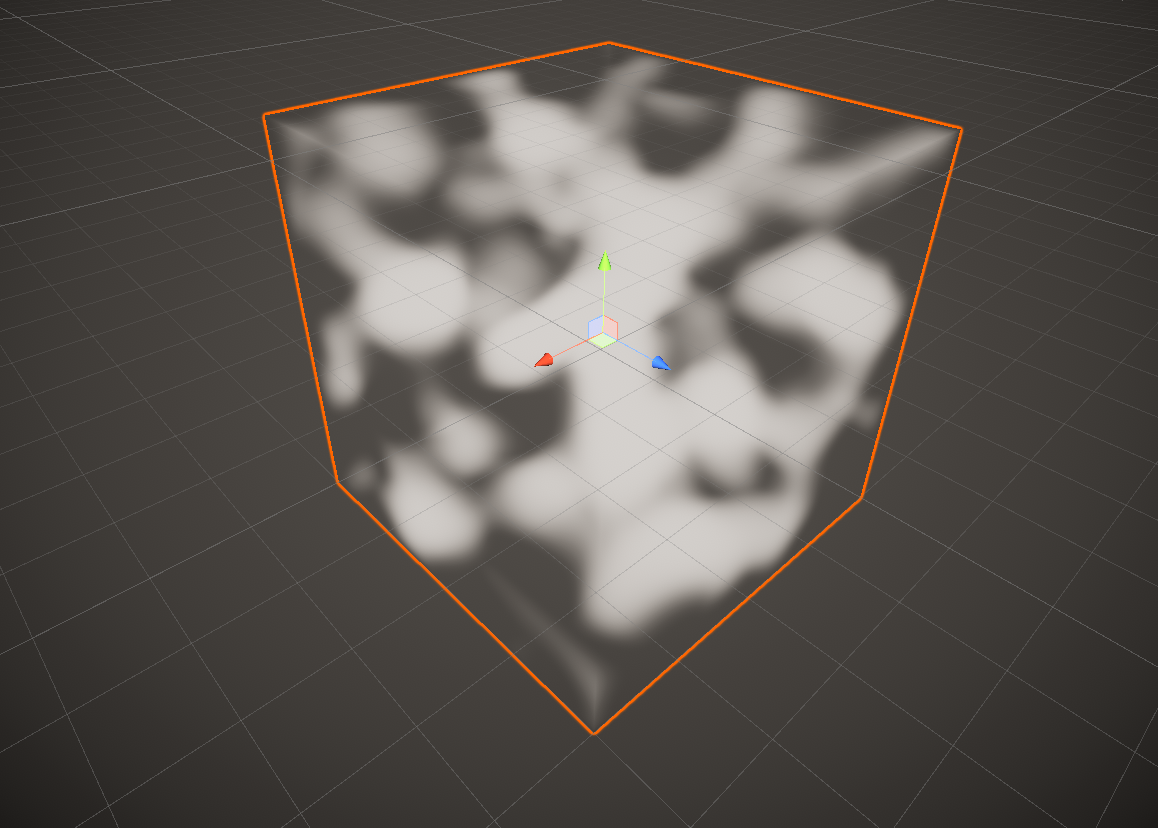
\includegraphics[width=\linewidth]{unity captures/prototype1.PNG}
    \captionof{figure}{Prototype: Rendered image of sampled density based on 3D Perlin noise.}
    \label{img:captures:prototype1}
\end{figure}

\noindent
With this first try, a Perlin noise function was sampled. The returned value had to be normalized in a range of $[0, 1]$ in order for it to be used as alpha value of the color.

\subsubsection{Normalizing Density}
This is where the exponential function $exp(x) = e^{-x}$ comes in, which (when clamped between 0 to 1) converts very low values to 1.0 and higher values will converge towards 0.0.

\begin{figure}[H]
    \centering
    \begin{minipage}{0.47\linewidth}
        \begin{tikzpicture}
            \begin{axis}[
                axis lines=center,
                samples=50,
                xmin=-0.5,
                xmax=4.5,
                ymin=-0.2,
                ymax=1.2,
                xlabel={$x$},
                ylabel={$y$},
                xlabel style={below right},
                ylabel style={above left},
                height=4cm,
                width=8cm,
                ytick={0,1},
                xtick={0,1,2,3,4},
                ]
    
                \addplot[red] plot (\x, { exp(-\x)) });
            \end{axis}
        \end{tikzpicture}
        \captionof{figure}{Exponential function $exp(x) = e^{-x}$.}
        \label{img:math:exp}
    \end{minipage}        
    \hfill
    \begin{minipage}{0.47\linewidth}
        \begin{tikzpicture}
            \begin{axis}[
                axis lines=center,
                samples=50,
                xmin=-0.5,
                xmax=4.5,
                ymin=-0.2,
                ymax=1.2,
                xlabel={$x$},
                ylabel={$y$},
                xlabel style={below right},
                ylabel style={above left},
                height=4cm,
                width=8cm,
                ytick={0,1},
                xtick={0,1,2,3,4},
                ]
    
                \addplot[red] plot (\x, { 1 - exp(-\x)) });
            \end{axis}
        \end{tikzpicture}
        \captionof{figure}{Inverted exponential function $exp'(x) = 1 - e^{-x}$.}
        \label{img:math:exp1}       
    \end{minipage}
\end{figure}

\noindent
When inverting $exp(x)$, the function $exp'(x)$ returns a value that can be directly used for the transparency of the cloud. The denser it gets, the more opaque it will be.

\clearpage
\subsection{Improving Noise}
After further experimenting with the noise sampling function, the idea arose to combine Perlin and Voronoi noise, which hopefully would create a more distinguished, random pattern.
The final sampling function simply multiplies both noise values at a given point \lstinline[language=HLSL]{position}, masking them with each other. 

\begin{lstlisting}[language=HLSL, numbers=left, caption=Implementation of a density sampling function., label=lst:shader:prototype:sampledensity]
float sampleDensity(float3 position) {
  float3 vpos = position * _VoronoiScale + _VoronoiOffset;
  float3 ppos = position * _PerlinScale + _PerlinOffset;
  float vd = fbmVoronoi(vpos, _VoronoiOctaves, _VoronoiPersistence));
  float pd = fbmPerlin(ppos, _PerlinOctaves, _PerlinPersistence));
  
  vd = max(0, vd - _VoronoiDensityThreshold) * _VoronoiDensityMultiplier;
  pd = max(0, pd - _PerlinDensityThreshold) * _PerlinDensityMultiplier;
  
  // fixed boost for density by factor 2
  float density = vd * pd * 2.0;
  return density;
}
\end{lstlisting}

\noindent
By adjusting some of the \gls{parameters} and increasing the octaves of both noises, a more patchy and cloudy look can be achieved at the cost of performance.

\begin{figure}[H]
    \centering
    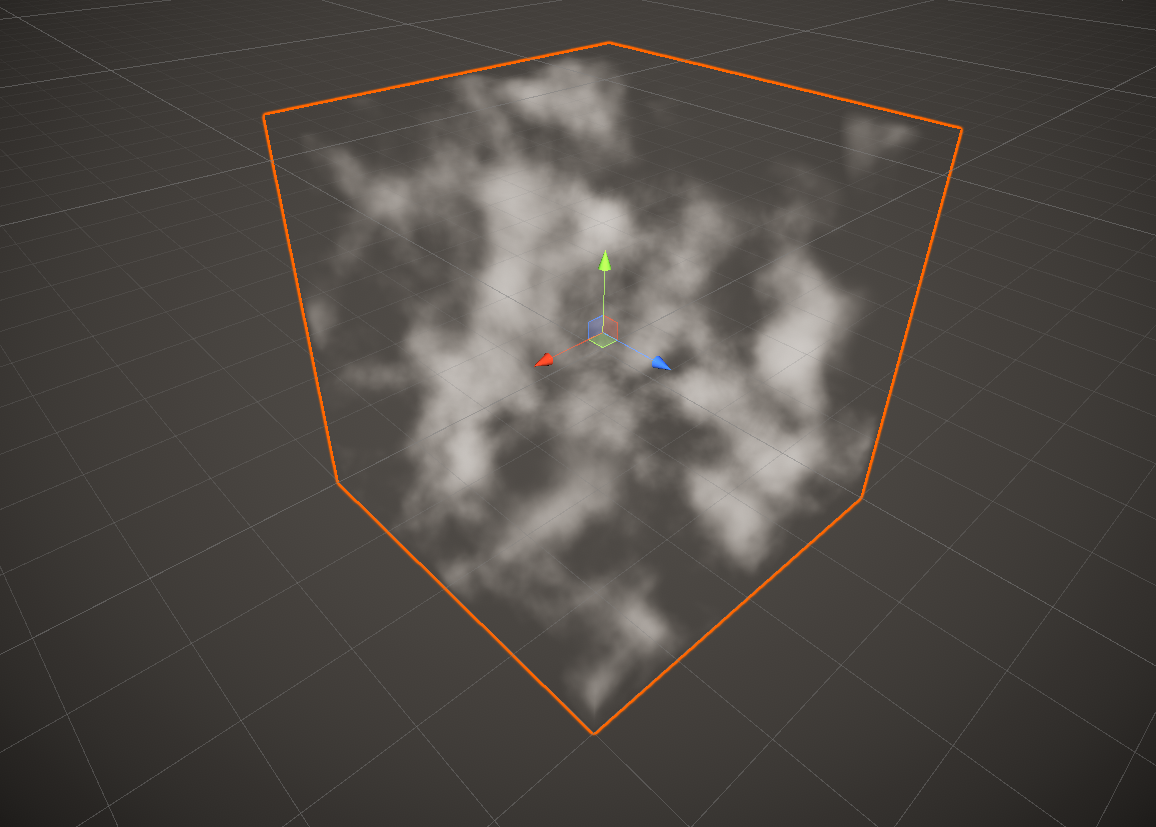
\includegraphics[width=\linewidth]{unity captures/prototype2.PNG}
    \captionof{figure}{Prototype: Rendered image of sampled density based on mixed noises.}
    \label{img:captures:prototype2}
\end{figure}

\clearpage
\subsection{Light Transmittance and Light Scattering}
One of the more prominent lighting features of clouds is its translucency. This phenomenon displays how light bounces and scatters inside the matter, then exits at a different point. This is also called \textit{\gls{sss}} (SSS).
It results in illuminated areas where the clouds are thinner, giving it that milky look and "glow" on the outer edge. In nature, \gls{sss} is a very complex and computationally demanding process. For computer graphics however, it is often either simplified or substituted with some other algorithm that produces a similar outcome at lower performance cost.

\subsubsection{Sunlight Forward Scattering}
When approaching the implementation of \gls{sss} and directional lighting, it seemed most reasonable to start with the sun being visible behind the clouds, or at least shining through them.
This implies finding a way to illuminate clouds that cover the sun. In the context of this project, it is called \textit{\gls{sunlighttransmittance}} or \textit{\gls{sunlightforwarding}}, since it is not a variant of SSS but rather an approximation.
\\
After some consideration and brainstorming, the following method was chosen to solve the issue:

\begin{figure}[H]
    \centering
    \begin{tikzpicture}[scale=1.2]
        \tikzset{edge/.style = {-{Latex[length=3mm]},shorten >= -4pt}}
        \tikzset{shortedge/.style = {-{Latex[length=3mm]},shorten <=-4pt,shorten >= -4pt}}
        \tikzset{line/.style = {shorten >=-4pt}}
        \tikzset{icon/.style = {font=\Large}}

        % icons
        \node[icon,rotate=35,anchor=west] (cam) at (0, 0) {\faVideoCamera};
        \node[icon] (light) at (8, 6) {\faLightbulbO};
        \node at (8, 6.5) {light source};

        % clouds
        \node (cloud) at (4.0, 5.2) {};
        \node[cloud, rotate=-15, cloud puffs=15.7, cloud, minimum width=3.5cm, minimum height=2.2cm, align=center, draw] (cloud) at (cloud) {};

        % screen space
        \draw (1,1) -- (5,0) -- (5,3);

        % rays
        \node[red] (p1) at (3, 2.25) {\ding{53}};
        \node[red] (st1) at ($(p1) + (0.5, -0.2)$) {$st_2$};

        \node[cyan,mark=x] (c1) at (2.4, 2.4) {\ding{53}};
        \node[cyan] (st2) at ($(c1) + (-0.5, 0.2)$) {$st_1$};

        \node (p2) at (5, 3.75) {};
        \node (c2) at (4, 4) {};
        \node[cyan] (c3) at (4.9, 4.9) {\textbullet};

        \draw[red, line] (cam) -- (p1);
        \draw[red, line, loosely dashed] (p1) -- (p2);
        \draw[red, edge, loosely dashed] (p2) -- (light);
        
        \draw[cyan, line] (cam) -- (c1);
        \draw[cyan, line, loosely dashed] (c1) -- (c2);
        \draw[cyan, edge, loosely dashed] (c2) -- (c3);

        % rest of screen space
        \draw (5,3) -- (1,4) node[midway,above,sloped,xshift=-1cm] {screen space} -- (1,1);

        \end{tikzpicture}
    \captionof{figure}{Sunlight transmittance sampling.}
    \label{img:tikz:prototypes:sunlight}
\end{figure}

\noindent
When ray casting, both the fragment's and the light source's screen-space position is calculated. Those are two-dimensional coordinates relative to the screen that the camera renders to.
Now if the distance $d = \norm{\overrightarrow{st_1 st_2}} < t$, with $t$ being some threshold, a portion of the sun's color is added to the fragment's color, relative to how small $d$ is.
\\
It is noteworthy that when calculating the screen-space position, the depth value gets lost. Therefore, theoretically, the clouds would be illuminated when $d < t$ even if the sun is in front of the clouds.
Given this is almost never the case in games and weather simulations, that particular issue is neglected.
\\
Also, instead of evaluating the distance $d$, the intermediate angle of both vectors could also be used to avoid calculating the screen-space position, giving $d = cos^{-1}\left(\overrightarrow{v_{cloud}} * \overrightarrow{v_{light}}\right)$.

\begin{figure}[H]
    \centering
    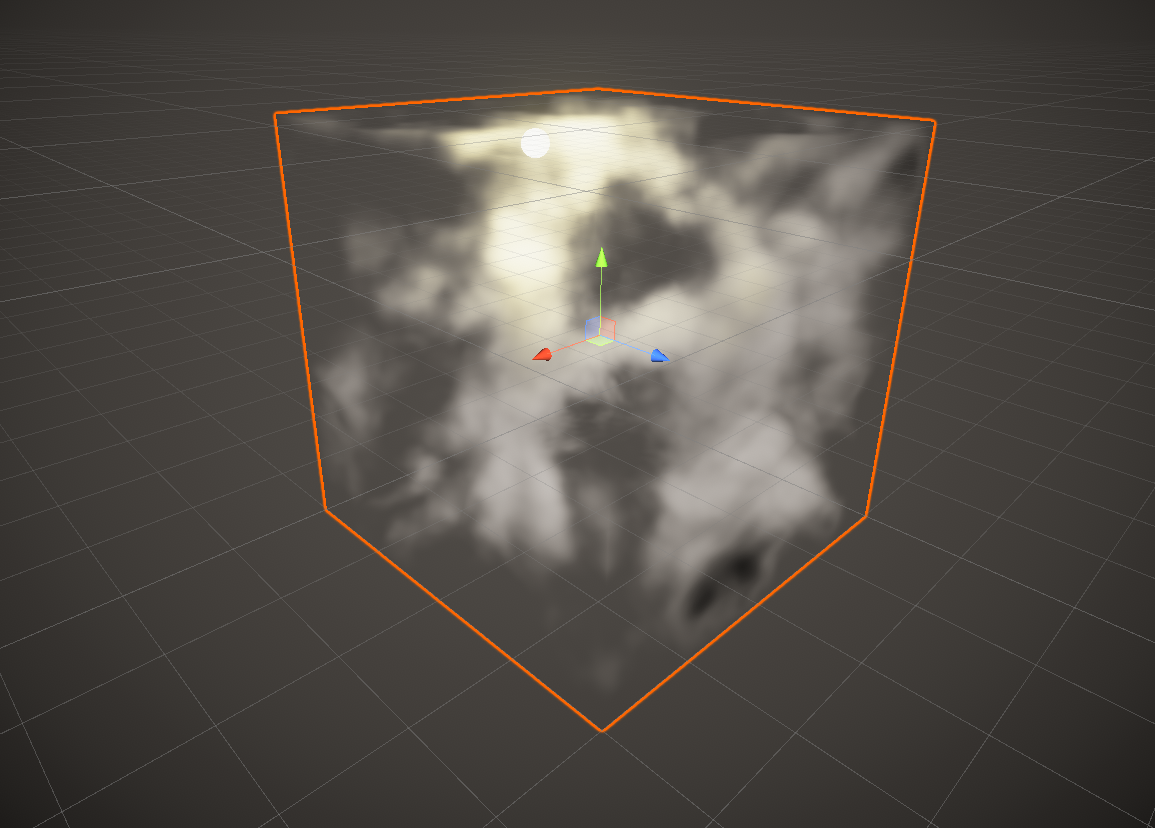
\includegraphics[width=\linewidth]{unity captures/prototype4.PNG}
    \captionof{figure}{Prototype: Rendered image of sunlight transmittance.}
    \label{img:captures:prototype3}
\end{figure}

\noindent
Behind the cube in \autoref{img:captures:prototype3} is a sphere object placed, representing the sun. The sunlight is indeed shining through the clouds, but there are still some minor flaws with the implementation.
For example, some clouds are completely illuminated, making them too bright where the cloud would be too dense for the light to pass through.
\emptyline
The following code snippet shows the implementation of the sunlight transmittance mechanism. The \lstinline[language=HLSL]{density} variable is the one evaluated in \autoref{lst:shader:prototype:sampledensity}.

\begin{lstlisting}[language=HLSL, caption=Implementation of a sunlight transmittance mechanism., label=lst:shader:prototype:sunlighttransmittance]
float cloudDensity = exp(-density);

float projectedSunDistance = length(
  worldToScreenPos(_SunPosition) - worldToScreenPos(worldPosition));

float sunTransmittance = 1 - pow(
  smoothstep(0.01, _SunLightScattering,projectedSunDist), _SunLightStrength);

fixed3 sunColor = sunTransmittance * _LightColor0.xyz * cloudDensity;
\end{lstlisting}

\noindent
Like in other prototype code listings, there are some \gls{parameters} to play with. The sunlight strength or the sunlight range (in screen space) can both be adjusted, for example.
\\
The idea of multiplying by \lstinline[language=HLSL]{cloudDensity} on line 9 was to fix the previously described flaw of clouds being too bright. 

\clearpage
\subsubsection{Directional light}
Another challenging part during prototyping was directional light on surfaces facing the sun. Usually in \gls{raymarching}, a \gls{surfacenormal} estimation is done using the gradient.
This works well if there is only one point of interest (like a ray-surface intersection point), but as already mentioned before, the ray does not stop sampling points until it reaches the end of the container cube.
\\
So instead of calculating normals for each sample point, another ray is cast from the sample point towards the sun.
Along its path, the density is sampled again $L$ times in constant steps. With the lack of an official term, this process is called \textit{\gls{lightmarching}} in this project.

\begin{figure}[H]
    \centering
    \begin{tikzpicture}[scale=1]
        \tikzset{edge/.style = {-{Latex[length=3mm]},shorten >= -4pt}}
        \tikzset{shortedge/.style = {-{Latex[length=3mm]},shorten <=-4pt,shorten >= -4pt}}
        \tikzset{lightedge1/.style = {-{Latex[length=3mm]},shorten <=-4pt,shorten >= 0.8cm}}
        \tikzset{lightedge2/.style = {-{Latex[length=3mm]},shorten <=-4pt,shorten >= 0.85cm}}
        \tikzset{lightedge3/.style = {-{Latex[length=3mm]},shorten <=-4pt,shorten >= 0.90cm}}
        \tikzset{icon/.style = {font=\Large}}

        % icons
        \node[icon,rotate=35,anchor=west] (cam) at (1, 0.75) {\faVideoCamera};
        \node[icon] (light) at (1, 6) {\faLightbulbO};
        \node at (1, 6.5) {light source};

        % clouds
        \node (cloud) at (4.5, 3.5) {};
        \node[cloud, cloud puffs=15.7, cloud ignores aspect, minimum width=5cm, minimum height=3.5cm, align=center, draw] (cloud) at (cloud) {};

        % outer point
        \node (pOut) at (7, 5.25) {};

        % rays
        \draw[red, edge] (cam) -- (pOut) node[midway,above,sloped,xshift=-3cm] {};
        
        % cloud points
        \node[red] (p1) at (3.5, 2.625) {\textbullet};
        \node[red] (p2) at (4.5, 3.375) {\textbullet};
        \node[red] (p3) at (5.5, 4.125) {\textbullet};
        \node[red] (p4) at (4.5, 3.375) {\textbullet};
        \node[red] (p5) at (5.5, 4.125) {\textbullet};

        % light march rays
        \draw[cyan, lightedge1] (p1) -- (light) node[midway,above] {};
        \draw[cyan, lightedge2] (p2) -- (light) node[midway,above] {};
        \draw[cyan, lightedge3] (p3) -- (light) node[midway,above,yshift=0.5cm] {lightmarch rays};

        % light sample points
        \node[cyan] (l1) at (3.25, 2.95) {\textbullet};
        \node[cyan] (l2) at (4.15, 3.625) {\textbullet};
        \node[cyan] (l3) at (5.0, 4.325) {\textbullet};
        
        \node[cyan] (l5) at (3.0, 3.3) {\textbullet};
        \node[cyan] (l6) at (3.75, 3.95) {\textbullet};
        \node[cyan] (l7) at (4.5, 4.55) {\textbullet};
        
        \node[cyan] (l8) at (2.75, 3.65) {\textbullet};
        \node[cyan] (l9) at (3.35, 4.22) {\textbullet};
        \node[cyan] (l10) at (3.95, 4.775) {\textbullet};

        \end{tikzpicture}
    \captionof{figure}{Directional lightmarching samples (part 1).}
    \label{img:tikz:prototypes:lightmarching1}
\end{figure}

\noindent
It is clearly visible that in \autoref{img:tikz:prototypes:lightmarching1}, a lot of density samples return a high value, resulting in a dark fragment color for this ray.
To simplify, there is a lot of cloud mass in front of that sample point, so the fragment will not receive a lot of sunlight color.
\\
On the other hand, in \autoref{img:tikz:prototypes:lightmarching2}, only very few samples are even inside the cloud, resulting in a low value overall. This leads to a higher influence of the sun's color for that fragment, meaning the samples are more exposed to the sun.

\begin{figure}[H]
    \centering
    \begin{tikzpicture}[scale=1]
        \tikzset{edge/.style = {-{Latex[length=3mm]},shorten >= -4pt}}
        \tikzset{shortedge/.style = {-{Latex[length=3mm]},shorten <=-4pt,shorten >= -4pt}}
        \tikzset{lightedge1/.style = {-{Latex[length=3mm]},shorten <=-4pt,shorten >= 0.8cm}}
        \tikzset{lightedge2/.style = {-{Latex[length=3mm]},shorten <=-4pt,shorten >= 0.85cm}}
        \tikzset{lightedge3/.style = {-{Latex[length=3mm]},shorten <=-4pt,shorten >= 0.90cm}}
        \tikzset{icon/.style = {font=\Large}}

        % icons
        \node[icon,rotate=35,anchor=west] (cam) at (1, 0.75) {\faVideoCamera};
        \node[icon] (light) at (1, 6) {\faLightbulbO};
        \node at (1, 6.5) {light source};

        % clouds
        \node (cloud) at (5.7, 2.7) {};
        \node[cloud, cloud puffs=15.7, cloud ignores aspect, minimum width=5cm, minimum height=3.5cm, align=center, draw] (cloud) at (cloud) {};

        % outer point
        \node (pOut) at (7, 5.25) {};

        % rays
        \draw[red, edge] (cam) -- (pOut) node[midway,above,sloped,xshift=-3cm] {};
        
        % cloud points
        \node[red] (p1) at (3.5, 2.625) {\textbullet};
        \node[red] (p2) at (4.5, 3.375) {\textbullet};
        \node[red] (p3) at (5.5, 4.125) {\textbullet};
        \node[red] (p4) at (4.5, 3.375) {\textbullet};
        \node[red] (p5) at (5.5, 4.125) {\textbullet};

        % light march rays
        \draw[cyan, lightedge1] (p1) -- (light) node[midway,above] {};
        \draw[cyan, lightedge2] (p2) -- (light) node[midway,above] {};
        \draw[cyan, lightedge3] (p3) -- (light) node[midway,above,yshift=0.5cm] {lightmarch rays};

        % light sample points
        \node (l1) at (3.25, 2.95) {\textopenbullet};
        \node[cyan] (l2) at (4.15, 3.625) {\textbullet};
        \node (l3) at (5.0, 4.325) {\textopenbullet};
        
        \node (l5) at (3.0, 3.3) {\textopenbullet};
        \node (l6) at (3.75, 3.95) {\textopenbullet};
        \node (l7) at (4.5, 4.55) {\textopenbullet};
        
        \node (l8) at (2.75, 3.65) {\textopenbullet};
        \node (l9) at (3.35, 4.22) {\textopenbullet};
        \node (l10) at (3.95, 4.775) {\textopenbullet};

        \end{tikzpicture}
    \captionof{figure}{Directional lightmarching samples (part 2).}
    \label{img:tikz:prototypes:lightmarching2}
\end{figure}

\clearpage
\noindent
The implementation for \gls{lightmarching} is rather straight-forward, given the concept of \gls{raymarching} is already known.

\begin{lstlisting}[language=HLSL, caption=Implementation of lightmarching., label=lst:shader:prototype:lightmarching]
float lightmarch(float3 position, float3 direction) {
    float3 p = position;

    float lightTransmittance = 0;
    for (int j = 0; j < _MaxLightSteps; j++)
    {
        p += direction * _LightStepSize;
        lightTransmittance += sampleDensity(p);
    }

    return lightTransmittance;
}
\end{lstlisting}

\noindent
The method is called during \gls{raymarching} and the original function is modified like so:
\begin{lstlisting}[language=HLSL,caption=Implementation of raymarching with lightmarching., label=lst:shader:prototype:raylightmarching]
float2 raymarch(float3 position, float3 direction)
{
    float3 sunDirection = normalize(_SunPosition - position);
    float lightStepSize = insideBoxDist / _MaxLightSamples;
    float lightTransmittance = 0;

    [...ray marching...]
    
    for (int j = 0; j < _MaxLightSamples; j++)
    {
        position += direction * lightStepSize;
        lightTransmittance += lightmarch(position, sunDirection);
    }

    return float2(density, lightTransmittance);
}
\end{lstlisting}

\noindent
Now, two values are returned instead of just one. Both are later normalized with either $exp(x)$ or $exp'(x)$.

\begin{figure}[H]
    \centering
    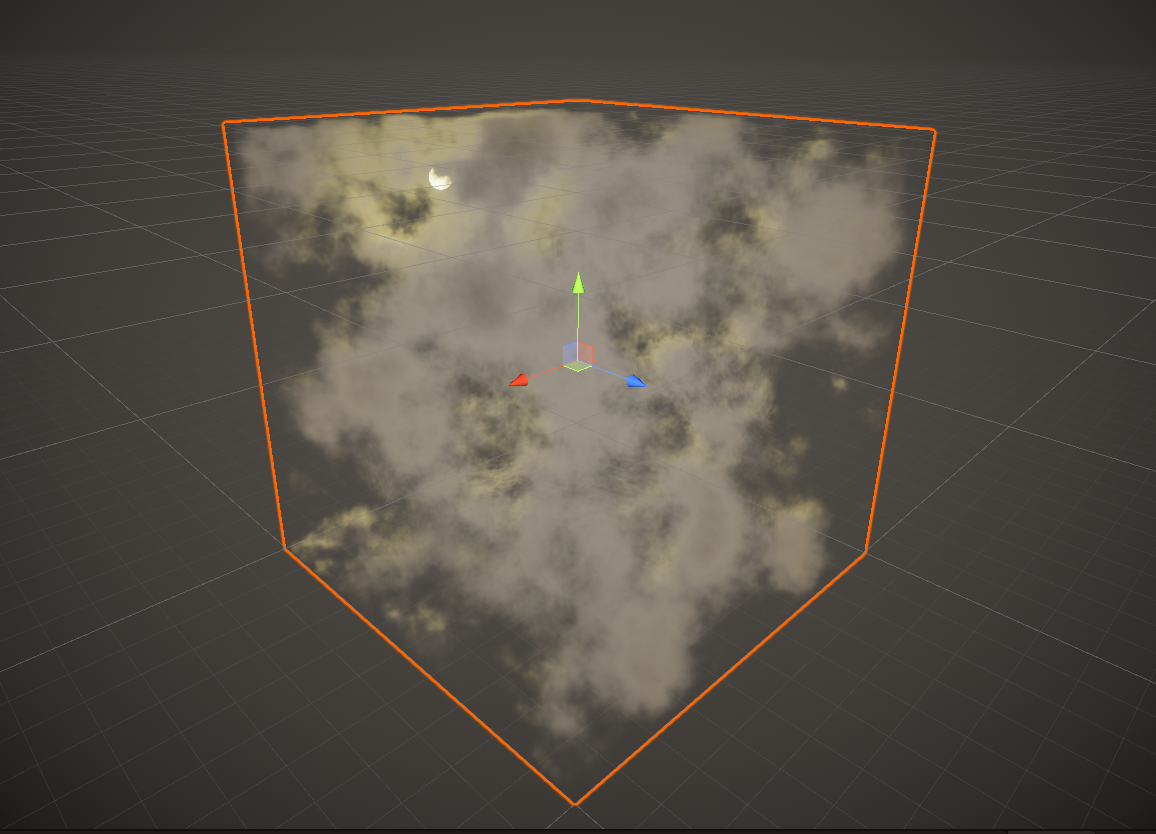
\includegraphics[width=\linewidth]{unity captures/prototype5.PNG}
    \captionof{figure}{Prototype: Rendered image of directional sunlight implemented with \gls{lightmarching}.}
    \label{img:captures:prototype5}
\end{figure}

\clearpage
\subsection{Final Prototype}
All put together and after quite some effort and experimenting, the rendered scene looks quite convincing. 
\\
Free assets from the Unity Asset Store were used for trees\footnote[1]{https://assetstore.unity.com/packages/3d/vegetation/speedtree/free-speedtrees-package-29170} and rocks\footnote[2]{https://assetstore.unity.com/packages/3d/environments/landscapes/photoscanned-moutainsrocks-pbr-130876}.

\begin{figure}[H]
    \centering
    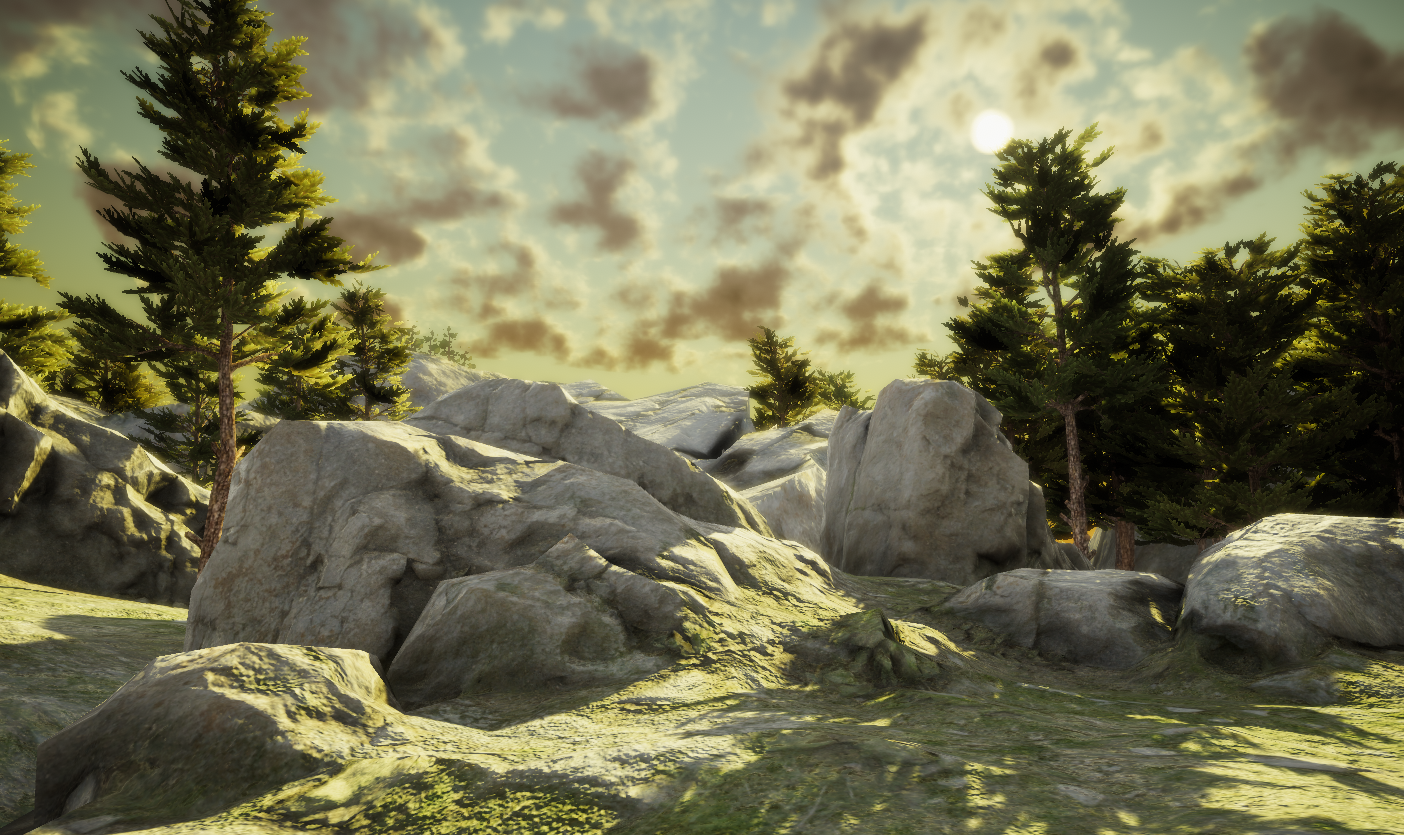
\includegraphics[width=\linewidth]{unity captures/final_dusk.PNG}
    \captionof{figure}{Prototype: Rendered image of the final prototype (afternoon scene).}
    \label{img:captures:prototype_final:afternoon}
\end{figure}

\clearpage
\noindent
To demonstrate the capability of the shader in its prototype state, here are some variations of it. The are no code changes in-between the rendered images, the only things that changed are the shader's \gls{parameters} and Unity Editor lighting settings and colors.

\begin{figure}[H]
    \centering
        \begin{minipage}{0.47\linewidth}
            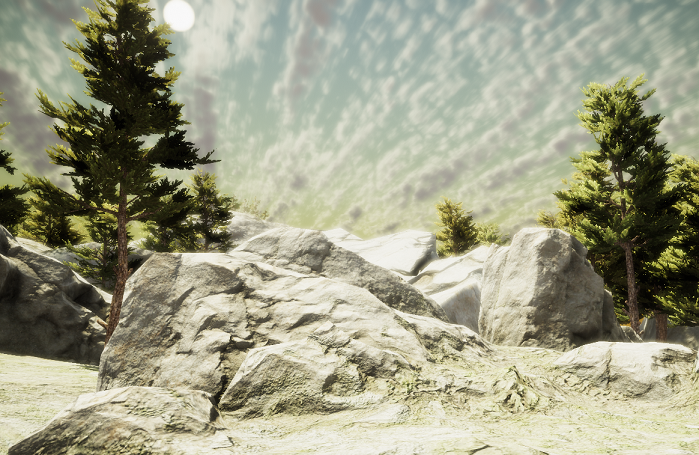
\includegraphics[width=\linewidth]{unity captures/final doc/final_day_small.PNG}
            \captionof{figure}{Prototype: Rendered day scene.}
            \label{img:captures:prototype_final:day}
        \end{minipage}
    \hfill
        \begin{minipage}{0.47\linewidth}
            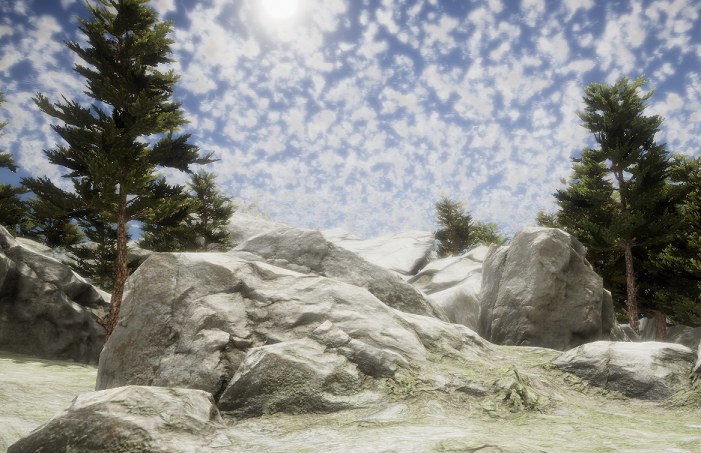
\includegraphics[width=\linewidth]{unity captures/final doc/final_puffy_small.PNG}
            \captionof{figure}{Prototype: Rendered puffy sky scene.}
            \label{img:captures:prototype_final:puffy}
        \end{minipage}
\end{figure}

\begin{figure}[H]
    \centering
        \begin{minipage}{0.47\linewidth}
            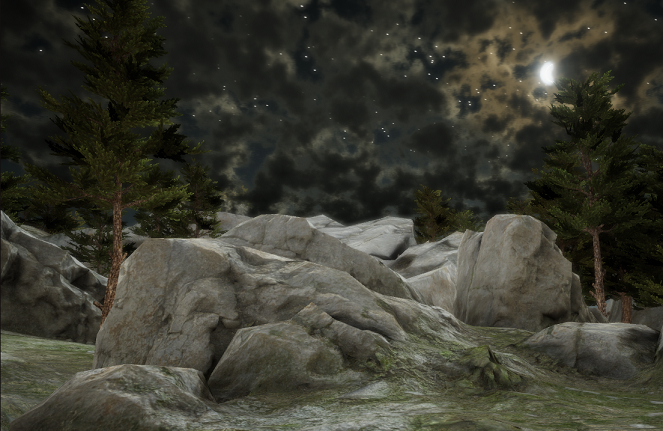
\includegraphics[width=\linewidth]{unity captures/final doc/final_night_small.PNG}
            \captionof{figure}{Prototype: Rendered night scene.}
            \label{img:captures:prototype_final:night}
        \end{minipage}
    \hfill
        \begin{minipage}{0.47\linewidth}
            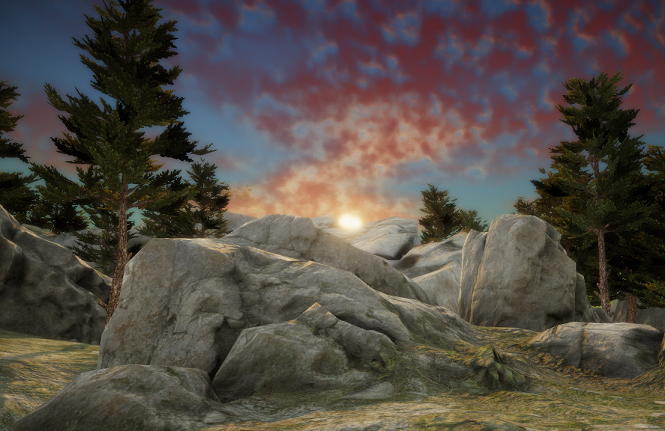
\includegraphics[width=\linewidth]{unity captures/final doc/final_sunset_small.PNG}
            \captionof{figure}{Prototype: Rendered sunset scene.}
            \label{img:captures:prototype_final:sunset}
        \end{minipage}
\end{figure}

\begin{figure}[H]
    \centering
        \begin{minipage}{0.47\linewidth}
            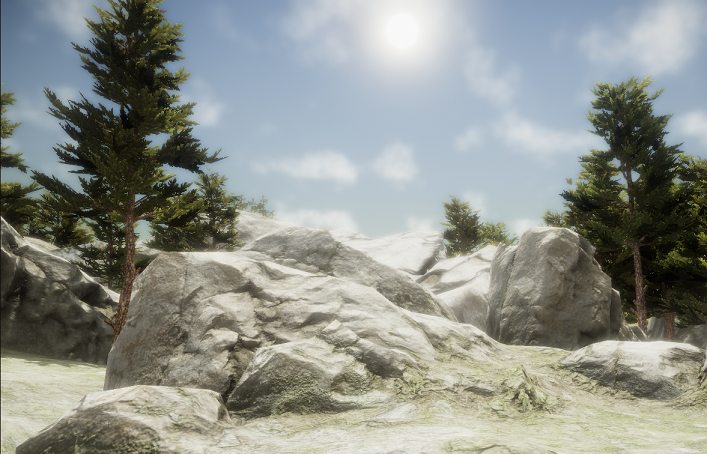
\includegraphics[width=\linewidth]{unity captures/final doc/final_clear_small.PNG}
            \captionof{figure}{Prototype: Rendered clear sky scene.}
            \label{img:captures:prototype_final:clear}
        \end{minipage}
    \hfill
        \begin{minipage}{0.47\linewidth}
            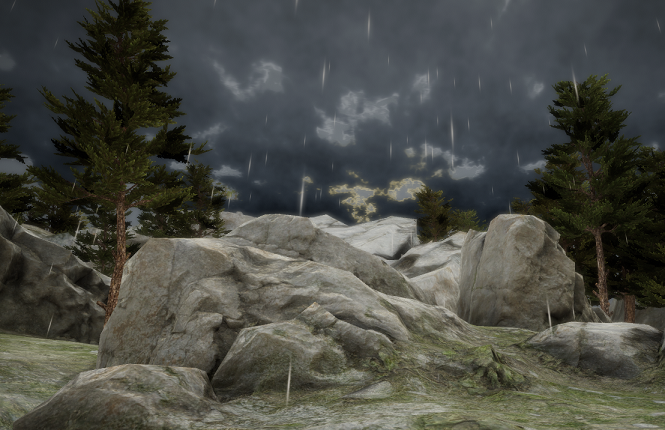
\includegraphics[width=\linewidth]{unity captures/final doc/final_stormy_small.PNG}
            \captionof{figure}{Prototype: Rendered stormy scene.}
            \label{img:captures:prototype_final:stormy}
        \end{minipage}
\end{figure}

\clearpage
\subsubsection{Additional Masking}
Technically, by multiplying both noise function values in \lstinline[language=HLSL]{sampleDensity()}, they already mask each other. In certain types of cloud formations, an additional masking needs to be applied in order to create a cloudscape that does not expand over the whole container cube.
This is done by feeding a mask texture into the shader, for which the cube's UV coordinates are used to sample the grey value of the texture at that position.

\begin{figure}[H]
    \centering
    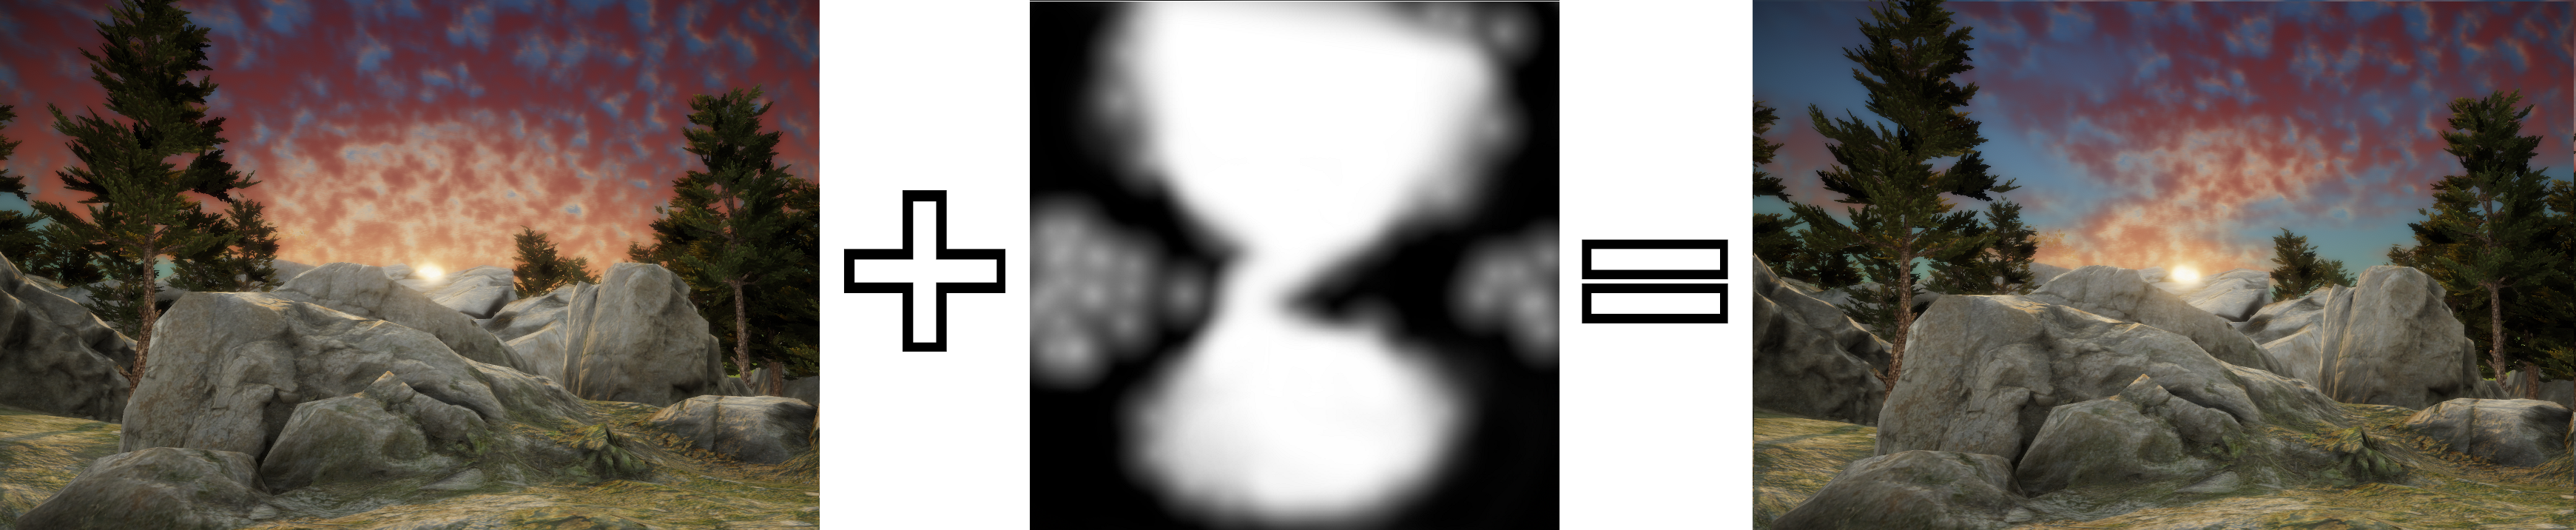
\includegraphics[width=\linewidth]{comparisons/masking.png}
    \captionof{figure}{Prototype: Masking with UV coordinates of the container cube.}
    \label{img:camparisons:masking}
\end{figure}

\clearpage
\subsection{Realism Check}
\label{section:prototypes:realismcheck}
While the prototypes in \autoref{img:captures:prototype_final:day} to \autoref{img:captures:prototype_final:stormy} do look realistically to a certain degree, it is still essential to have some sort of measurable factor with which the rendered images can be compared to real clouds.
Some factor that ultimately shows how \textit{real} the rendered clouds actually are, apart from the human eye interpretation.

\subsubsection{Objective interpretation}
Before expanding on how to measure the realism of the cloud shader's output, it seems important to objectively identify the capabilities of it first.
As originally stated in \sectionref{section:clouds-in-games}, the desired look of the clouds was that of the genus \textit{cumulus}.
\\
In the following subsection, each rendered image is compared to a real-life photograph, putting them into a objectively comparable state to reality.

\clearpage
\subsubsection{Real Life Comparison}
In all the following comparison images, the left images are photographic references and the right side images are rendered in Unity Engine.
\emptyline
\autoref{img:captures:prototype_final:day} and \autoref{img:captures:prototype_final:puffy} both resemble cirrocumulus and altocumulus clouds.
The cirrocumulus clouds are similar to altocumulus clouds, but they form at higher altitude and are significantly smaller, yet equally puffy.
\\
\autoref{img:captures:prototype_final:night} and \autoref{img:captures:prototype_final:sunset} also show the distinctive cotton-like pattern of the altocumulus genus.
When comparing to an actual photograph, there are only few differences.
\emptyline
By adjusting the scale of the shader, the clouds can be made smaller. In the following comparison, the directional \gls{lightmarching} has been turned down to a minimum so the light would look more wan. 

\begin{figure}[H]
    \centering
    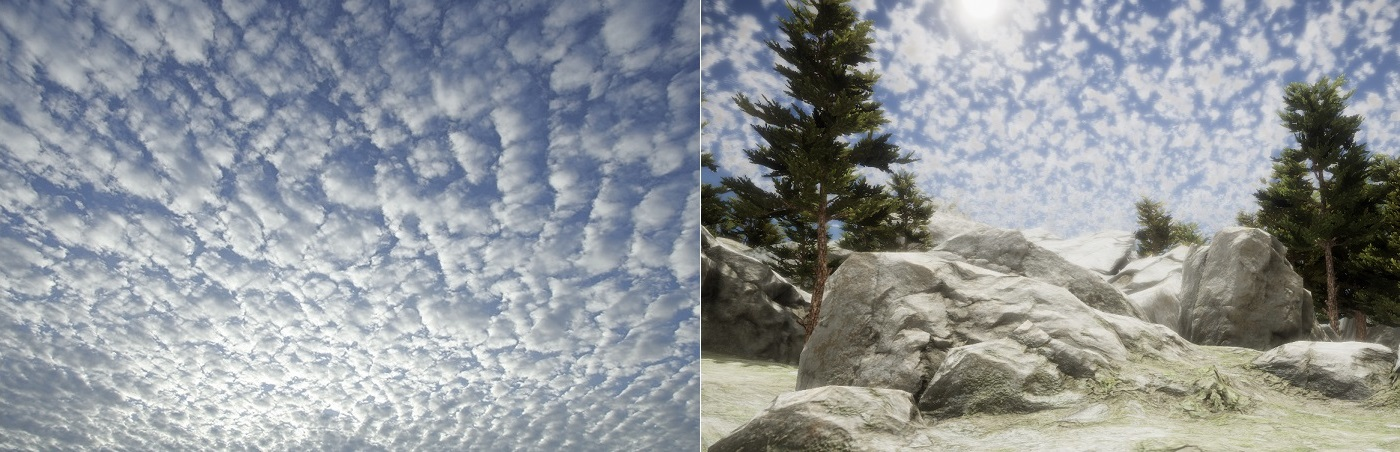
\includegraphics[width=\linewidth]{comparisons/compare_altocumulus.jpg}
    \captionof{figure}{Comparison: photographic reference \protect\cite{img:campare:altocumulus} versus the rendered image.}
    \label{img:comparisons:altocumulus}
\end{figure}

\noindent
The night-time comparison displays how the different color of the \gls{sunlightforwarding} can impact the scene.

\begin{figure}[H]
    \centering
    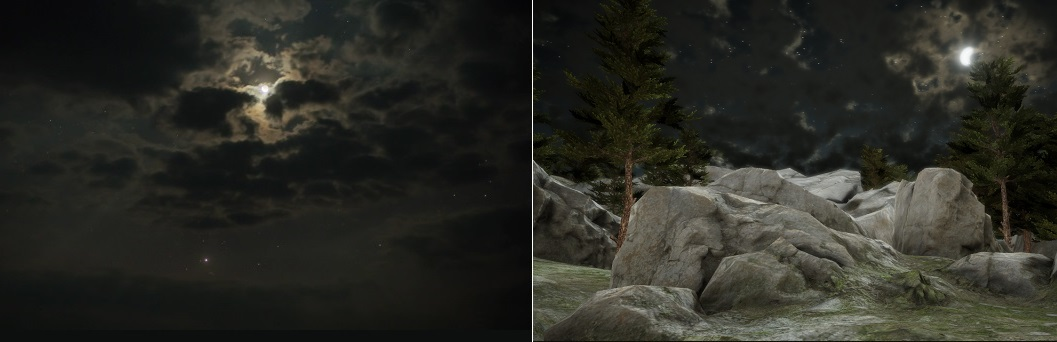
\includegraphics[width=\linewidth]{comparisons/compare_altocumulus_night.jpg}
    \captionof{figure}{Comparison: photographic reference \protect\cite{img:campare:altocumulus:night} versus the rendered image (at night).}
    \label{img:comparisons:altocumulus:night}
\end{figure}

\clearpage
\noindent
In \autoref{img:captures:prototype_final:sunset}, it is very clearly recognizable that the \gls{parameters} of the shader can heavily influence the lighting and illumination of the clouds.
Unfortunately, the difference of details and density is fairly discernable from reality and the desired appearance is not fully achieved.

\begin{figure}[H]
    \centering
    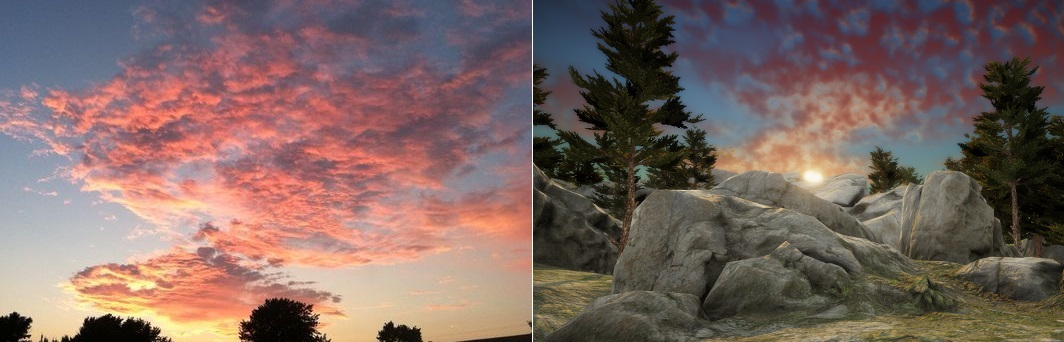
\includegraphics[width=\linewidth]{comparisons/compare_altocumulus_sunset.jpg}
    \captionof{figure}{Comparison: photographic reference \protect\cite{img:campare:altocumulus:sunset} versus the rendered image (at sunset).}
    \label{img:camparisons:altocumulus:sunset}
\end{figure}

\noindent
Finally, \autoref{img:captures:prototype_final:stormy} represents clouds of the type \textit{nimbostratus}, which form in low altitude and are dense and dark, often rainy.


\begin{figure}[H]
    \centering
    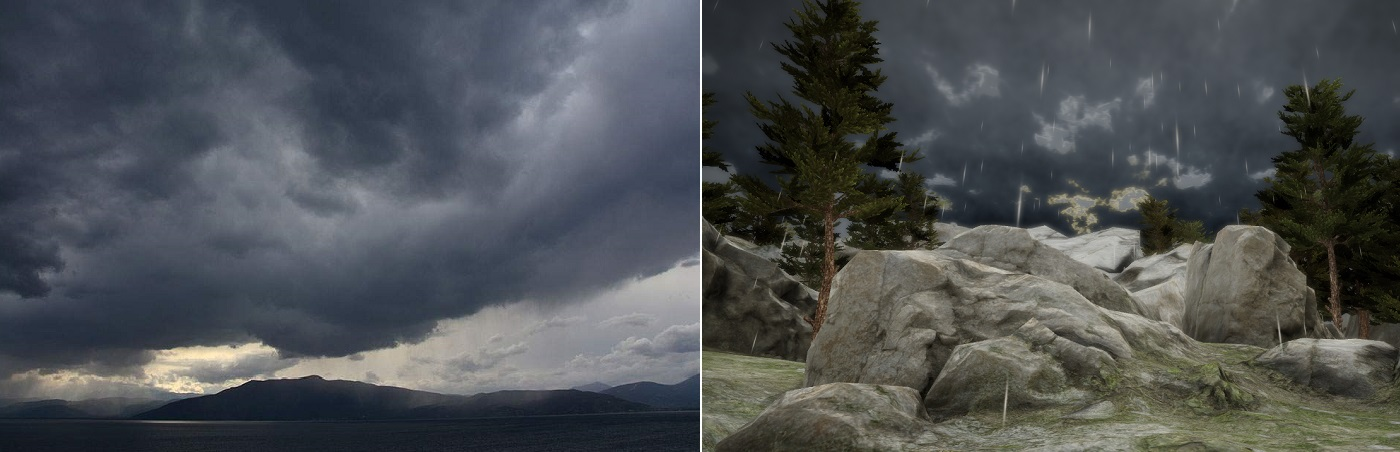
\includegraphics[width=\linewidth]{comparisons/compare_altocumulus_stormy.jpg}
    \captionof{figure}{Comparison: photographic reference \protect\cite{img:campare:altocumulus:stormy} versus the rendered image (stormy).}
    \label{img:camparisons:altocumulus:stormy}
\end{figure}

\noindent
With the \gls{sunlighttransmittance} being a bright yellow in the rendered image, an attempt was made to make the sun shine through the distant rainy clouds, like in the photographic reference. Since the cloud shader does not end before the horizon, the resulting effect is rather imperceptible.

\clearpage
\subsubsection{Convolutional Neural Network}
Given there is a \gls{cnn} (CNN) that is able to classify images of the sky, the weather or clouds into descriptive labels or even genera of cloud formations, then one could just seed those rendered images into the CNN and verify whether the results are truthfully showing "real" clouds.
Of course, this is heavily dependent of how well the CNN was trained.

\subsubsection{Generative Adversarial Network}
A similar approach to the \gls{cnn} is a  \gls{gan} (GAN) setup. It describes two neural networks, which contest with each other in a cat-and-mouse game: The \textit{generative} network tries to imitate the training set by generating artificial photographs with many realistic characteristics, while the \textit{discriminative} network tries to tell whether the generated images are fake or not.
\\
With this method, the rendered cloud images could be passed through the discriminative neural network to see if at least the network thinks the images are of real clouds.

\subsubsection{Histogram Comparison}
The \textit{\gls{histogram}} is a graphical representation of data like brightness or color distribution of a given photograph.
When extracting the color \gls{histogram}s of the real photograph and the one of the rendered image, they could be compared and rated how different in color they are.

\subsubsection{Professional Meteorological Assessment}
Another viable solution is to let a professional meteorologist inspect and rate the rendered images and judge the realism of the depicted scenarios, which should reveal if the rendered clouds could actually form and exist in reality.

\clearpage
\subsection{Performance}
With the current implementations of \gls{raymarching} and \gls{lightmarching}, the performance of the shader is heavily dependent on the number of samples $N$ and $L$ taken along the rays.
With a container cube the size of 400x200 pixel in screen-space (which is a relatively small box of clouds), the \gls{gpu} load is already enormously large. 
Here, the number of noise samplings $N_{total}$ is calculated as follows. The values for $N$ and $L$ are both set to a minimum of 25, since it seemed to achieve the best looking results during prototyping.
$$ 
\begin{array}{l}
    w = 400, h = 200\\
    N = 25, L = 25\\ \\
    N_{total} = w * h * N * L = 5 * 10^7
\end{array}
$$

\noindent
So for a single frame, the number of times the noise function is called for this example is just about fifty million times. This inconceivably high number makes the current implementation desperately needy of optimization.

\subsubsection{Optimization Attempts}
\paragraph{Compute Shader}
The fact that the noise function needs to be sampled so often may not even be the issue, but rather that the noise texture needs to be calculated again each time.
Therefore, the idea arose to precalculate the 3D noise volume and feed it to the shader at runtime, in the form of a 3D texture cube.
\\
For this, a \gls{computeshader} was created with the attempt to generate said texture.
Unfortunately, all experiments with \gls{computeshader}s were unsuccessful, as there is only very little documentation about 3D texture-generating \gls{computeshader}s for Unity Editor.
This attempt was therefore abandoned.

\paragraph{Early Exits}
For some functions and loops, early exit conditions can speed up the shader. As an example in \autoref{lst:shader:prototype:raylightmarching}, which describes \gls{raymarching} combined with \gls{lightmarching}, the light does not need to be calculated when there is no cloud.
The following little extension should fix that issue.
\begin{lstlisting}[language=HLSL]
if (density <= 0) {
    return float2(0, 0);
}
\end{lstlisting}

\noindent
Instead of checking if \lstinline[language=HLSL]{density} is smaller or equal to zero, a very small threshold could be used as well.
It is noteworthy that a number larger than zero can create edges on thin clouds, as the abrupt reduction in density may be visible.
\clearpage

\section{Project Management}
\label{section:projectmanagement}

\subsection{Schedule Comparison}
The following chart shows the original schedule (in grey) with a side-by-side comparison with the actual time spent for each task (in blue). It indicates that the schedule was mostly met throughout the project.
\vspace{\baselineskip}

\begin{ganttchart}[
    vgrid={dotted},
    hgrid={draw=black!50, dotted},
    bar/.append style={fill=lightgray},
    x unit=0.65cm,
    ms/.append style={milestone/.append style={fill=gray, scale = 0.7, yshift=0.2cm}},
    ms2/.append style={milestone/.append style={fill=cyan, scale = 0.7, yshift=-0.2cm}},
    progress label text={},
    bar1/.append style={bar height=0.2},
    bar2/.append style={bar height=0.2},
    bar2/.append style={bar top shift=0.018cm},
    ]{1}{16}
    \gantttitle{Work weeks}{16} \\
    \gantttitlelist{1,...,16}{1} \\
    \ganttbar[bar1]{Organization}{1}{4}
    \ganttbar[bar2, bar/.append style={fill=cyan}]{}{1}{4} \\
    \ganttmilestone[ms]{Specification finished}{4}
    \ganttmilestone[ms2]{}{4} \\
    \ganttgroup{Documentation}{5}{15} \\
    \ganttbar[bar1]{Research}{5}{11}
    \ganttbar[bar2, bar/.append style={fill=cyan}]{}{5}{13} \\
    \ganttbar[bar1]{Prototyping}{7}{15}
    \ganttbar[bar2, bar/.append style={fill=cyan}]{}{7}{15} \\
    \ganttmilestone[ms]{Prototype 1 finished}{9}
    \ganttmilestone[ms2]{}{9} \\
    \ganttmilestone[ms]{Prototype 2 finished}{11}
    \ganttmilestone[ms2]{}{15} \\
    \ganttmilestone[ms]{Prototype 3 finished}{15} \\
    \ganttbar[bar1]{Finalizing}{16}{16}
    \ganttbar[bar2, bar/.append style={fill=cyan}]{}{16}{16}
\end{ganttchart}

\vspace{\baselineskip}
\noindent
As explained in \sectionref{section:projectmanagement:goals}, "prototype 3" was removed from the schedule, which is why the blue milestone is missing.
Since there was now more time available for the other prototype, the milestone for "prototype 2" was moved to the end of the segment.

\subsection{Goal Discrepancies}
\label{section:projectmanagement:goals}
Originally, the following three prototypes were planned.
\begin{itemize}
    \item \gls{volumetricrendering}
    \item \gls{procedural} \gls{noise} generation
    \item \gls{raymarching}
\end{itemize}
During research and prototyping, it came clear that "\gls{raymarching}" is in fact a substantial part of \gls{volumetricrendering} instead of a completely different topic.
Hence, only two of the three listed prototypes were implemented. This change led to a significant boost in available development time for the other two prototypes, for which the results could now be finalized to a greater extent.

\subsection{Future Work}
The final prototype is a solid basis for future projects, such as rendering of more cloud genera like the infamous, high-towering cumulonimbus clouds, performance optimizations and much more.

\subsubsection{Complete Weather System}
Another wonderful idea is to expand the shader into a fully-fledged weather system. Instead of having all the those technical \gls{parameters}, it would instead be dependent on temperature, humidity, altitude, highs and lows, weather fronts and many other real meteorological variables.
It would automatically start to rain when the the conditions are met and the cloud shader movement would adjust itself by the wind strength and direction \gls{parameters}.

\subsubsection{Extensive Lighting Features}
Despite the considerable effort already put into lighting and illumination methods, there are still some features missing. One of those are \textit{god rays}, the volumetric light shafts that shine through gaps in clouds, giving the scene even more depth.
Other absent features are the sun's and moon's halo: A bright circle around the celestial body.

\subsubsection{Measure Realism}
As described in \sectionref{section:prototypes:realismcheck}, there are several possible approaches to measure the realism of the clouds. This opens up potential for a future project.

\subsection{Project Conclusion}
It is noteworthy that two more weeks were put into research. This is mainly because new methods and algorithms have been continuously researched during prototyping, which resulted in constant documentation of those findings.
However, this did not conflict with the rest of the schedule.
\\
Still, the total amount of time spent was about ten percent more than the originally estimated time budget of 128 hours. This is probably due to the fact that there was quite some effort put into the final prototype.
\\
The project occurred during the same time as the global coronavirus lockdown phase, but was unhindered by that.
\emptyline
In summary, all project requirements were met, the milestones were completed in time and the final prototype turned out great, making this a successful and very informative project.
\clearpage

\printnoidxglossary 
\clearpage
\printbibliography[heading=bibintoc]
\clearpage
\phantomsection
\addcontentsline{toc}{section}{Listings}
\phantomsection
\addcontentsline{toc}{subsection}{Figures}
\listoffigures
\clearpage
\phantomsection
\addcontentsline{toc}{subsection}{Code Listings}
\lstlistoflistings

\end{document}
